% TODO check figure captions
\chapter{Double-Differential Muon Neutrino Charged Current Inclusive Measurement} \label{sec:NewCCInclusive}
This chapter exists because of my long writing process for this thesis. It contains the most recent \gls{cc} inclusive measurement, which is a forward-folded double differential cross section as a function of $\cos{(\theta)}$, and the momentum $p_\mu$ of the muon. The content of this chapter is derived from T. Mettler's PhD Thesis \cite{CRTThomasPhD} and constitutes a publication in progress by our group for the MicroBooNE collaboration. For practical reasons I will heavily reference my first analysis described in chapter \ref{sec:FistCCInclusive}.

\section{TPC and Monte Carlo Data Samples} \label{sec:AnalysisSamples}
The data used in this analysis was taken in the period between December 2017 and Summer 2018, when \gls{crt} data was available in good quality. Before this period, the \gls{crt} was either incomplete or event timing was treated differently. As in the analysis presented before in chapter \ref{sec:FistCCInclusive}, we use two kinds of \gls{tpc} data samples: one with \textbf{beam on} and another \textbf{beam off}. For the beam on selection a ``run 3'' data set of \num{2.1e20} \gls{pot} was unblinded in accordance with MicroBooNE's data blindness policy. The trigger logic for this beam on sample requires a \gls{Flash} in the \SI{1.6}{\micro\second} \gls{bnb} window. The beam on sample is expected to consist of mostly cosmic background events, caused by a random cosmic-ray \gls{Flash} coincidence with a \gls{BeamGate}. As before, this background is easily measured resulting in the beam off sample. Said sample was triggered by an external random \gls{BeamGate} signal and a cosmic-ray induced \gls{Flash} in the same \SI{1.6}{\micro\second} time window. This ``fake'' beam trigger setup is also known as \textbf{BNBEXT}. Note, both \gls{tpc} data sets use the same trigger logic as in the measurement described previously in section \ref{sec:DataSamples}. The \gls{tpc} data samples utilised in this most recent \gls{cc} inclusive analysis are listed in table \ref{tab:NewDataSamples} below. Also listed there, one finds the version number of the \textbf{uboonecode} used for reconstruction. 
\begin{table}[htbp]
    \centering
    \caption[Detector Data Samples Used in the New Analysis]{These are the two recorded data samples (beam on and beam off), used in this \gls{cc} inclusive analysis. $N^\text{Trig}$ stands for the total number of recorded events, \ie number of \gls{Flash} plus \gls{BeamGate} triggers received.}
    \begin{tabu}{llrrr}
        \toprule
        \rowfont[c]{\bf} Sample name & Trigger & $N^\text{Trig}$ & \gls{pot} & uboonecode \\
        \midrule
        beam on & \gls{bnb} & \num{51546294} & \num{2.144e20} & v08.00.00.50 \\
        beam off & \textbf{BNBEXT} & \num{85768579} & \multicolumn{1}{c}{N/A} & v08.00.00.25 \\
        \bottomrule
        \label{tab:NewDataSamples}
    \end{tabu}
\end{table}
The beam off sample then needs to be scaled in order to match the beam on sample's \gls{pot}. This is achieved by scaling the number of beam off triggers, $N_\text{EXT}^\text{Trigg}$, to the number of \glspl{BeamGate} of the beam on sample, as shown before in equation \ref{eq:NumberOfNu}.

There are two \gls{mc} samples used in this analysis: one is the \gls{bnb} \textbf{overlay} sample and the other is called \textbf{Dirt overlay}. The former has neutrino events generated in the \gls{tpc} volume of the detector, while the latter has them generated outside of the \gls{tpc}, hence the designation ``Dirt''. The event generator used to produce the samples was \gls{genie} v3.0.6 G18.10a.02.11a with a preliminary MicroBooNE-specific tune \cite{GenieGenerator,MicroBooNESystematicPN}. Furthermore, both \gls{mc} samples contain a simulated neutrino interaction in every single event which are overlayed with cosmic-ray events measured by the \gls{tpc}. These events are triggered by a regular pulser and do not have any \gls{Flash} requirement. The overlaying is performed right after the detector simulation stage of the neutrino event. These overlayed events are then reconstructed as a whole \cite{MicroBooNEOverlayIN}. This step is different to the first \gls{cc} inclusive analysis, where we used the cosmic-ray generator \gls{corsika} to overlay tracks right after the event generation stage of the simulation (see \ref{sec:MCSamples}). The overlay approach is adventurous, as the cosmic-ray generators are difficult to tune for \gls{lartpc} purposes (see section \ref{sec:Systematics}). The properties of the two \gls{mc} samples are listed in table \ref{tab:NewMCSamples}. To directly compare \gls{mc} samples to \gls{tpc} data samples, the former need to be linearly scaled to the later's \gls{pot} number.
\begin{table}[htbp]
    \centering
    \caption[Monte Carlo Samples Used in the New Analysis]{Listed here are the properties of the \gls{mc} samples utilised in this \gls{cc} inclusive analysis. Here, the column \textbf{uboonecode} again indicates the reconstruction software version.}
    \begin{tabu}{llrrr}
        \toprule
        \rowfont[c]{\bf} Sample name & Generators & \gls{pot} & uboonecode \\
        \midrule
        \gls{bnb} Overlay & \gls{genie} v3.0.6 G18.10a.02.11a & \num{1.268e21} & v08.00.00.26 \\
        Dirt Overlay & \gls{genie} v3.0.6 G18.10a.02.11a & \num{1.250e20} & v08.00.00.26 \\
        \bottomrule
        \label{tab:NewMCSamples}
    \end{tabu}
\end{table}

\section{Simulation}\label{sec:NewSimulation}
The \gls{mc} simulation chain and the used software tools are very similar to those used in my first analysis. Hence, I would like to refer to section \ref{sec:SoftwareTools} for more details. In this section here, I would like to present only the changes in the simulation chain and elaborate on more technicalities concerning the simulation.

%TODO Cite microboone tune?
Since my first analysis, the MicroBooNE \gls{bnb} flux simulation received no major updates, wherefore the simulated flux distribution, shown in figure \ref{fig:BNBFlux}, stays the same. We then use this flux for simulating primary neutrino interactions in the detector by using it as an input for \gls{genie} v3.0.6 with a MicroBooNE tune as the baseline neutrino-argon interaction model. The chosen neutrino event generator features the Valencia \gls{ccqe} and \textbf{two-particles-two-holes} (2p2h) models and the local Fermi gas model for the initial state nucleon momentum distributions. The aforementioned MicroBooNE tune fits the \gls{genie} model parameters of version G18.10a.02.11a against a T2K measurement of charged-current with no observed pions in the final states. The tuned parameters include: the \gls{ccqe} axial mass (MaCCQE), the correction strength of random phase approximation (CCQE RPA), the normalization of the CC2p2h cross section (CC2p2h normalization), and the shape of the CC2p2h cross section (CC2p2h shape). For comparison, my first measurement used \gls{genie} v2.8.6 instead.

The simulated final states particles are then processed using the \gls{geant} version v4.10.3.p03c. As before \gls{tpc} related effects are handled by \gls{LArSoft} (v08.00.00.26). However, a new addition to the simulation suite is Garfield \cite{Garfield}, a computer program for the detailed simulation of \gls{2d} and \mbox{\gls{3d}} drift chambers. It is used to simulate the readout wire behaviour, \ie the induced and collected currents in a wire. The addition of Garfield for the new generation of analyses has shown noticeable improvement in data-simulation agreement. The electronics response deconvolution and conversion from analog-to-digital converter values to number of electrons is obtained as before, based on calibrations using a dataset of cosmic muons.

The optical simulation remains also unchanged. From the energy deposition in the detector simulated by \gls{geant}, one can deduce the emitted number of photons. Using the photon library, we can then model the corresponding optical responses for every \gls{pmt}. A new addition is the already mentioned \gls{crt}, see section \ref{sec:CRT}. Its optical response was also simulated, taking into account the propagation of any corresponding energy deposition in the scintillator bars to the \gls{crt} readout. This simulation, however, is only used for calibration purposes. Since the cosmic simulation was discontinued and replaced with real cosmic measurements used as overlays for simulated neutrino interaction events \cite{MicroBooNEOverlayIN}, the real \gls{crt} data, corresponding to these overlay cosmics, can be used as well \cite{CRTThomasPhD}. Note that the hybrid simulation is new to this generation of $\nu_{\mu}$ \gls{cc} inclusive measurement.

\section{Reconstruction}\label{sec:NewReconstruction}
The principle of the \gls{OpticalHit} and \gls{Flash} reconstruction strategy in this analysis is the same as in my first one described in section \ref{sec:EventReconstruction}. Here, the only difference is the time window within which the \glspl{OpticalHit} are associated with a \gls{Flash}. Said window is expanded from previously $\sim\SI{1}{\micro\second}$ to \SI{8}{\micro\second}, although now, at least three \glspl{OpticalHit} are required to be within the first \SI{30}{\nano\second}. The longer flash time window allows for the collection of more slow component scintillation (see secton \ref{sec:RecombAndScint}), with the drawback that only one \gls{Flash} can be reconstructed per beam window. As was the case in section \ref{sec:EventReconstruction}, the \gls{Flash} data product is also providing a centre of light activity on the $y$-$z$-plane and a combined \gls{pe} amplitude of all \gls{pmt} photocathodes.

Concerning charge signal reconstruction, many advances have been made in the years after my first analysis. Again, the individual wire signal waveforms pass through a software noise filter, tuned to each channel's specific noise behaviour. Thereafter, follows the raw signal deconvolution and the \gls{roi} identification. This time these tasks are not performed on single wire waveforms but considering the whole \gls{2d} readout plane image \cite{LArTPCReadoutWires,MicroBooNESimData}. Said \gls{2d} method is able to correct for readout channel crosstalk, thus further reducing noise. In a next step, the \gls{1d} wire waveforms are again fitted with Gaussian functions. All fits of sufficient quality are then designated \textbf{hits}, as established before in chapter \ref{sec:FistCCInclusive}, however, now featuring a much improved fit quality due to crosstalk reduction in the step before.

Again, these reconstructed hits are fed into \gls{Pandora} (this time v03.11.01), which first groups them into \gls{2d} clusters, now called \textbf{slices}. The slices of all planes are then again combined to \textbf{PFParticle} \gls{3d} objects and their hierarchies. Moreover, \gls{Pandora} identifies through-going (touches two \gls{tpc} edges) and out-of-time (cosmic-ray pileup events, see section \ref{sec:CosmicPileup}) charge patterns as \textbf{unambiguous cosmic}. However, due to algorithmic improvements, there is no distinction between \textbf{pandoraCosmic} and \textbf{pandoraNu} anymore (see section \ref{sec:EventReconstruction}). A PFParticle's origin and designation is now solely indicated by name tags and flags in the data product itself. In the last couple of years \gls{Pandora} also received some machine learning enhancements for improved pattern recognition. For instance, the track-like or shower-like classification is now performed by using a \gls{svm}. Such \glspl{svm} are generally used for two-group classification problems, by mapping non-linear inputs onto a linear decision surface \cite{SupportVectorNetworks}. In our case, this means that a \gls{svm} trained on track topologies, outputs a tracks score between \num{0} and \num{1}. Now, if said score is below \num{0.5}, the signature of a PFParticle is deemed to be shower-like. Consequently, if the score is greater than \num{0.5}, the signature is determined as track-like \cite{MicroBooNETrackScoreIN}. 

Moreover, the energy reconstruction was improved greatly, wherefore we utilised the $\langle -dE/dx \rangle$ information provided by \gls{Pandora} directly. This includes uncontained tracks for which \gls{mcs} information was used to determine $\langle -dE/dx \rangle$, as introduced in section \ref{sec:EnergyDissipationCharged}. For this purposes tracks with a length beyond \SI{42}{\centi\metre} are fitted with straight $X_0\rho_\text{LAr} = \SI{14}{\centi\metre}$ long segments, \ie radiation length of \gls{lar} (see table \ref{tab:LArProperties}). Every segment is then used to determine the scattering angle as indicated in figure \ref{fig:MultipleScattering} and equation \ref{eq:MultipleScattering}. If the track is shorter than three radiation lengths, it is required to feature at least six space points, so it can be segmented into three parts. Tracks not meeting these criteria can not be energy reconstructed. The energy reconstruction method of contained tracks is essentially the same as in my first analysis, using lookup tables for the \gls{csda} range \cite{CSDA}. Note, that the method used for contained track energy reconstruction is much more reliable and accurate than the \gls{mcs} approach.

The major improvements of \gls{Pandora}'s stopping power reconstruction enables us to use the reconstructed $\langle -dE/dx \rangle$ profile to determine the corresponding particle type of each track. Thus, we are able to perform \gls{pid} in a standardised manner, instead of just identifying the longest track as the muon signature, like in my first analysis. All reconstruction improvements and aforementioned standardisation of \gls{pid} allow for the introduction of $\chi^2$-tests for the four particle hypotheses: muon, proton, pion, and kaon. This is done for every charge readout plane individually resulting in $\chi^2_\textrm{p0,1,2}$. These $\chi^2$ are then combined to a three plane $\chi^2_\textrm{3p}$ defined as
\begin{equation}
    \label{eq:PID-Chi2}
    \chi^2_\textrm{3p} \coloneqq \dfrac{\chi^2_\textrm{p0} \cdot \omega_\textrm{p0} + \chi^2_\textrm{p1} \cdot \omega_\textrm{p1} + \chi^2_\textrm{p2} \cdot \omega_\textrm{p2}}{\omega_\textrm{p0} + \omega_\textrm{p1} + \omega_\textrm{p2}},
\end{equation}
where the binary weights $\omega_\textrm{p0,1,2}$ are defined as,
\begin{equation}
    \omega_\textrm{p0,1,2} \coloneqq
    \begin{cases}
        1 \quad \textrm{if } \sin^2(\theta_\textrm{p0,1,2}) \geq 0.05  \\
        0 \quad \textrm{if } \sin^2(\theta_\textrm{p0,1,2}) < 0.05  \\
    \end{cases}.
\end{equation}
Here, $\theta_\textrm{p0,1,2}$ represent the angle between the wires of a readout plane and the projected track. When the projected track is almost parallel to the wire orientation, the $\langle -dE/dx \rangle$ of the respective readout plane is challenging to reconstruct, since the track signal is almost exclusively on one single wire. This makes identifying Gaussian pulses form wire hits challenging, and hence, we introduce these weights.

An additional reconstruction entity is introduced by the \gls{crt} (for details see section \ref{sec:CRT}). Its reconstruction begins with \gls{crt} hit finding. If a pair of \gls{sipm} pulses are found coinciding in time and their corresponding scintillator bars are crossing, this occurance is designated as a \gls{crt} hit. The position resolution of the \gls{crt} hit is further improved by interpolating the light signal intensity of the two \glspl{sipm} at the end of the light guiding fibres within a single bar. Hence, the resolution of \gls{crt} hit position is $\mathcal{O}(\si{\centi\metre})$, even though the width of a single scintillator bar is \SI{10}{\centi\metre}. Stored in the \gls{crt} hit data product is the hit's \gls{3d} positions and the time. In order to associate the \gls{crt} hits with \gls{tpc} tracks, we slide the \gls{tpc} tracks along the drift direction until the drift time matches with the \gls{crt} hit times. Now, if a shifted \gls{tpc} track line extension intersects with the \gls{crt} hit position, an association between the two is established. This procedure is described in more detail in section \ref{sec:CosmicPileupReduction} and is depicted in figure \ref{fig:CRTTrackAssociation}. Note, not all the \gls{crt} hits can be associated with the \gls{tpc} tracks, and vice versa, partially due to the \gls{crt} coverage. In total, \SI{50}{\percent} of the tracks are associated with \gls{crt} hits.
% TODO Maybe produce a list with all the differences between this analysis and the previous one
% TODO mention track stitching improvements

\section{Event Selection} \label{sec:NewEventSelection}
The previously mentioned advances in reconstruction techniques have a large impact on the event selection process. Due to this, we do not need to apply stringent selections like track forwardness, containment, and length, as was done before in section \ref{sec:EventSelection}. This shows, that the separability of signal and background events becomes easier with a more accurate reconstruction. Hence, the increased reconstruction quality has positive effects on smearing, reducing artefacts found in my initial analysis. Yet, some of my selection methods, are now part of a so-called \textbf{pre-selection} which is performed as a last preparatory step of the data reconstruction. The cut values themselves, though, are mostly different than the ones used in chapter \ref{sec:FistCCInclusive}. These pre-selection stages include the \gls{Flash} \gls{pe} cut, still with $> \num{50}$ \gls{pe}, the \gls{Flash} centre cut, and a \gls{fv} cut. Said cuts will be elaborated on later in this section.

As in section \ref{sec:EventSelection}, the goal of an event selection is to reduce the number of background events while keeping as many signal events as possible, or in other words, to enhance the purity of the data set without compromising the efficiency. For \gls{mc} samples, efficiency, $\epsilon$, and purity, $p$, are again defined as
\begin{align}
    \epsilon &\coloneqq \frac{\text{ Selected signal events }}{\text{ Generated signal events }}, \\
     p &\coloneqq \frac{\text{ Selected signal events }}{\text{ Selected signal plus background events }}.
\end{align}
The number of selected signal events is given by the signal definition of this \gls{cc} inclusive measurement. Our signal is defined by all events meeting the following criteria:
\begin{itemize}
    \item The primary event is a $\nu_{\mu}$ \gls{cc} interaction.
    \item Interaction \gls{Vertex} is contained in the \gls{fv}.
\end{itemize}
The \gls{fv} in this analysis is defined by a box which falls within the active volume with a boundary that is \SI{10}{\centi\metre} inward from the \gls{tpc} upstream, top, bottom, anode, and cathode edges, as well as \SI{50}{\centi\metre} inward from the \gls{tpc} downstream edge.
These \gls{fv} dimensions ensure proper reconstruction of particle traces originating from all selected $\nu_{\mu}$ \gls{cc} interaction \glspl{Vertex}. The larger \SI{50}{\centi\metre} downstream buffer is motivated by the fact that the expected muon tracks are predominantly forward-going. This ensures proper muon energy reconstruction even at the downstream end of the \gls{tpc}.

In order to calculate the purity, we also need to determine the number of backgrounds. The background categories are very similar to the ones introduced in the analysis in chapter \ref{sec:FistCCInclusive} and are given by:
\begin{itemize}
    % TODO first item is wrong in my oppinion, tell yifan before vacation
    \item \textbf{$\nu_{\mu}$ \gls{cc} (unmatched $\mu$)}: The selected muon fails the truth matching criteria, however, the selected track still originates from a $\nu_{\mu}$ \gls{cc} interaction. 
    \item \textbf{$\nu_e$ , $\bar{\nu}_e$ CC}: The selected event is a $\nu_e$ or a $\bar{\nu}_e$ \gls{cc} interactions.
    \item \textbf{$\bar{\nu}_{\mu}$ CC}: The selected events are matched with $\bar{\nu}_{\mu}$ \gls{cc} interactions.
    \item \textbf{NC}: The selected event is a \gls{nc} interaction of any neutrino type.
    \item \textbf{OUTFV}: The selected event is associated to a neutrino interaction with its true \gls{Vertex} outside of the \gls{fv}, but inside the \gls{tpc}.
    \item \textbf{Cosmic}: The selected muon track is of cosmic origin, although the \gls{Flash} was introduced by a $\nu_{\mu}$ \gls{cc} interaction. These are cosmic pileup events.
    \item \textbf{Dirt}: Events triggered by a neutrino interaction outside the \gls{tpc}, while some of the daughter particles enter the active volume.
    \item \textbf{Beam off}: The selected events are cosmic-ray induced and are selected from the \gls{bnb} beam off sample which only contains cosmic events.
\end{itemize}
In the above list of backgrounds only the first category is newly introduced for this analysis. It is enabled by the improved simulation backtracking. In my first analysis, this is not a background \textit{per se}, but these misidentifications enter the results through the detector smearing, which I still believe to be the right way of treating the issue. Furthermore, the dirt samples now cover a greater volume around the detector and not only the cryostat volume as before.

\subsection{Generic Neutrino Selection or Pre-Selection} \label{sec:NewPreSelection}
The generic neutrino selection described in this section is agnostic to neutrino types and is implemented in \gls{Pandora} right after event reconstruction. Its purpose is to provide at most one neutrino slice for every event, \ie \gls{Pandora} provides a prediction as to which slice is the most likely to be a neutrino interaction. The reason for it to be at most one neutrino slice, is given by the low number of neutrino interactions expected per beam window, which is \num{1}:\num{600}. Hence, it is very rare to have multiple neutrino interactions in the detector's active volume from the same beam spill, with a chance of \num{1}:\num{360000}. The following description of the generic neutrino selection can be studied in more detail in \cite{PreSelectionPhDWouter}.

Before pre-selection, \gls{Pandora} identifies on average four neutrino candidate slices per readout window recording, this is after removing unambiguous cosmic activities. The first pre-selection step requires a \gls{Flash} to be reconstructed within the \SI{1.6}{\micro\second} beam window which exceeds \num{50} \gls{pe}. Then the candidate slices are required to have compatible $y$ and $z$ positions of their intensity weighed centre with respect to the reconstructed \gls{Flash}. Moreover the ratio of charge and \gls{Flash} intensity, the latter being $x$-coordinate dependent, are used to reject drifted in cosmic pileup tracks. As can be seen this \gls{3d} flash-matching is more elaborate than my \gls{1d} approach in the first \gls{cc} inclusive analysis. In the next pre-selection step, all remaining slices are shifted along the drift axis to their supposed positions at the various recorded \gls{Flash} times within the three \gls{tpc} readout windows. If a shifted track's endpoint match the cathode or anode position within \SI{10}{\micro\second} drift time, it is tagged as cosmic and its associated slice removed. 

At this stage, \SI{16}{\percent} of events have been rejected, \SI{73}{\percent} have exactly one neutrino slice left, while \SI{11}{\percent} still feature multiple neutrino slice candidates. In order to solve the multiple slice issue, we utilise a combination of the topological score and the flash-matching to identify the most probable neutrino candidate. The topological score is the outcome of yet another \gls{svm} model using the topological information of the slices, such as number of reconstructed particles and number of hits. The \gls{svm} model in question is built to categorise slices into neutrino and cosmic events. This step is actually applied to all slices of a given event and not only the remaining ones. If the slice with the highest topological score also passes the selection criteria described above, then this slice is selected as the neutrino candidate. Otherwise, a more elaborate flash-matching method is employed for the pre-selection instead.

This flash-matching approach uses a process whereby the hypothetical light signals in all \glspl{pmt} is modelled, given the position and the intensity of the charge measured in a slice. Thereafter, these modelled light signals are compared to the measured one using a $\chi^2$-test. Again, all slices of the respective events are used for the advanced flash-matching. The flash-matching $\chi^2$ is then used in combination with the \gls{svm} topological score to determine which of the slices, if any, will be marked as neutrino-like. After this, all events should either exhibit one single slice tagged as neutrino-like, or have none and be discarded for further selection steps.

\subsection{Muon Candidate Selection} \label{sec:NewMuonCandidateSelection}
In my previous \gls{cc} inclusive selection in chapter \ref{sec:FistCCInclusive}, the muon candidate was simply the longest track associated with the selected \gls{Vertex}. For this analysis the muon candidate selection process is much more elaborate. The following selection is not intended to perform cuts after which events are discarded. It solely intends to identify the most likely muon candidate for every pre-selected event. 

In $\nu_{\mu}$ \gls{cc} interactions, we expect exactly one muon being produced. Since muons leave track-like signatures in a \gls{tpc}, we first require the pre-selected neutrino slices to feature at least one track. Note that ``the tracks'' we refer to in this analysis are \gls{Pandora} primary tracks which are associated to the reconstructed neutrino \gls{Vertex}. Moreover, if there is only one track available at the end of a step, said track is automatically considered as the muon candidate of the event. Thus, if there is only one track after pre-selection, it is selected as the muon candidate. However, if there are more than one track present in a neutrino slice, we check the ratio of track \gls{pid} scores for the muon hypothesis versus proton hypothesis. The idea here is to continue the selection by distinguishing the heavily ionising proton track from the \gls{mip} muon tracks. If the muon-to-proton \gls{pid} score of a track is below \num{0.168}, the track is not considered to be a proton. In the case where all of the pre-selected tracks feature a higher score ratio, the longest track will be taken as the muon candidate. But if there are multiple tracks with a score ratio below aforementioned threshold, they are all selected for the last selection stage. Said stage is given by the muon-to-pion score ratio cut. If this ratio is below \num{1.06}, the track is considered a muon, else it is deemed to be a pion. This ratio is far more delicate than the muon-proton score ratio, as the pion and the muon feature very similar stopping power characteristics (see figure \ref{fig:BetheBloch}). In case no track passes this last selection cut, we drop the muon-to-pion \gls{pid} score ratio requirement and take the longest non-proton-like track as the muon candidate. If there are still multiple tracks left, we then select the longest one of these non-pion-like tracks. Note that both scores mentioned above, the \gls{pid} and the track score, are described more detailed in section \ref{sec:NewReconstruction}. Figure \ref{fig:muon_candidate} depicts a flow chart showing the above-described muon candidate selection steps performed on each qualified neutrino slice.
\begin{figure}[htbp]
  \centering
  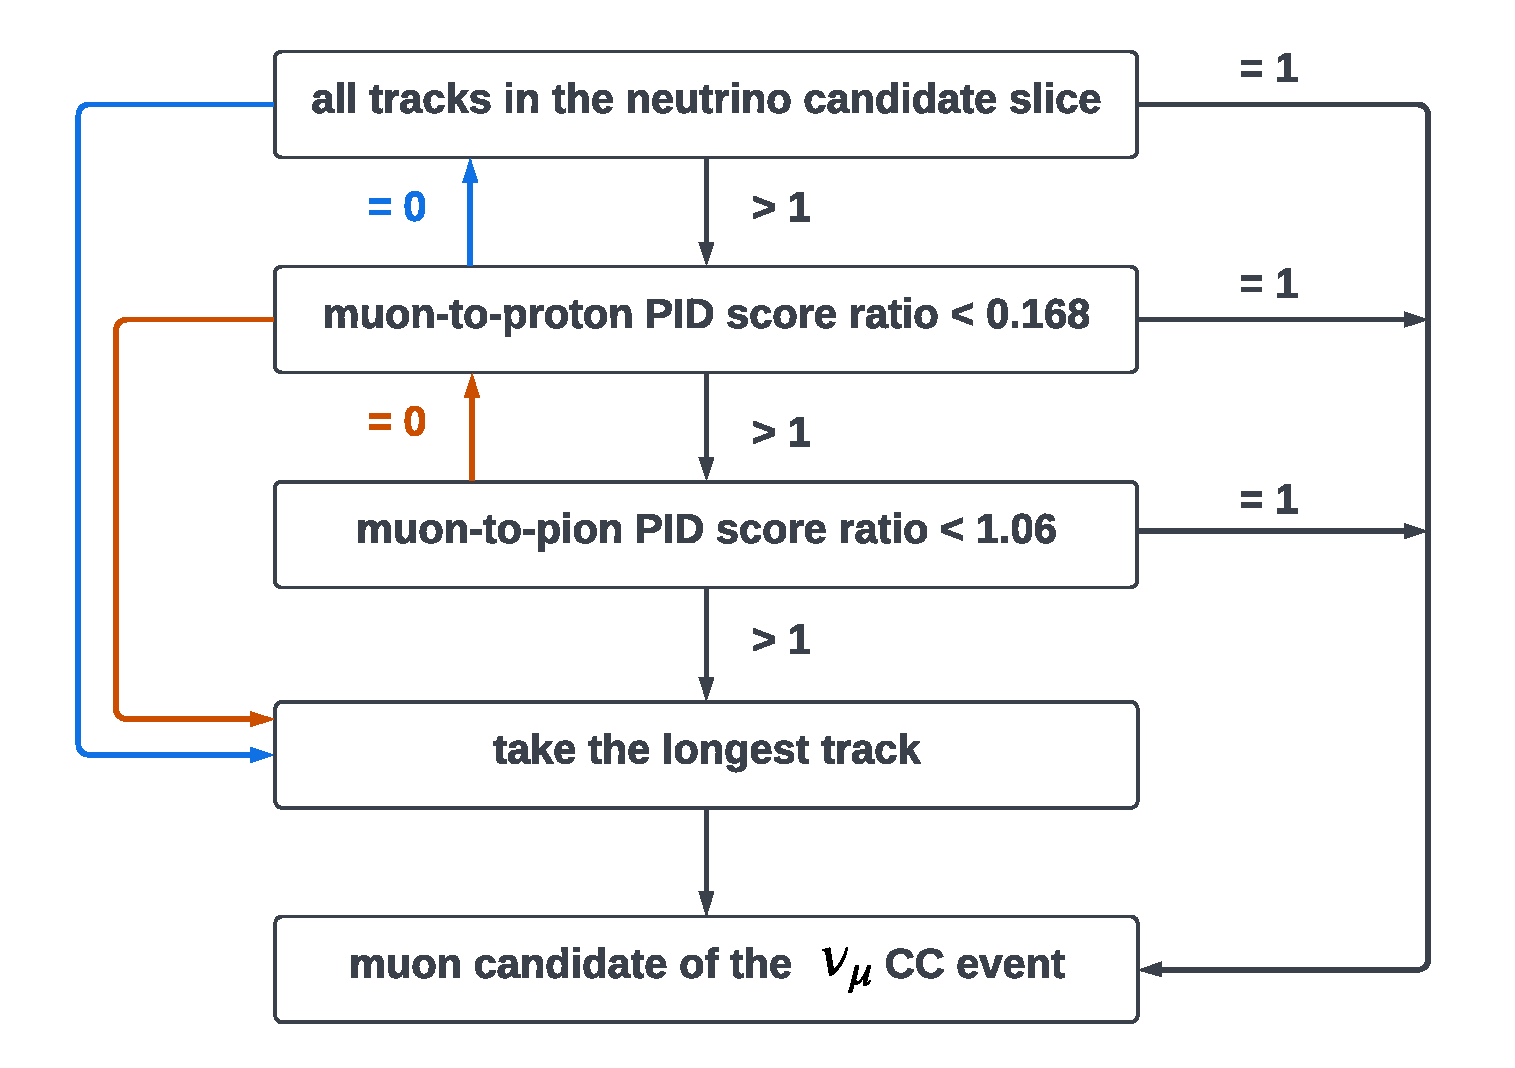
\includegraphics[width=0.8\textwidth]{images/NewCCInclusive/selection/muon_candidate_flow_chart.pdf}
  \caption[Moun Candidate Selection Flow Chart]{Shown above is a flow chart of the muon candidate selection. Listed in the Boxes, we finds the selection conditions. The numbers and relations ($=0$, $=1$, and $>1$) associated to the arrows, show the number of tracks fulfilling the selection conditions.}
  \label{fig:muon_candidate}
\end{figure}
An evaluation of above procedure using the $\nu_\mu$ \gls{cc} events of the \gls{bnb} overlay sample, shows that we are correctly identifying about \SI{97}{\percent} of the muon tracks with reconstructed lengths greater than \SI{8}{\centi\metre}. The misidentified tracks are associated with pions by \SI{1.6}{\percent} and with protons by \SI{1.3}{\percent}.

% -------------------------------------------------------------------------------------------------------------------------------------------------------------------------------------------------------------------------------------

\subsection{Muon Neutrino Charged Current Inclusive Selection} \label{sec:NewNuMuCCSelection}
% TODO Find a place for this
% Therefore, the \gls{crt} is a powerful tool in removing such background, which can be concluded by comparing the selection purity of this analysis (\SI{72}{\percent}) and the one from the previous generation (\SI{50}{\percent}).
With the muon candidate selected, we can now focus on removing backgrounds from $\nu_{\mu}$ \gls{cc} inclusive events, \ie signal events, and aim to select a sample with high efficiency and purity. In correspondence to our signal definition, we also require the reconstructed neutrino \glspl{Vertex} to be in the \gls{fv} which is spatially calibrated using the \gls{lcs} and cosmic-ray muon tracks (for reference see \ref{sec:LaserCalibrationSystem} and \ref{sec:SpaceCharge}). For this purpose the apparent entry and exit points of the \gls{uv}-laser beams and the cosmic rays are used to determine the \gls{fv} which is warped by the space charge effect. In this sense, a track is labelled as contained if the track start is in the now warped \gls{fv} and the track end is within a boundary of \SI{5}{\centi\metre} to the apparent \gls{tpc} edge (containment volume). Concurrently, if a track features its start in the newly defined \gls{fv} and the track end outside of the containment volume, the track is tagged as uncontained. 

The kinematic distributions of muon candidates with the above-described additional \gls{fv} cut applied are shown in figure \ref{fig:PreselectionDistributions}.
\begin{figure}[htbp]
	\begin{center} \centering
		\subfloat[Muon momentum]
        {
            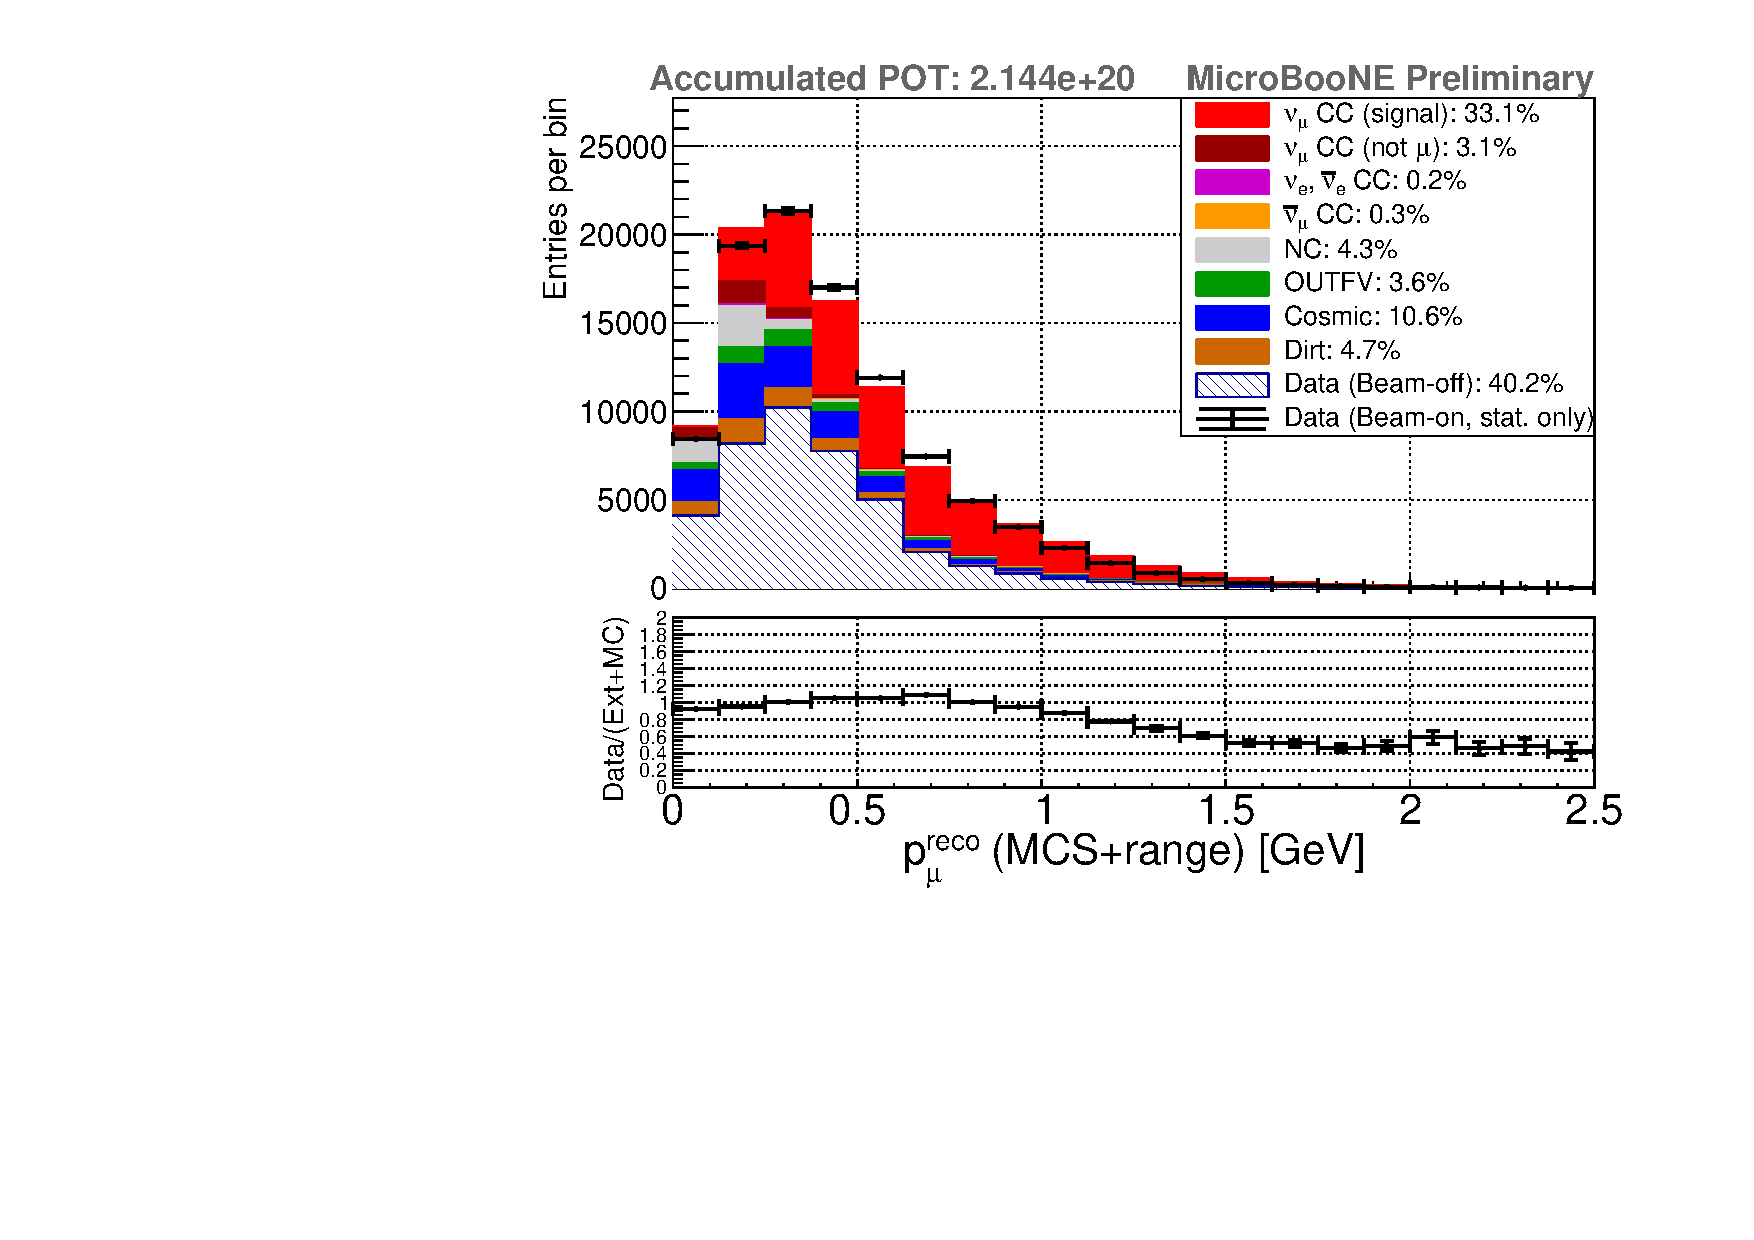
\includegraphics[width=0.49\textwidth]{images/NewCCInclusive/selection/TrackMCSRange_01.pdf}
            \label{fig:muon_momentum_before_cuts}
        }
		\subfloat[Muon cos($\theta$)]
        {
            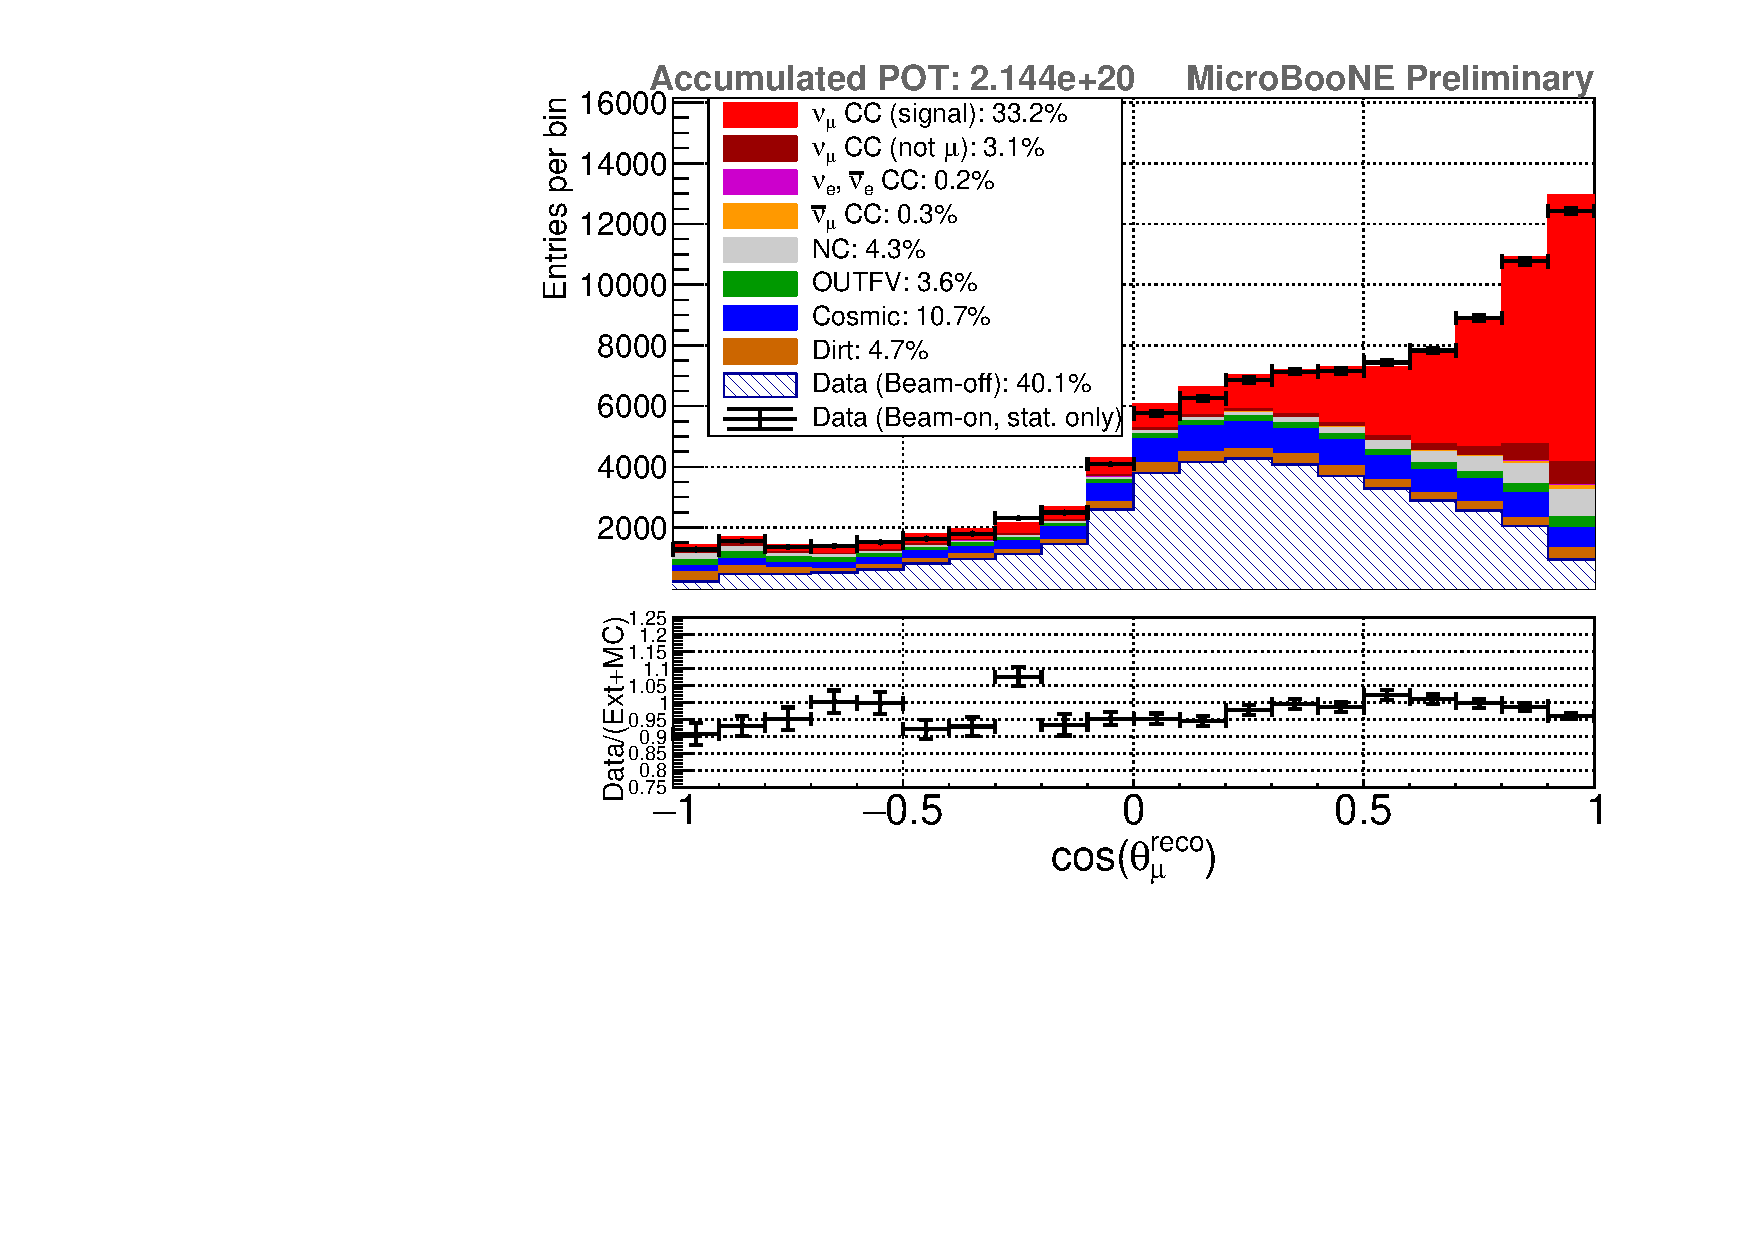
\includegraphics[width=0.49\textwidth]{images/NewCCInclusive/selection/cosTheta_01.pdf}
            \label{fig:muon_costheta_before_cuts}
        } 
        \caption[Muon Candidate Momentum and $\cos{(\theta)}$ Distributions after Pre-Selection]{Depicted above are the kinematic distributions of the muon candidates' momentum in \subref{fig:muon_momentum_before_cuts} and their $\cos{(\theta)}$ in \subref{fig:muon_costheta_before_cuts}, both after applying the spatially calibrated \gls{fv} cut. The momentum reconstruction uses the \gls{mcs} method as well as \gls{csda} for contained tracks. The \gls{tpc} data is indicated in black while the \gls{mc} truth signal is drawn as a bar diagram in red, stacked on top of different groups of background interactions are listed (see beginning of Section \ref{sec:NewEventSelection}).} 
        \label{fig:PreselectionDistributions}
	\end{center}
\end{figure}
As the forward-folded cross section of $\nu_{\mu}$ \gls{cc} interactions is presented as a function of reconstructed muon momentum and muon $\cos{(\theta)}$, it is useful to monitor these two muon kinematic distributions. At this stage, the purity of the sample is \SI{30}{\percent}, and the dominant background is cosmic induced (mainly from Beam off) which at this point makes up more than \SI{50}{\percent} of the sample. Moreover, it is notable, that the backgrounds are mostly located in the lower end of the reconstructed muon momentum distribution. In the $\theta$-angle picture, the majority of the signal events are pointing in the direction of the beam vector, \ie $\cos{(\theta)}\sim 1$ and generally $\cos{(\theta)} > 0$. Meanwhile, the cosmic background events seem to have a more vertical character with a maximum at $\sim\SI{70}{\degree}$, or $\cos{(\theta)}\sim \num{0.3}$, which is expected for distributions without a $d\Omega$ parametrisation (see section \ref{sec:CosmicRayTheory}). The $\nu_{\mu}$ \gls{cc} (unmatched $\mu$) background is about \SI{10}{\percent} of the $\nu_{\mu}$ \gls{cc} signal which is seemingly worse than the performance stated in section \ref{sec:NewMuonCandidateSelection}. However, this could be caused by the fact, that some of neutrino slices may not include a muon track which suffuses the truth matching criteria (containing more than half of the true muon energy).

Given the dominant cosmic-ray induced background, it seems beneficial to make use of the \gls{crt} information to reduce the cosmic contamination. As the top \gls{crt} plane is \SI{5}{\metre} above the \gls{tpc}, in order to accommodate the detector racks for systems such as the high voltage and data acquisition (see section \ref{sec:CRT}), neutrino induced particles rarely hit the top \gls{crt} plane, particularly at \gls{bnb} energies. Most neutrino events Furthermore, with the large gap, said plane also features small angular acceptance for neutrino induced particles. On the contrary, cosmic-ray induced particles are mostly downwards-going, and are therefore very likely to be tagged by the top \gls{crt} plane. Hence, we select the events with no \gls{crt} hits in the top plane during the beam window. Figure \ref{fig:no_top_CRT_cut1} shows the number of \gls{crt} hits in the top \gls{crt} plane which verifies that most of the neutrino interactions have no \gls{crt} hits in the top planes within the beam window but many cosmic events do. We dare speculate, that the few signal events removed by this cut, are in coincidence with cosmic-ray hitting the top plane within the beam window time frame.
\begin{figure}[htbp]
  \centering
  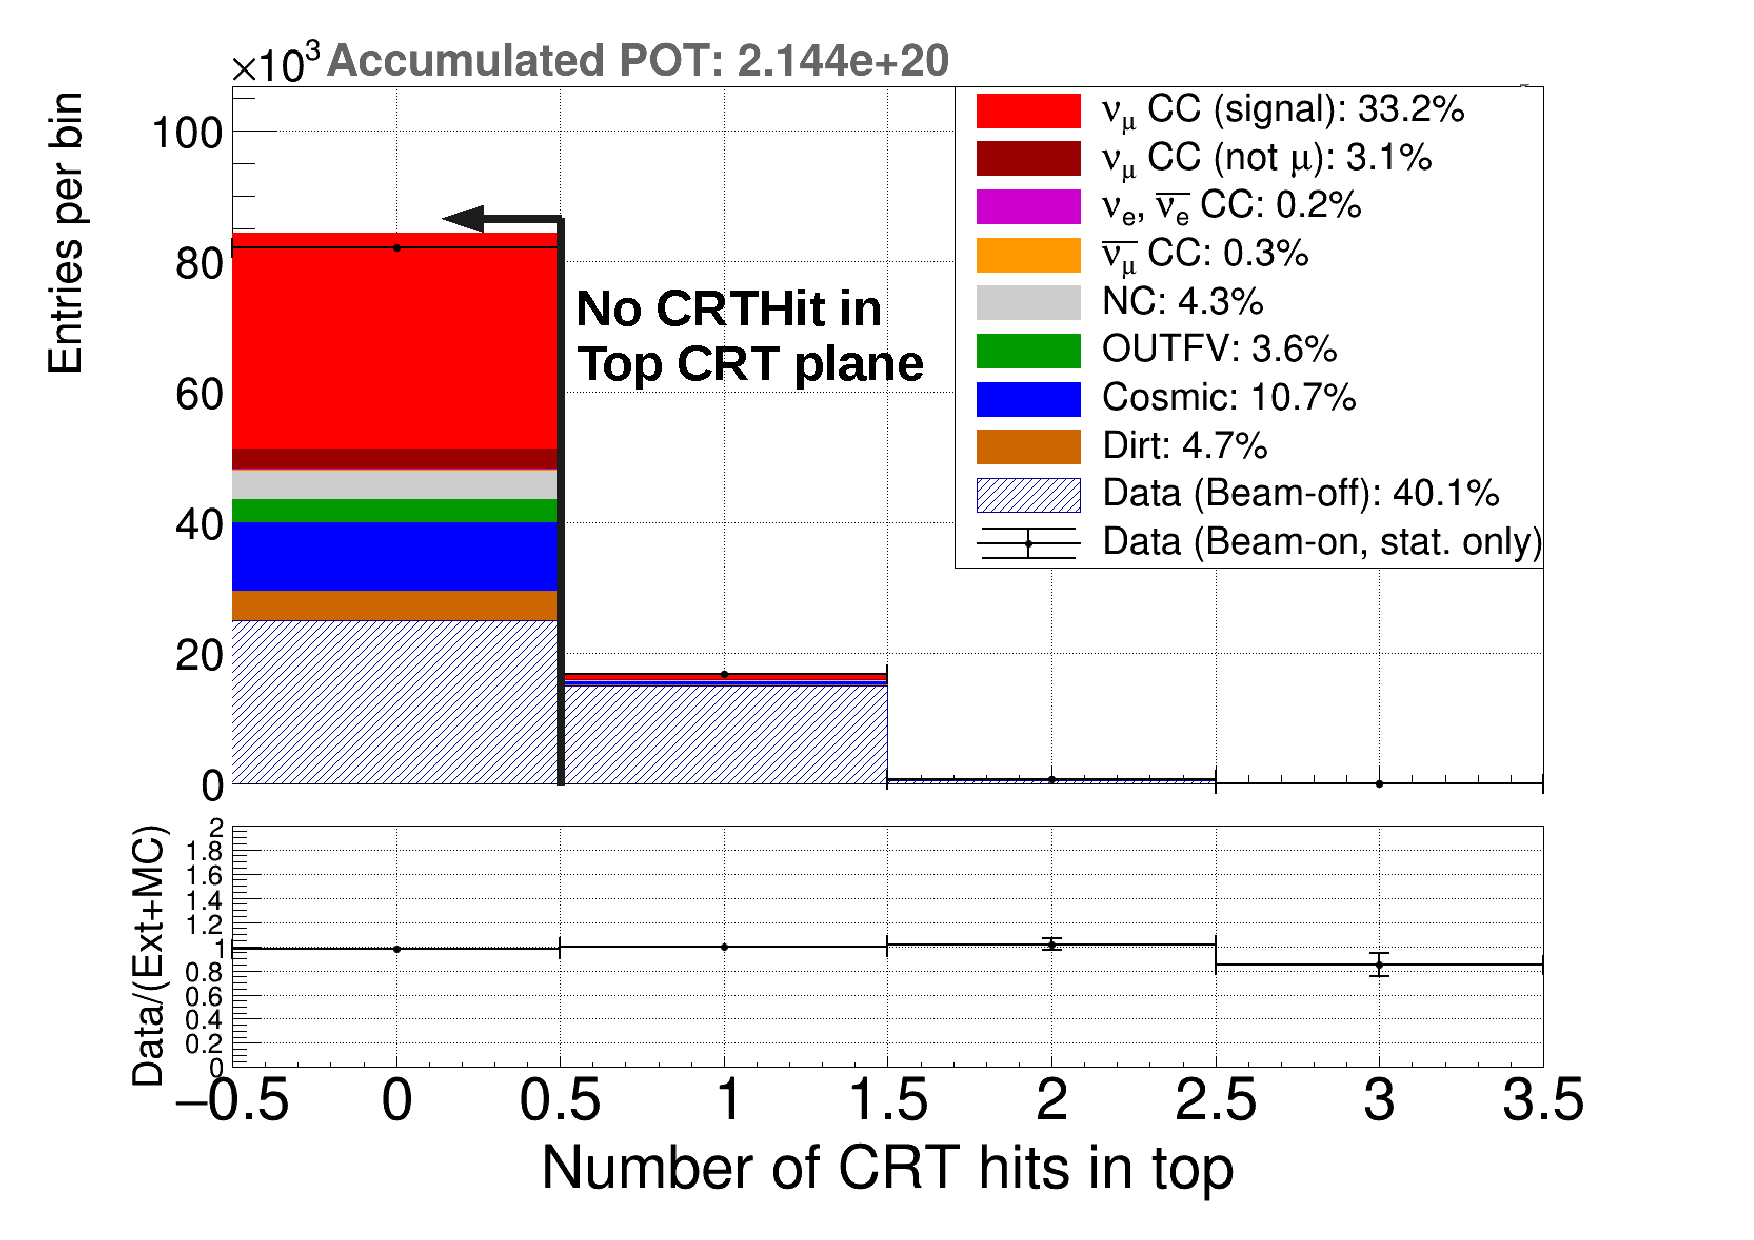
\includegraphics[width=0.7\textwidth]{images/NewCCInclusive/selection/No_CRThit_top_1.pdf}
  \caption[CRT Top Plane Cut]{Number of \gls{crt} hits in the top \gls{crt} planes during the beam window.}
  \label{fig:no_top_CRT_cut1}
\end{figure}

With the \gls{bnb} neutrino energies, we expect most muons produced in $\nu_{\mu}$ \gls{cc} interactions to be forward-going (see figure \ref{fig:muon_costheta_before_cuts}), and therefore the \gls{crt} hits, if there are any signal related ones, should be downstream to the neutrino \glspl{Vertex}. Neutrino interactions outside the \gls{tpc}, modelled by the dirt overlay sample, and cosmics, mainly modelled by the beam off sample, can be selected with the track ends wrongly reconstructed as a neutrino interaction \gls{Vertex}. We further investigated the properties of these misreconstructed \glspl{Vertex} and found a correlation between the distribution of the \gls{Vertex} to related \gls{crt} hit distance along the beam axis, \ie the $z$-coordinate in MicroBooNE (see figure \ref{fig:MicroBooNECoordinateSystem}), and their background origin. These correlations are presented in figure \ref{fig:posZ_CRT_cut2} which shows the differences of \gls{crt} hit positions and reconstructed neutrino \gls{Vertex} positions on the $z$-axis. This is done for the pure cosmic beam off sample (green), \gls{bnb} overlay with neutrino events only (red) and dirt overlay (blue) samples, all without any $\nu_{\mu}$ \gls{cc} selection cuts. 
\begin{figure}[htbp]
  \centering
  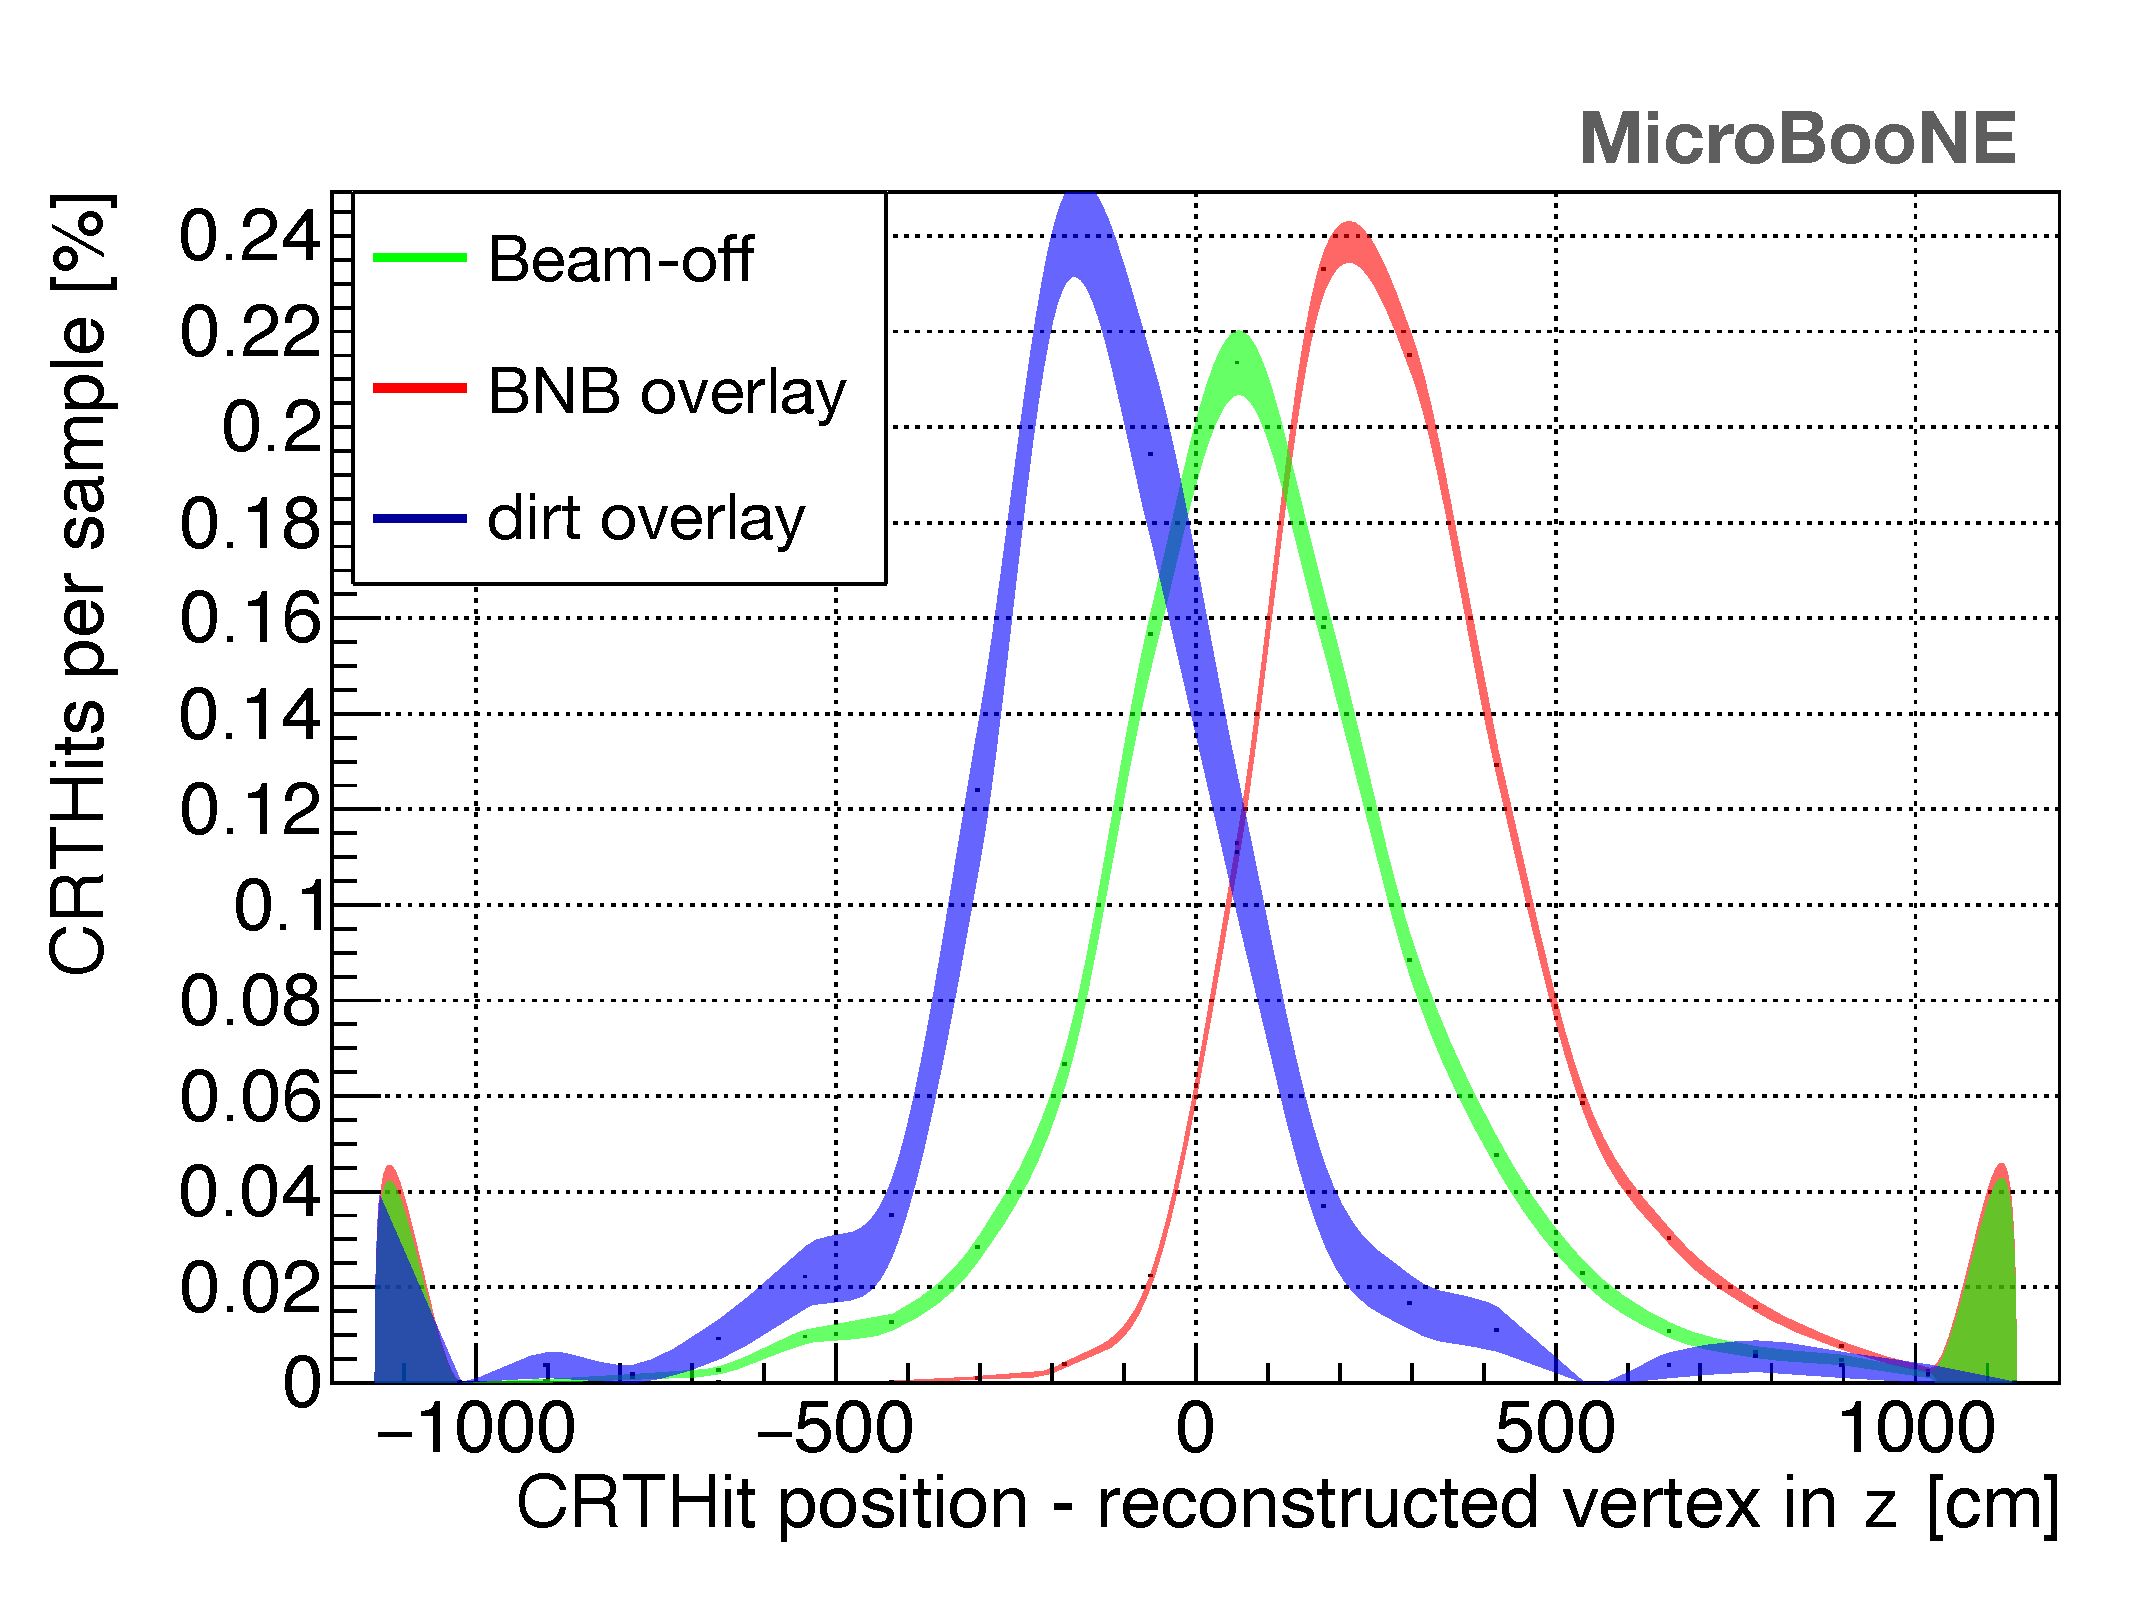
\includegraphics[width=0.7\linewidth]{images/NewCCInclusive/selection/posZ_CRT_vertex.pdf}
  \caption[Vertex to CRT Hit Distance for Multiple MC Samples]{The green, red and blue histograms show the normalised distributions of the position differences between \gls{crt} hits and reconstructed primary \glspl{Vertex} along the beam direction. Green represents the beam off, red the \gls{bnb} overlay without cosmics, and blue the dirt overlay samples, respectively. All curves are normalised to their integral, and the line width represents the statistical uncertainty of the respective distribution.}
  \label{fig:posZ_CRT_cut2}
\end{figure}
More specifically, the \gls{bnb} overlay (red) and the dirt overlay (blue) distributions only contain the simulation part of the overlay samples, while the beam off (green) distribution stems from measured cosmic-ray data. Each distribution is normalised to show the relative percentage within the sample, and the vertical band indicates the statistical uncertainties. As can be seen, a vast majority of the \gls{crt} hits from neutrino interactions in the \gls{bnb} overlay sample are downstream of the reconstructed neutrino vertex, as expected for a properly reconstructed \gls{Vertex}. The misreconstructed \glspl{Vertex} of the beam off and dirt overlay samples, however, allow for more upstream \gls{crt} hits as seen in the graph. This is especially true for events of the dirt overlay sample, which feature most of their true \glspl{Vertex} upstream of the \gls{tpc}. As the cosmic muons mainly travel downwards, the green distribution is not significantly biased towards either the positive nor the negative side.

From this, we derived our next selection step which disallows any \gls{crt} hit upstream of the reconstructed neutrino \gls{Vertex} during during the beam window. The result of this selection is depicted in figure \ref{fig:no_upstream_CRT_cut2} showing the number of \gls{crt} hits that are in the beam window and upstream to the reconstructed neutrino \gls{Vertex}.
We remove events with any \gls{crt} hits upstream to the reconstructed neutrino \gls{Vertex} in the beam window which are mainly Comic and Dirt.
\begin{figure}[htbp]
  \centering
  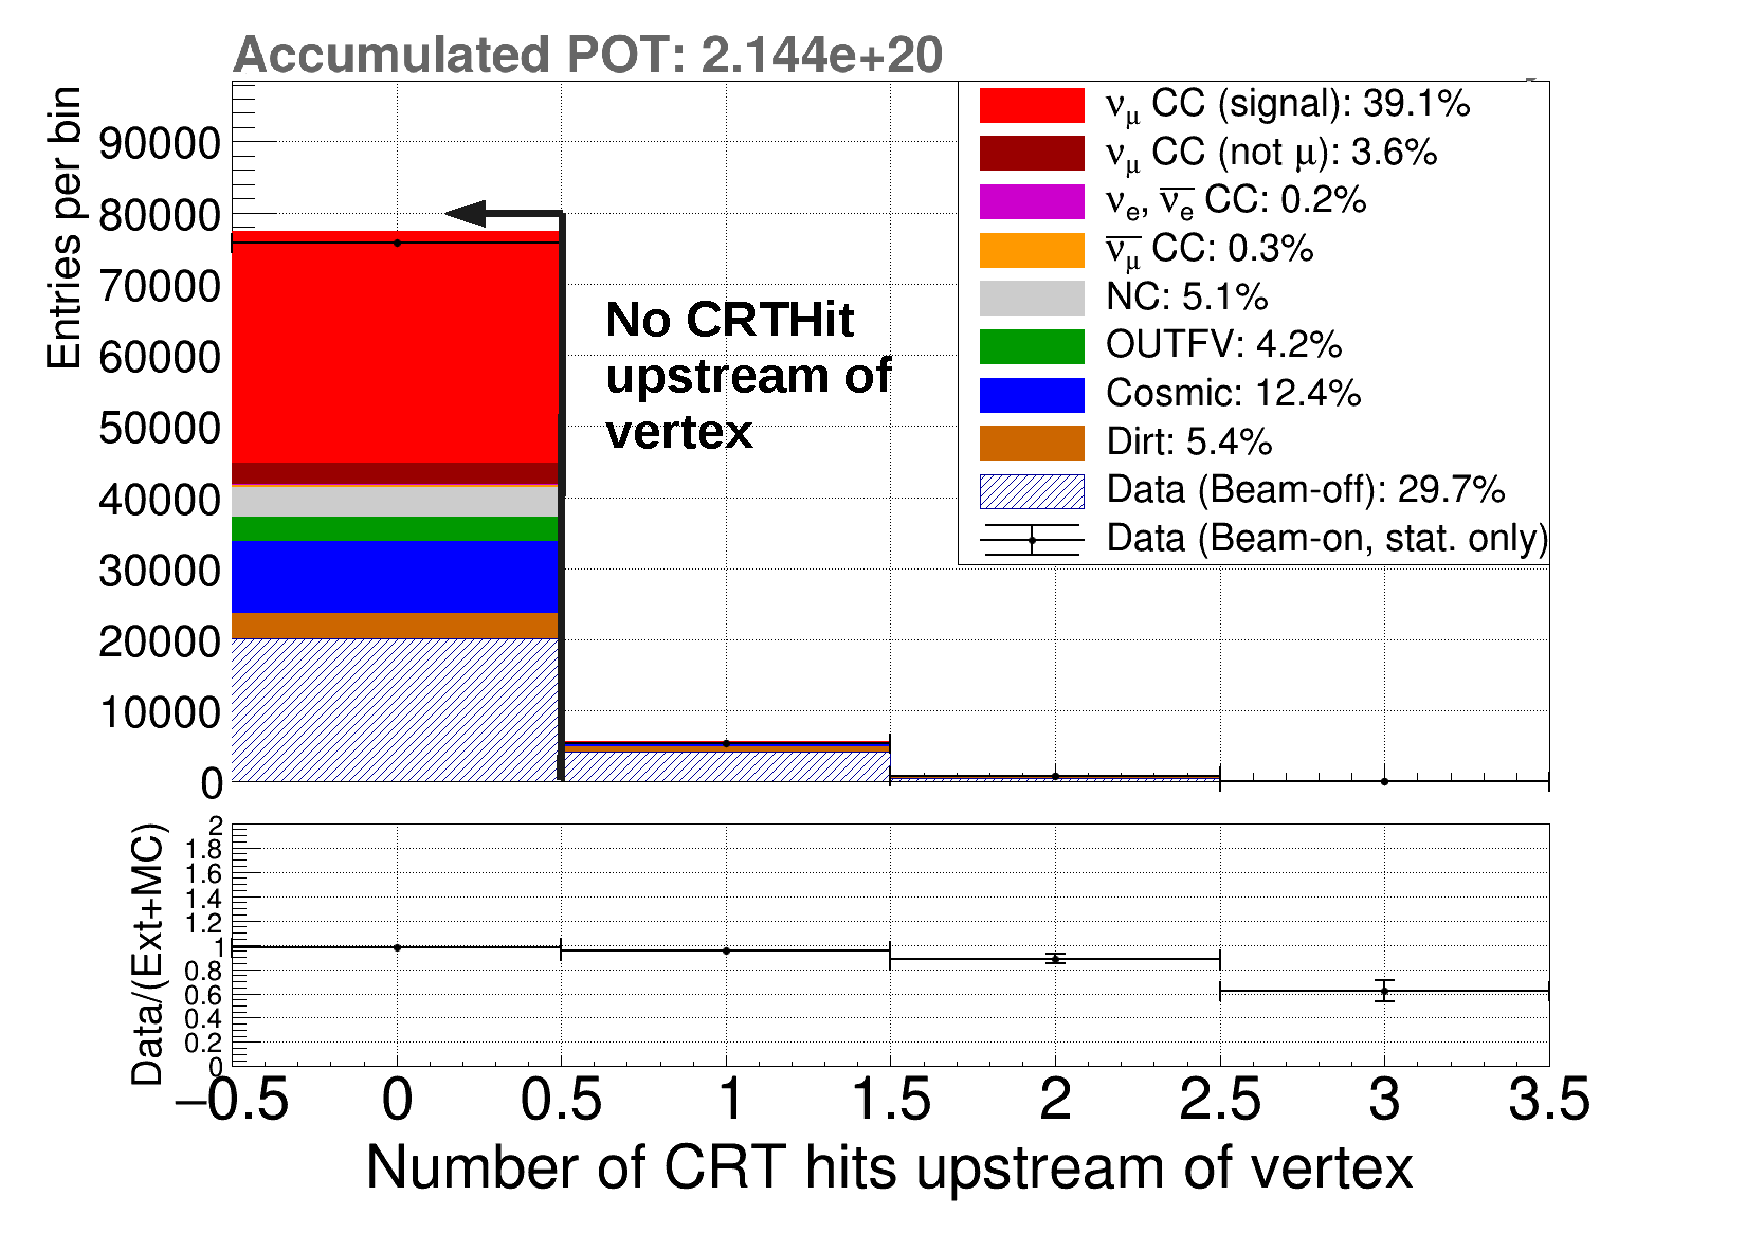
\includegraphics[width=0.7\textwidth]{images/NewCCInclusive/selection/No_upstream_CRT_2.pdf}
  \caption[CRT hit Upstream of Vertex Cut]{Number of \gls{crt} hits within the beam window which are upstream in the \gls{bnb} direction with respect to the reconstructed neutrino \gls{Vertex}.}
  \label{fig:no_upstream_CRT_cut2}
\end{figure}

In the next selection step, we expand above logic of excluding background-prone \gls{crt} hit patterns to neutrino interaction events contained in the active volume. As it is difficult to ensure full containment from reconstructed slices alone, we use the muon track as a proxy, for it is usually the most spatially expansive object. Furthermore, hadrons from the same interaction likely lose all their kinetic energy within the cryostat volume, typically featuring a \SI{1.5}{\metre} long column of \gls{lar}, before they can reach any \gls{crt} plane. Hence, if the muon originating from a $\nu_{\mu}$ \gls{cc} interaction is contained, we veto events with any \gls{crt} hits within the beam window. Figure \ref{fig:no_CRThits_contained_3} shows the composition of vetoed and non-vetoed events. Note that the non-vetoed events also include all uncontained muon events.
\begin{figure}[htbp]
  \centering
  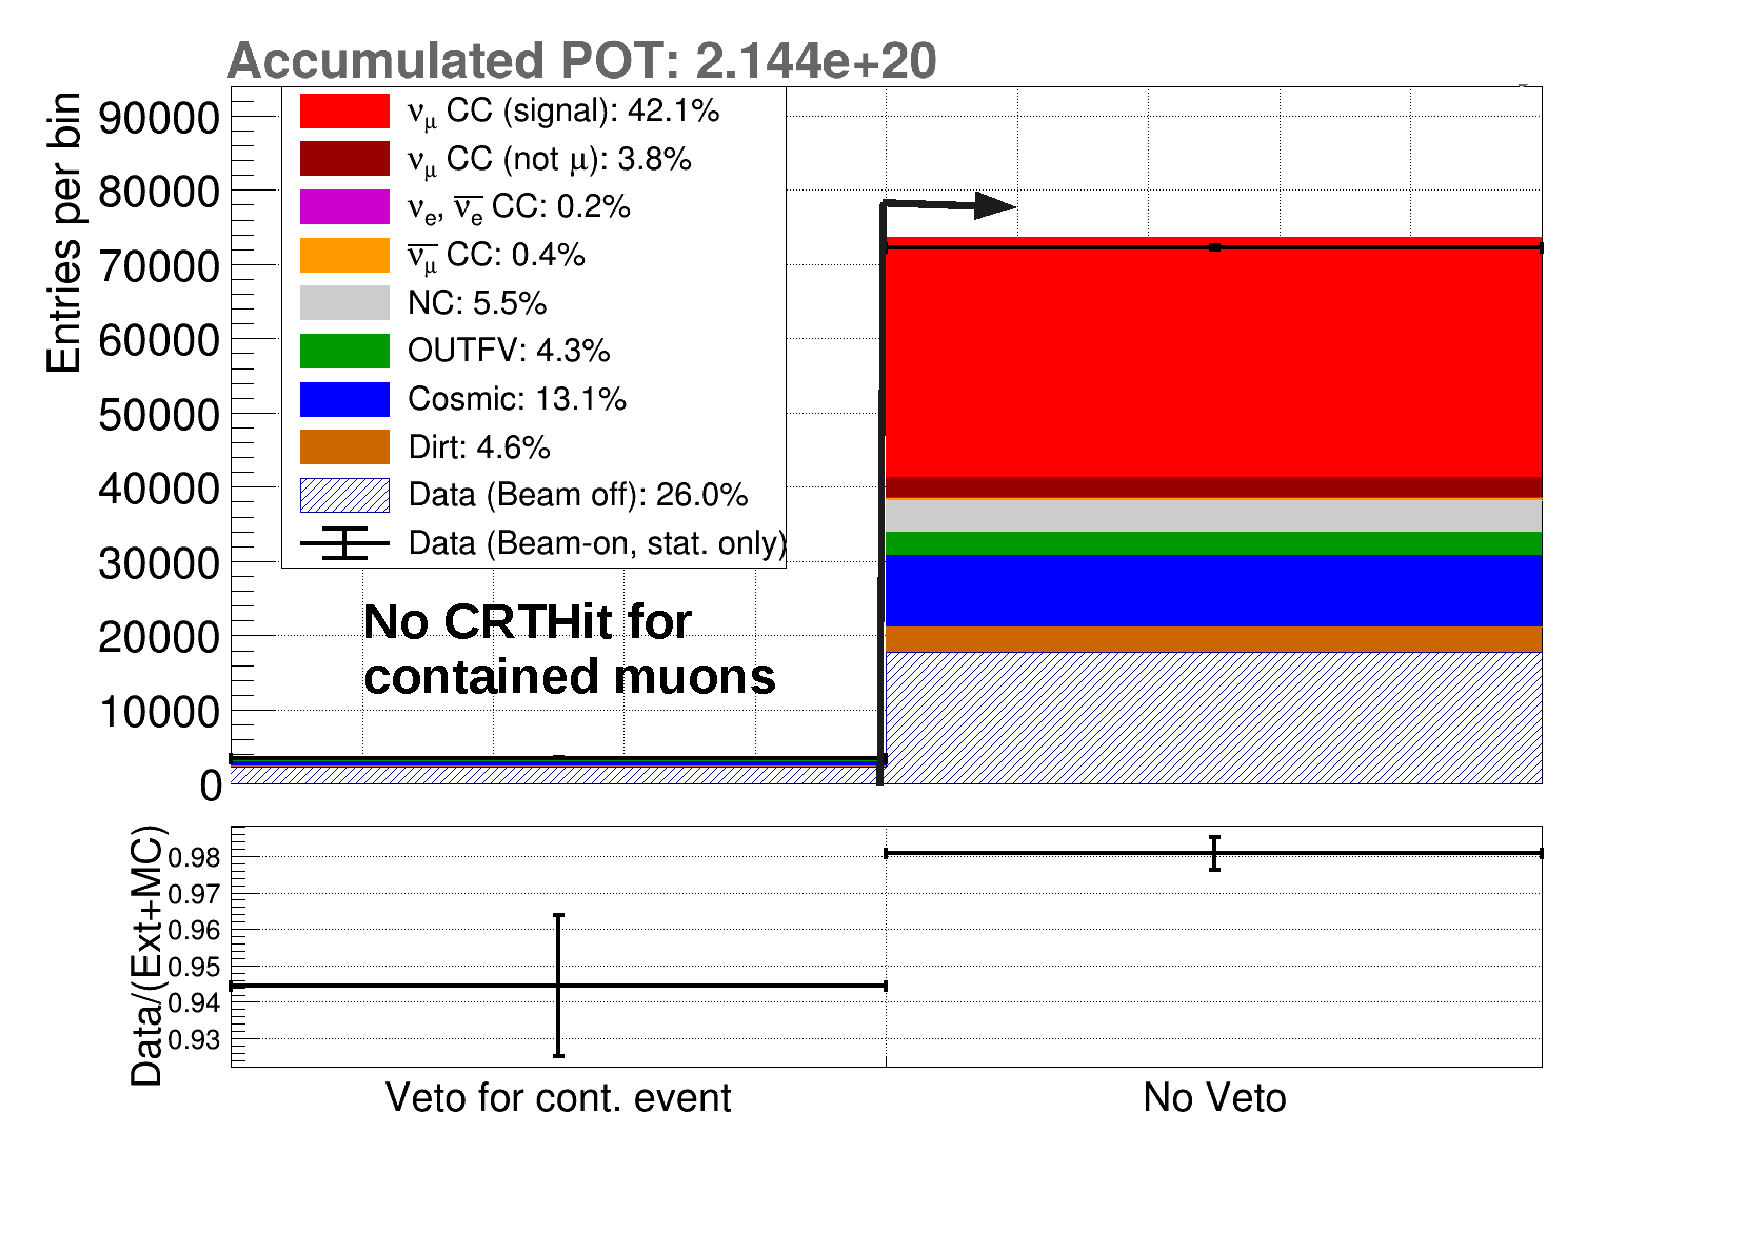
\includegraphics[width=0.7\textwidth]{images/NewCCInclusive/selection/No_CRThits_contained_3.pdf}
  \caption[CRT Veto on Contained Muons]{The graph above shows contained muon \gls{crt} veto effectiveness. The veto condition does not allow contained muon in coincidence with any \gls{crt} hits in coincidence with the flash associated to the neutrino slice. The composition of vetoed events is found in the left bin and all remaining events are in the right bin.}
  \label{fig:no_CRThits_contained_3}
\end{figure}
% TODO Check if the crt hit is associatd to the flash duration (8us), or the beam window (1.6us)?

To conclude \gls{crt} related selection criteria, the cosmic-ray pileup matching is applied. The method of the associated drifted in cosmic signatures with \gls{crt} hits is already discussed in detail in section \ref{sec:CosmicPileupReduction} and schematically depicted in figure \ref{fig:CRTTrackAssociation}. So, all the muon tracks are geometrically matched with all the available \gls{crt} hits in the reconstruction stage. If the muon candidate track is associated to a \gls{crt} hit which is out of beam window, then this event is assumed to be of cosmic origin. The summary of this selection step is shown in figure \ref{fig:no_out_of_time_CRT_4}.
\begin{figure}[htbp]
  \centering
  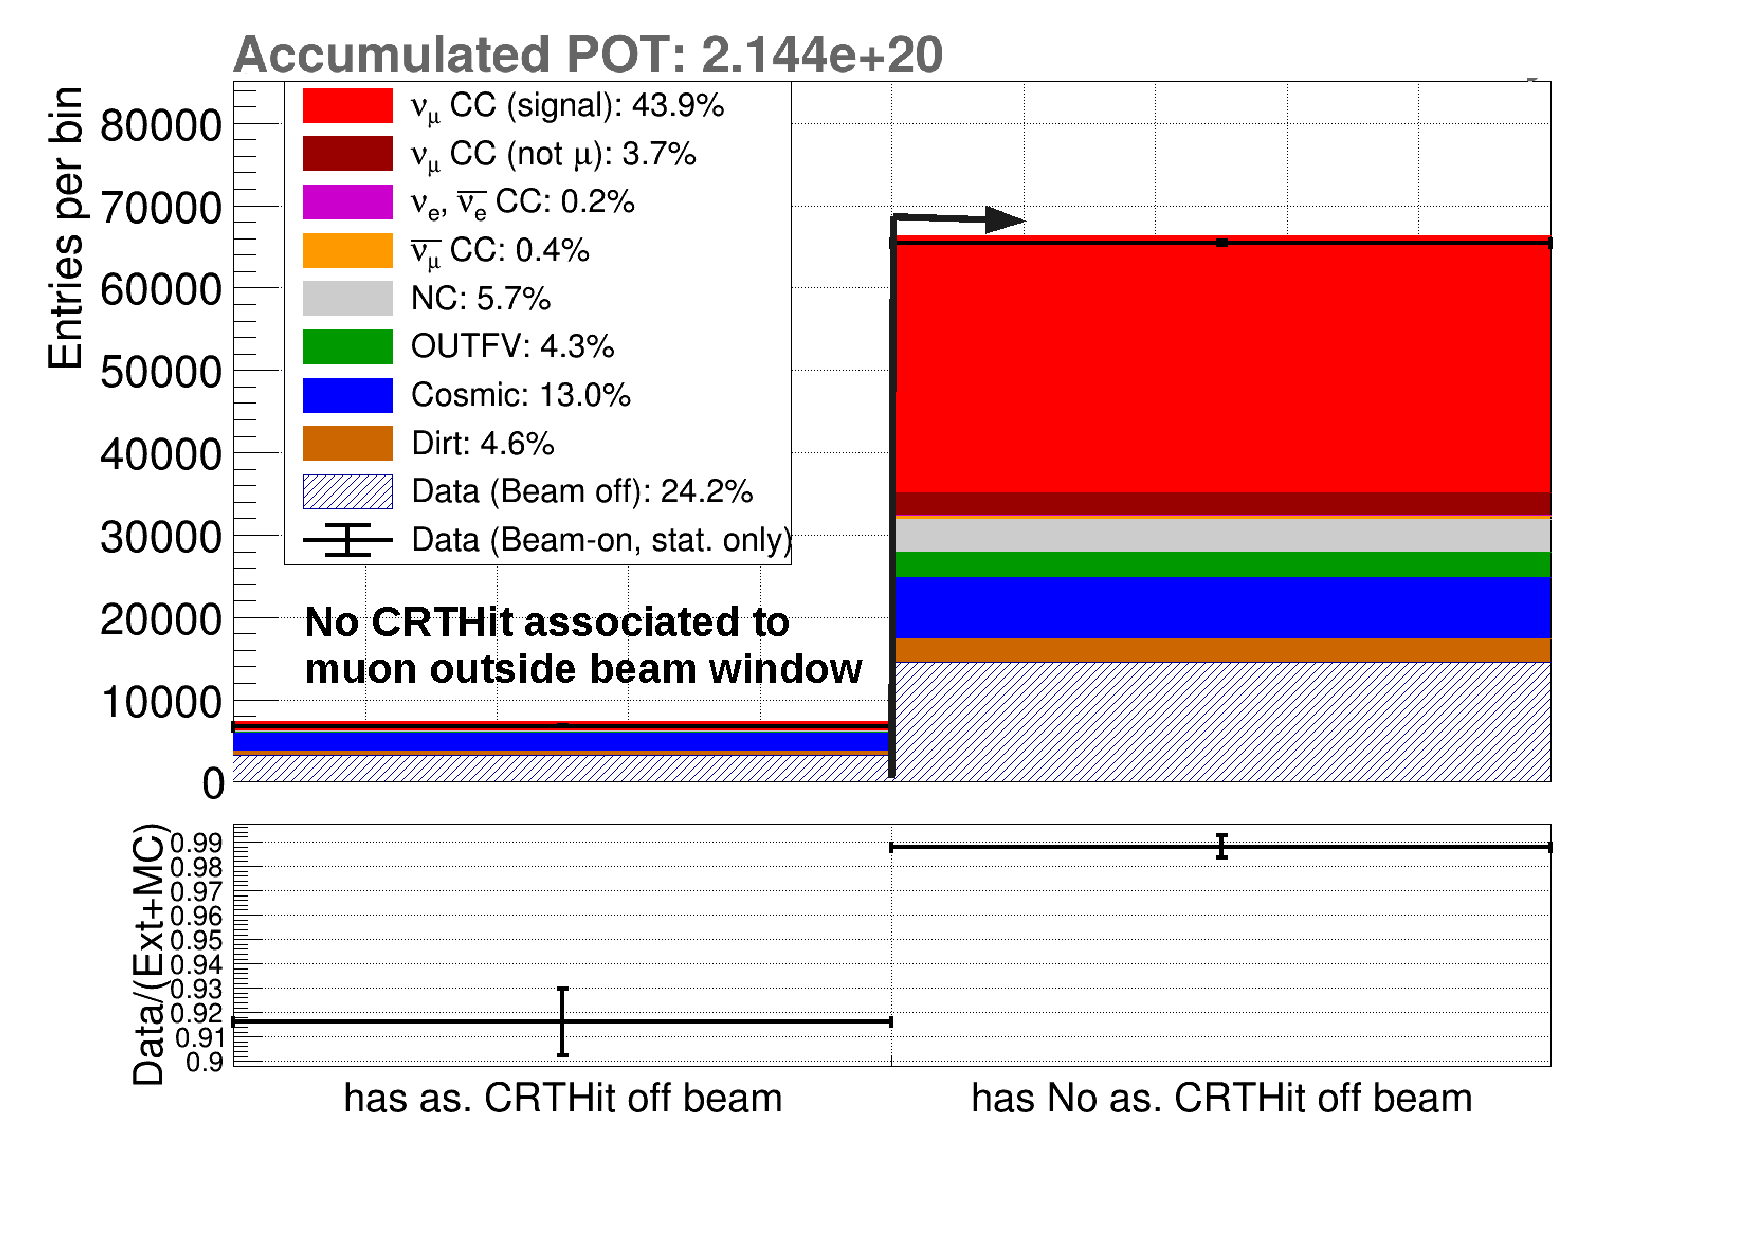
\includegraphics[width=0.7\textwidth]{images/NewCCInclusive/selection/No_out_of_time_CRT_4.pdf}
  \caption[CRT Hit Association Veto]{The muon candidates with associated \gls{crt} hits which are outside of the beam window are in the left bin, and the rest of the events are in the right bin.}
  \label{fig:no_out_of_time_CRT_4}
\end{figure}
As can be observed by the low amount of dropped signal events, a mismatch of the muon candidate to an out-of-beam-window \gls{crt} hit is rather rare. This speaks for the high reliability of this method, especially for future detectors, which are designed with better \gls{crt} coverage than MicroBooNE.

With all the \gls{crt} related selection cuts applied, the signal purity reaches \SI{47}{\percent}. But in order to further improve the selection, we intend to enforce even higher track quality control for the muon candidates. For this we utilise the track score produced by \gls{Pandora} using an \gls{svm}, as introduced in section \ref{sec:NewReconstruction}. In the next selection step, we require muon candidate tracks to exhibit a track score greater than \num{0.8}, instead of the default track definition value of \num{0.5}. Figure \ref{fig:trackscore_08_5} shows the track score distribution of the muon candidate tracks.
\begin{figure}[htbp]
  \centering
  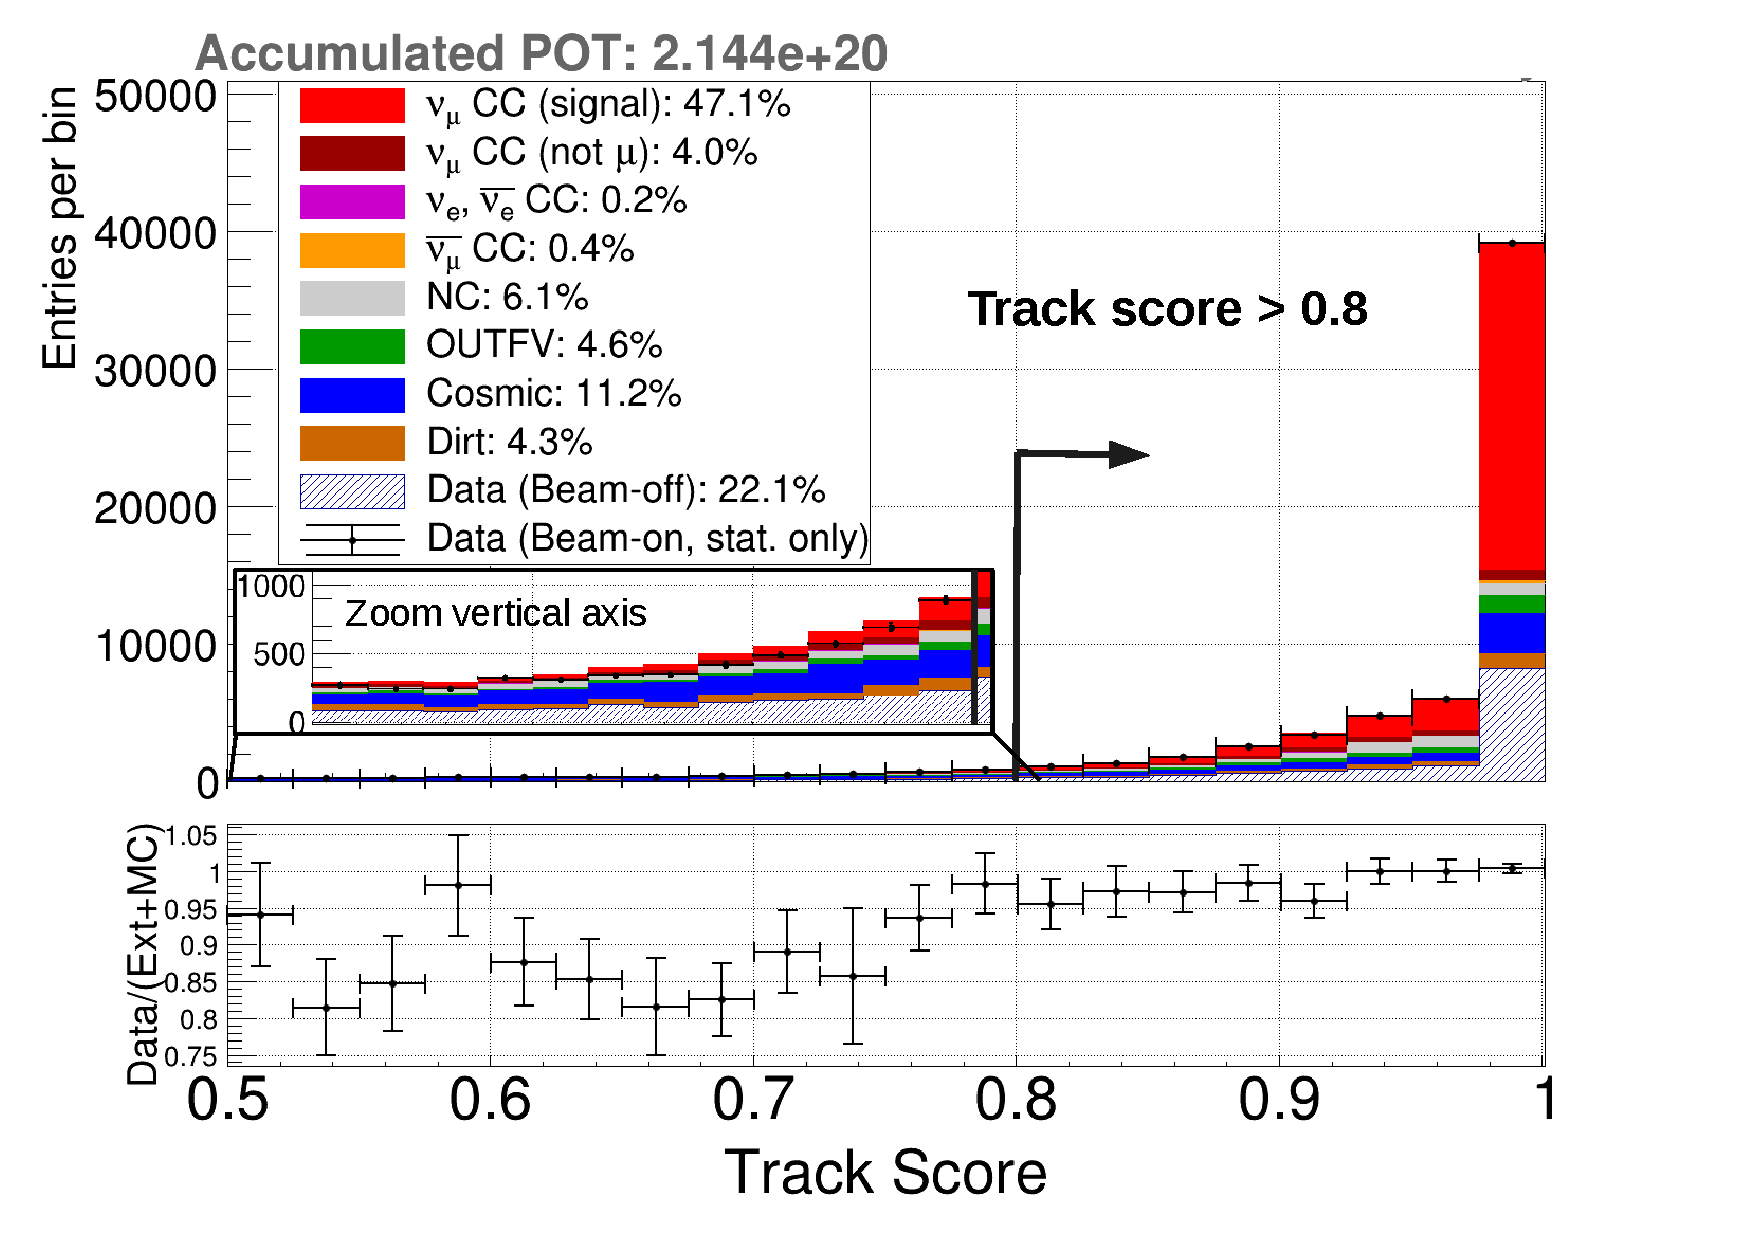
\includegraphics[width=0.7\textwidth]{images/NewCCInclusive/selection/Trackscore_08_5.pdf}
  \caption[Muon Candidate Track Score Cut]{The selected muon candidates are required to have track scores above 0.8.}
  \label{fig:trackscore_08_5}
\end{figure}

When considering the distribution of the muon candidates' track lengths, as depicted in figure~\ref{fig:track_length_20_6}, we observe that shorter tracks are dominated by backgrounds.
\begin{figure}[htbp]
  \centering
  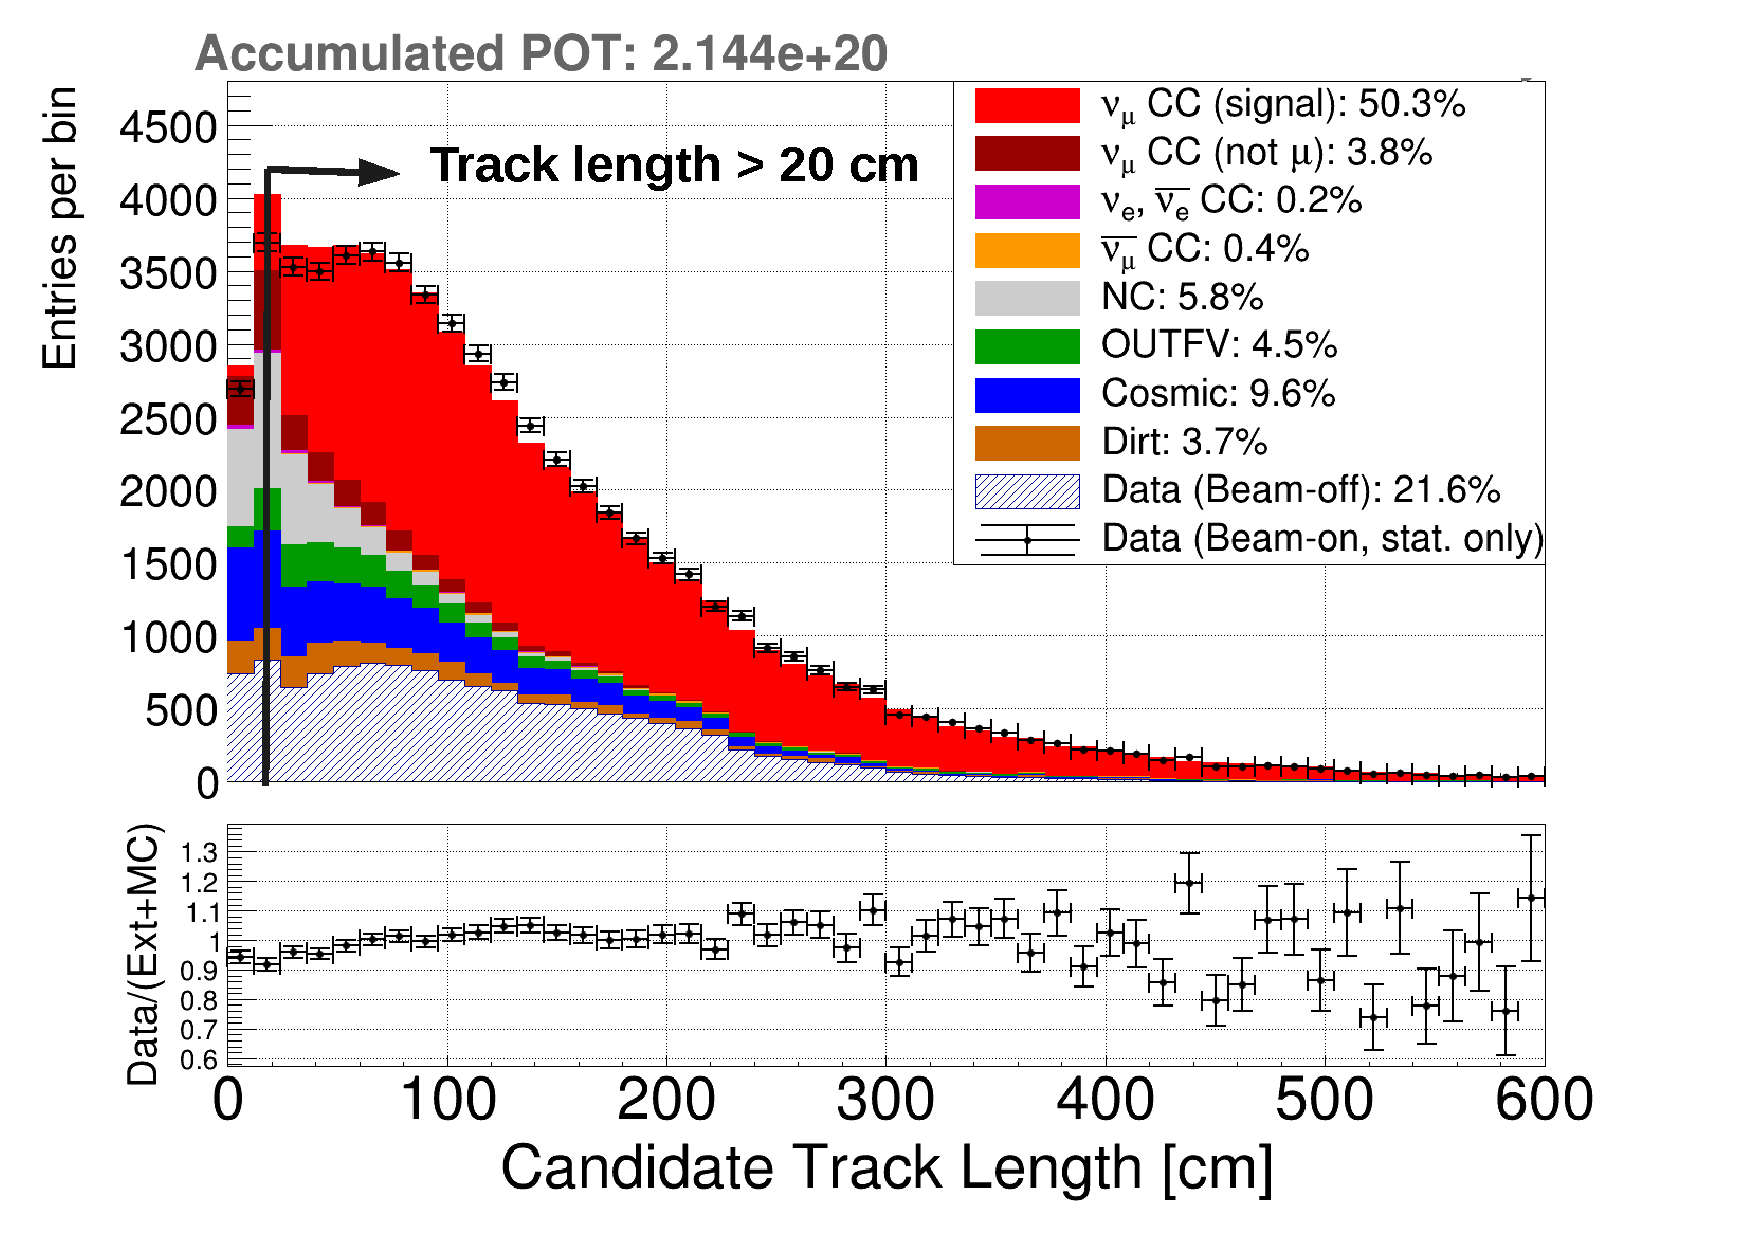
\includegraphics[width=0.7\textwidth]{images/NewCCInclusive/selection/Track_length_20_6.pdf}
  \caption[Muon Candidate Track Length Cut]{The distribution of the muon candidate track length. Since the shorter tracks are mainly background originated, we only select events with the muon candidate track longer than \SI{20}{\cm}.}
  \label{fig:track_length_20_6}
\end{figure} 
The most prominent group of backgrounds in these lower bins are the ones which feature their true \gls{Vertex} outside of the \gls{fv}, \ie cosmic pileup, beam off, dirt and ``out of \gls{fv}'' events. They are either detached traces of the same particle or reconstructed with a flipped directionality. With this, they are more likely to feature shorter tracks. In the second, less prominent group, are background neutrino interactions, especially \gls{nc} and $\nu_{\mu}$ \gls{cc} with a misidentified muon track. In both cases, we are looking at hadron tracks, which are generally shorter than muon tracks. Consequently, we select events featuring a muon candidate track longer than \SI{20}{\cm}, as shown in figure \ref{fig:track_length_20_6} above.

Until this point, we used the most muon-like track as every event's muon candidate, see section \ref{sec:NewMuonCandidateSelection}. Now, we utilise the then used \gls{pid} $\chi^2$ to introduce a \gls{pid} selection cut. More specifically, we are using the $\chi^2$ score for the proton hypothesis. The distribution of said score for the remaining muon candidate tracks is displayed in figure \ref{fig:PID_proton_78_7}.
\begin{figure}[htbp]
  \centering
  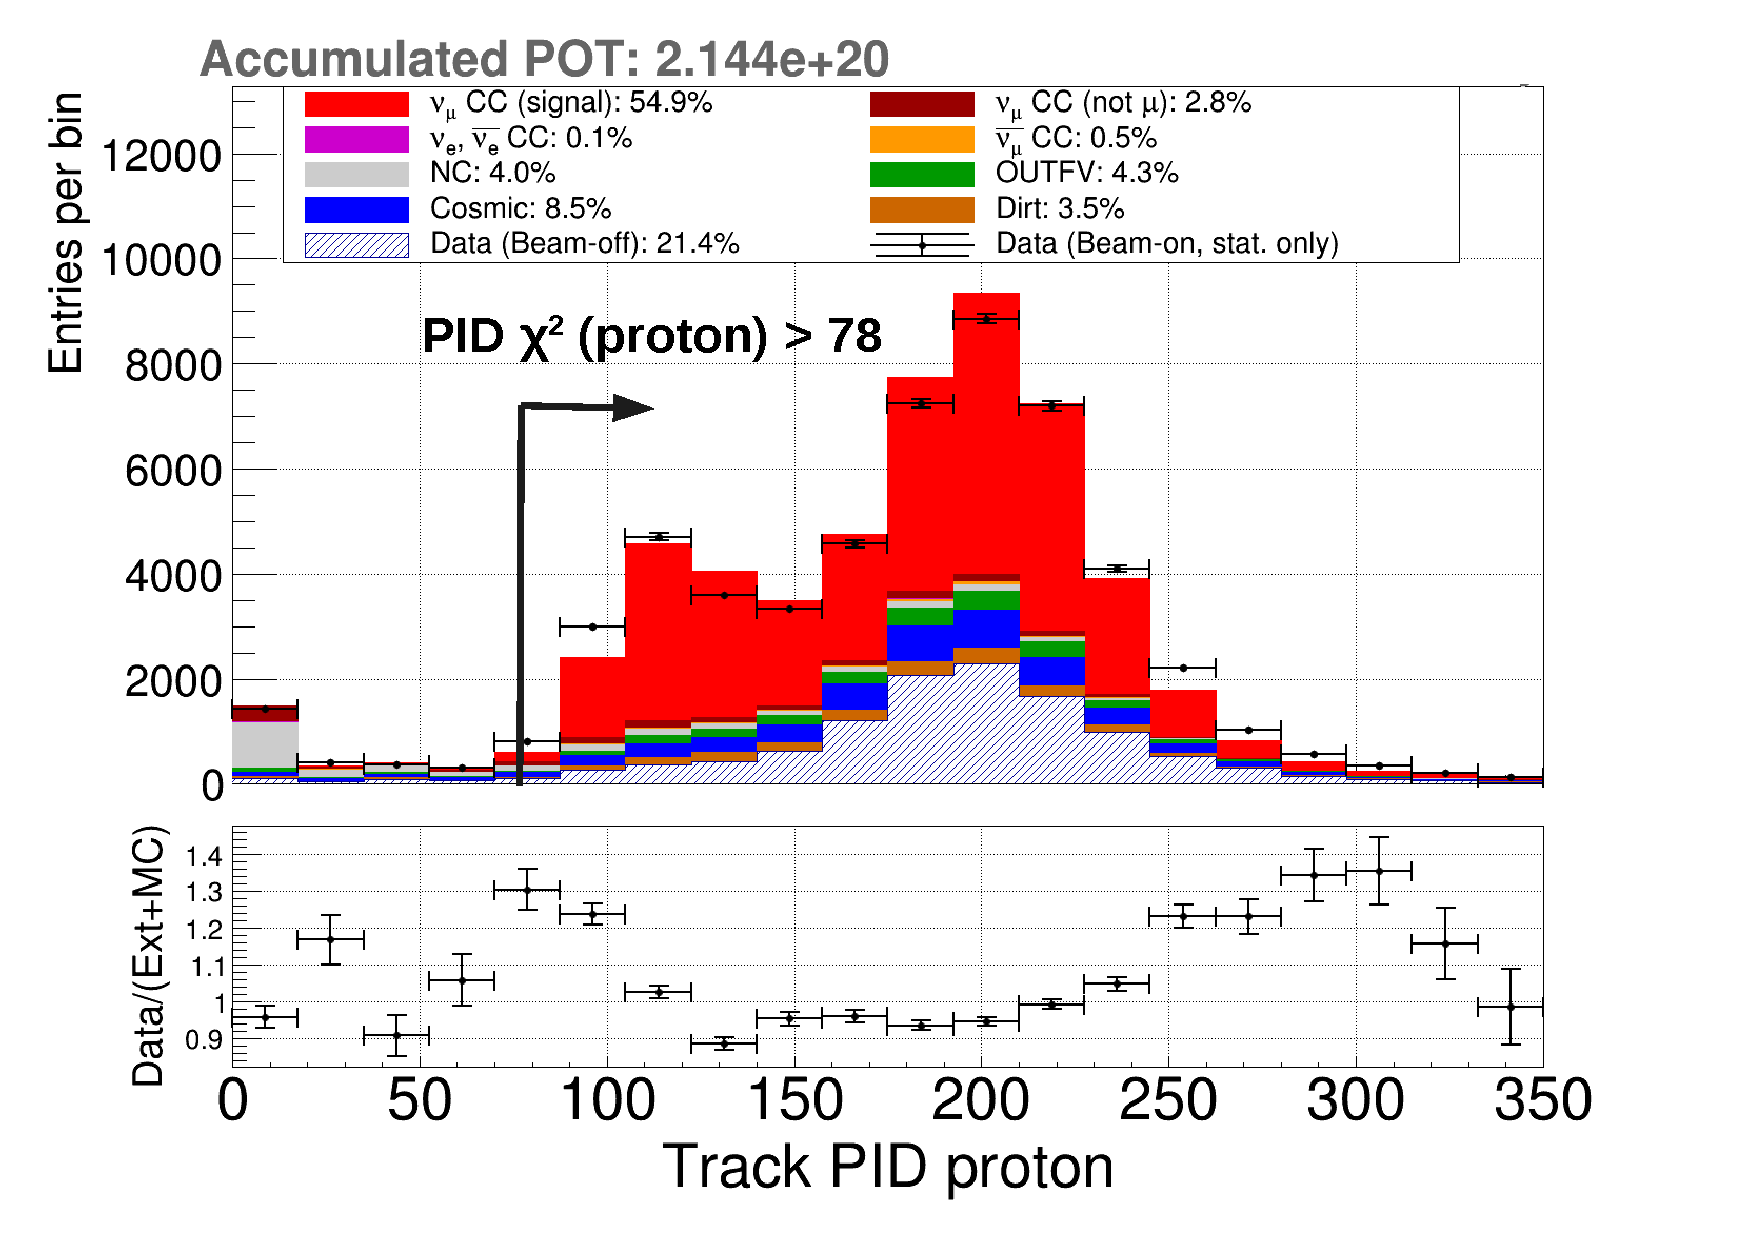
\includegraphics[width=0.7\textwidth]{images/NewCCInclusive/selection/PID_proton_78_7.pdf}
  \caption[Muon Candidate PID Chi-Square Cut]{The distribution of \gls{pid} $\chi^2$ scores with proton hypothesis. The events with \gls{pid} $\chi^2$ scores greater than \num{78} for the muon candidate tracks are selected.}
  \label{fig:PID_proton_78_7}
\end{figure}
The proton hypothesis gives the best separation power between protons and \glspl{mip}, \eg muons. The lower peak around zero in \gls{pid} $\chi^2$ (proton hypothesis) is dominated by backgrounds from \gls{nc} and $\nu_\mu$ \gls{cc} (unmatched $\mu$) which are mostly protons. For the selection, we require the muon candidate track to have \gls{pid} $\chi^2$ score (proton hypothesis) greater than \num{78} to remove proton-like tracks.

For the final selection step, we review topological scores of the selected neutrino slices, as shown in figure \ref{fig:topological_score_01_8}. The topological score is a convoluted discriminator for cosmic and neutrino events using charge information in the slice (see section \ref{sec:NewReconstruction} for more context). Cosmic-ray induced events typically feature low topological scores, as can be seen in the figure below. As a result, we only retain events with topological score greater than \num{0.1} in the selection.
\begin{figure}[htbp]
  \centering
  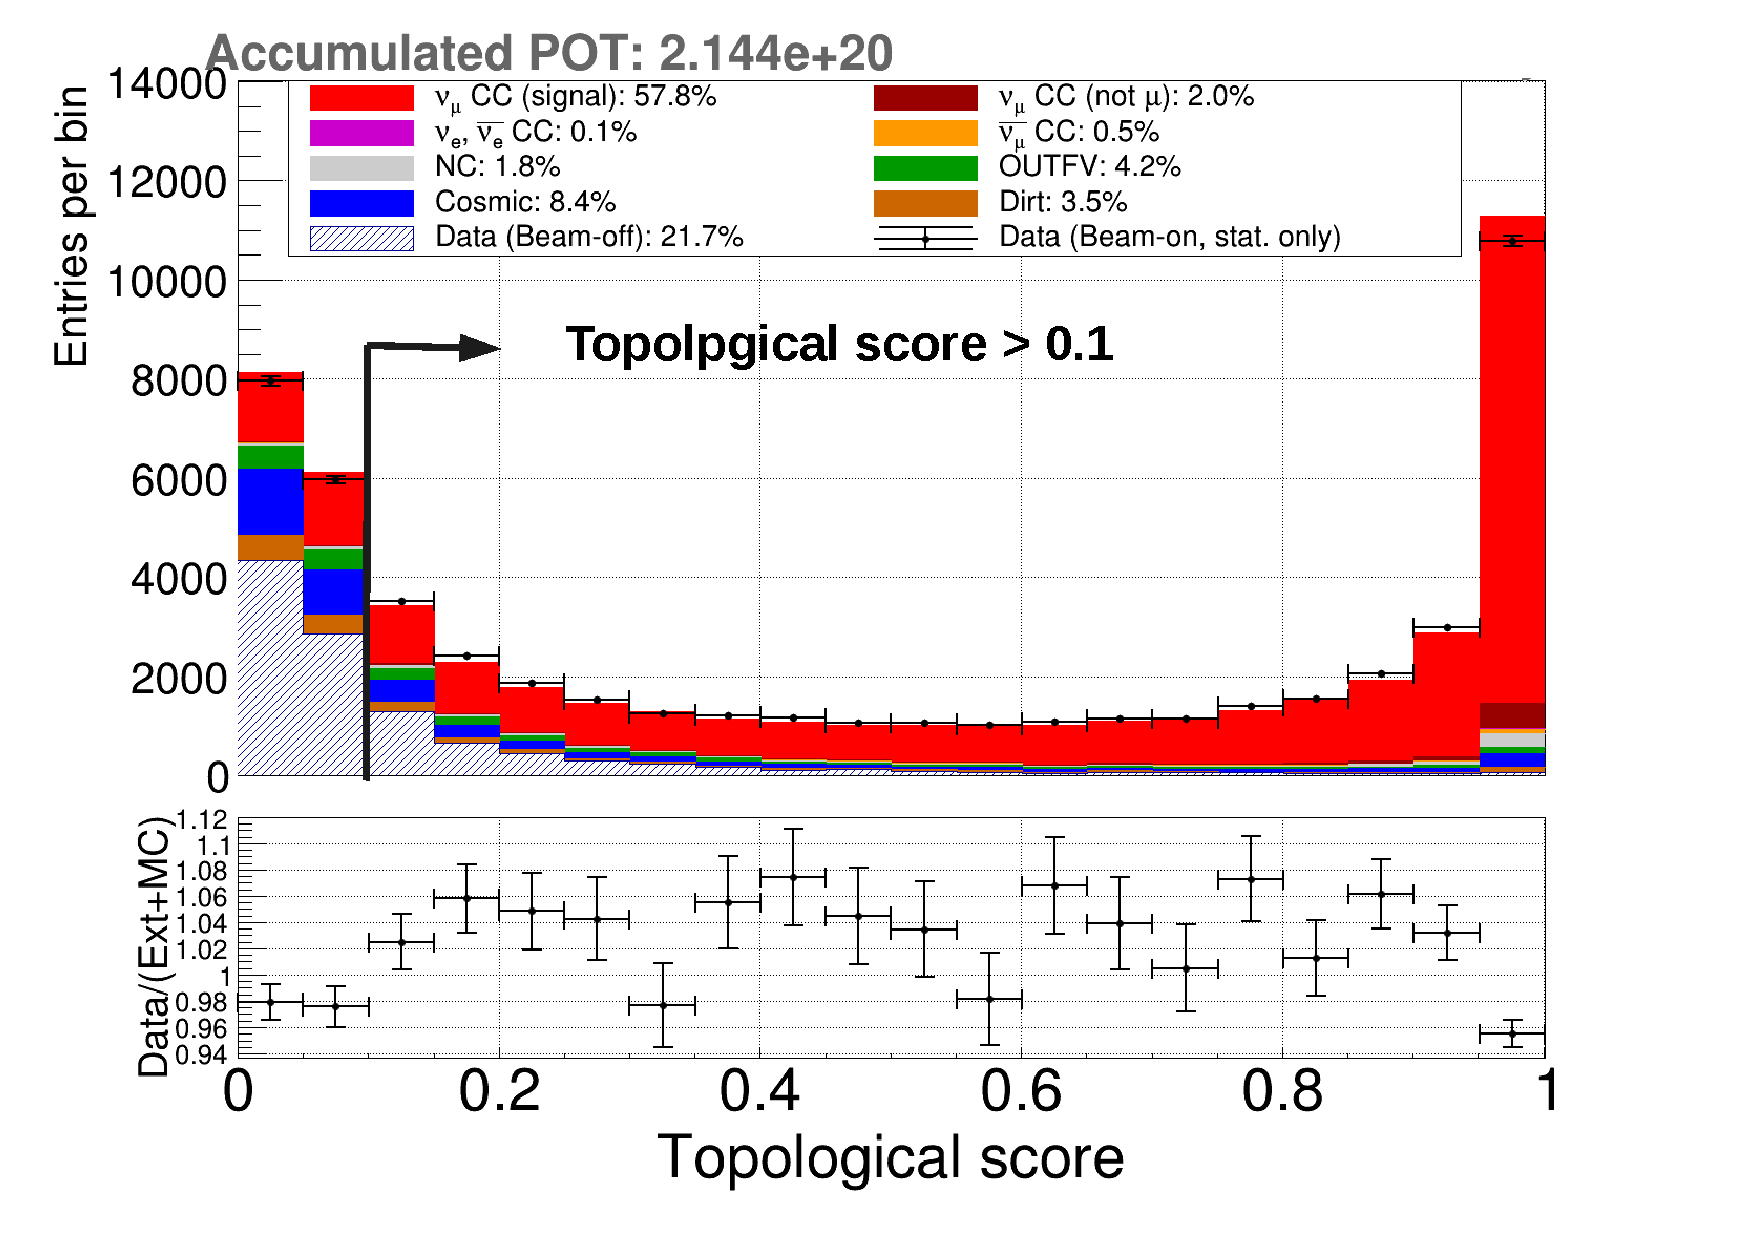
\includegraphics[width=0.7\textwidth]{images/NewCCInclusive/selection/Topological_score_01_8.pdf}
  \caption[Muon Candidate Topological Score Cut]{Topological scores of the neutrino candidate slices. We select events with topological scores greater than \num{0.1}.}
  \label{fig:topological_score_01_8}
\end{figure}

In order to summarise the above-described $\nu_{\mu}$ \gls{cc} inclusive selection steps, they are listed below:
\begin{enumerate}
	\item The reconstructed neutrino \glspl{Vertex} shall be in the \gls{fv} including distortions.
	\item There shall be no \gls{crt} hits on the top plane during the beam window.
	\item There shall be no \gls{crt} hits upstream to the reconstructed neutrino \glspl{Vertex} along the \gls{bnb} direction during the beam window.
	\item There shall be no \gls{crt} hits associated to the neutrino slice if the muon candidates are contained.
	\item The muon candidates shall not be associated to \gls{crt} hits outside of the beam window.
	\item Track scores of the muon candidates shall be greater than \num{0.8}.
	\item Track lengths of the muon candidates shall be longer than \SI{20}{\cm}.
	\item Track \gls{pid} $\chi^2$ scores for proton hypothesis of the muon candidates shall be greater than \num{78}.
	\item Topological scores of the neutrino slices shall be greater than \num{0.1}.
\end{enumerate}

% --------------------------------------------------------------------------------------------------------------------------------------------------------------------------------------------

\section{Selection Results}
All results presented here are fully forward-folded event rates. As discussed in section \ref{sec:MeasuringCrossSection}, this method has the advantages of reducing the influence of \gls{mc} models in the results and reducing statistical uncertainty, as there is no matrix to be inverted. The first result presented, the kinematic distributions after the selection process, are shown, in order to have a compatible result to the distributions of my first analysis in \ref{sec:CrossSectionResults}. However, the ultimate goal of this analysis is to present a forward-folded double-differential $\nu_\mu$ \gls{cc} inclusive event rate in the phase space of reconstructed muon momentum and muon $\cos{(\theta)}$, \ie $\partial^2N/(\partial p_\mu \partial(\cos\theta))$, and compare this to various models.

\subsection{Kinematic Distributions} \label{new:KinematicDistributions}
The kinematic distributions after the whole selection process are shown in figures \ref{fig:muon_momentum_after_cuts} and \ref{fig:muon_costheta_after_cuts}.
\begin{figure}[htbp]
  \centering
  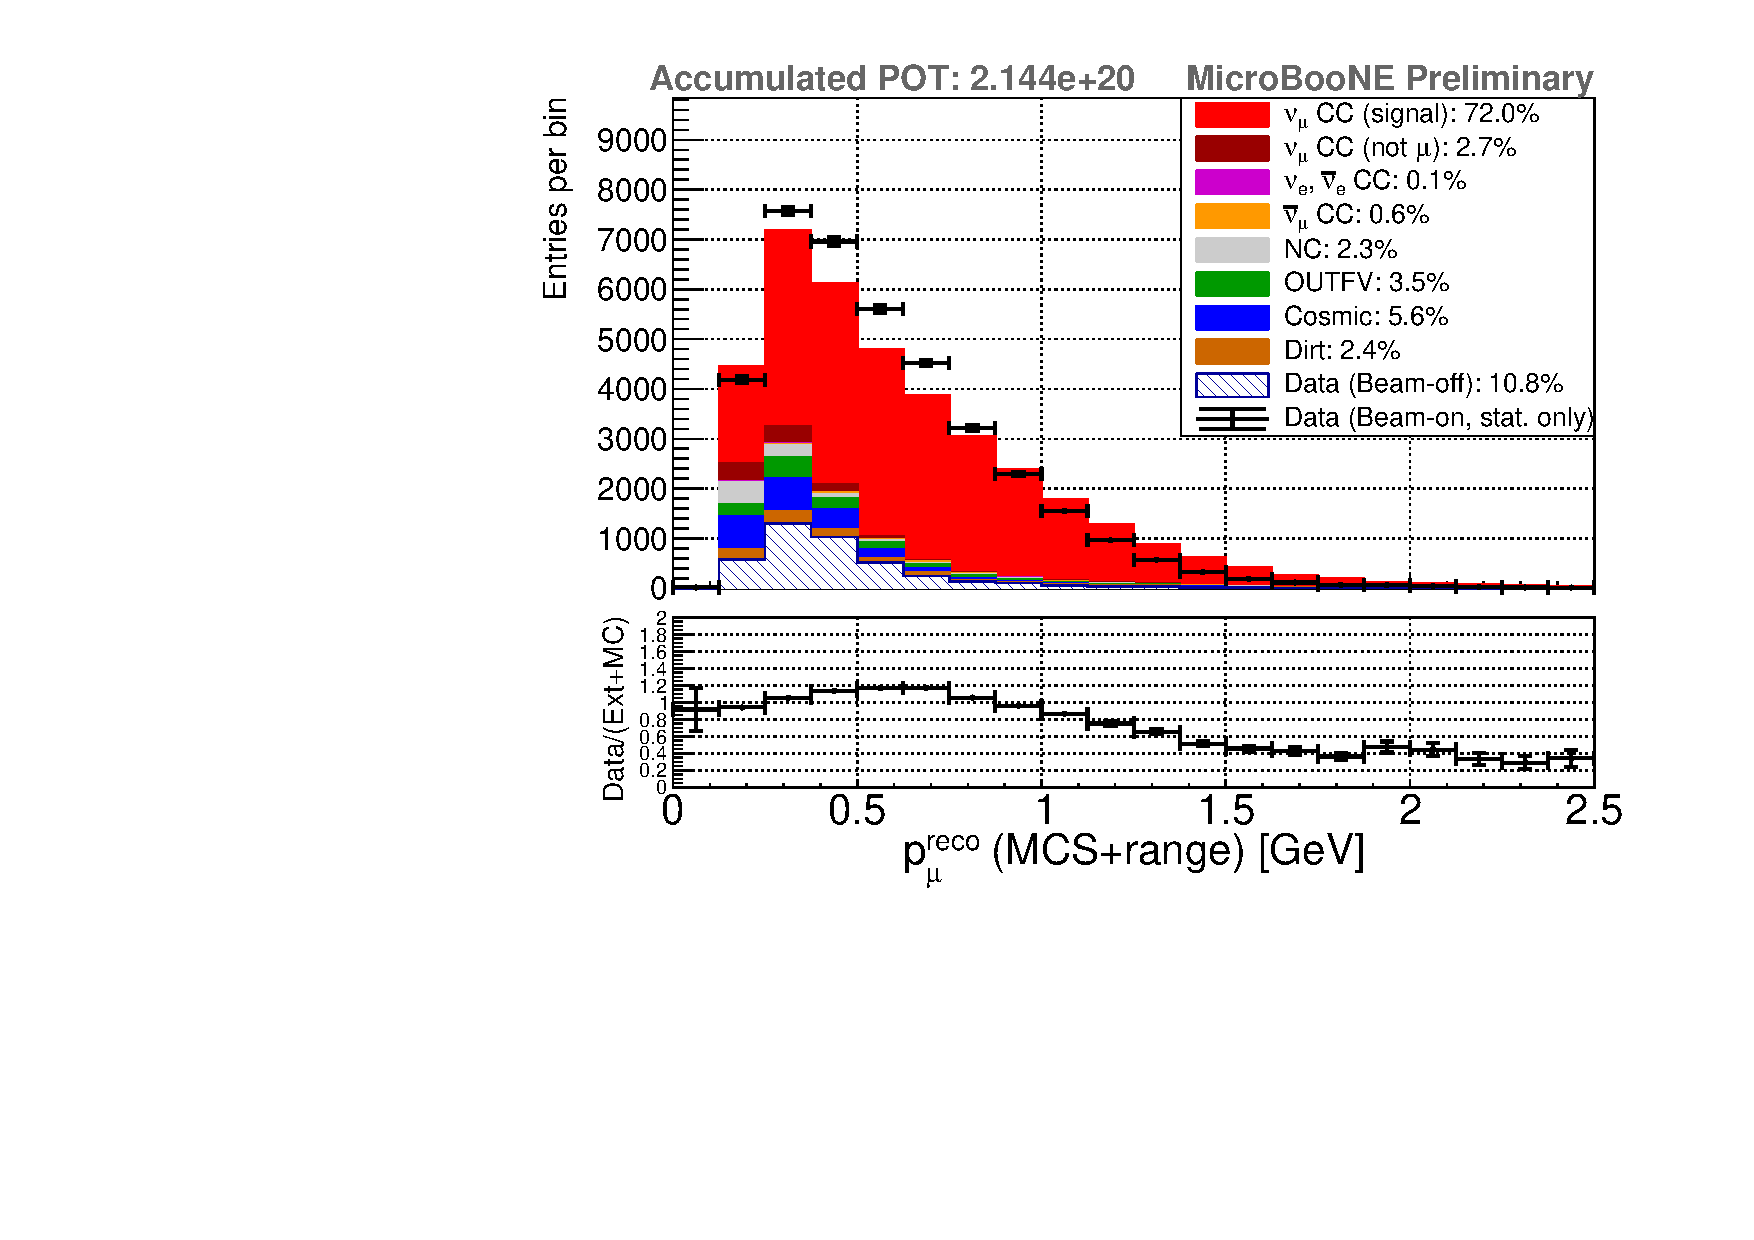
\includegraphics[width=0.7\textwidth]{images/NewCCInclusive/selection/TrackMCSRange_07.pdf}
  \caption[Forward-Folded Muon Momentum Distribution]{Reconstructed muon momentum distribution post the $\nu_\mu$ \gls{cc} inclusive selection.}
  \label{fig:muon_momentum_after_cuts}
\end{figure}
\begin{figure}[htbp]
  \centering
  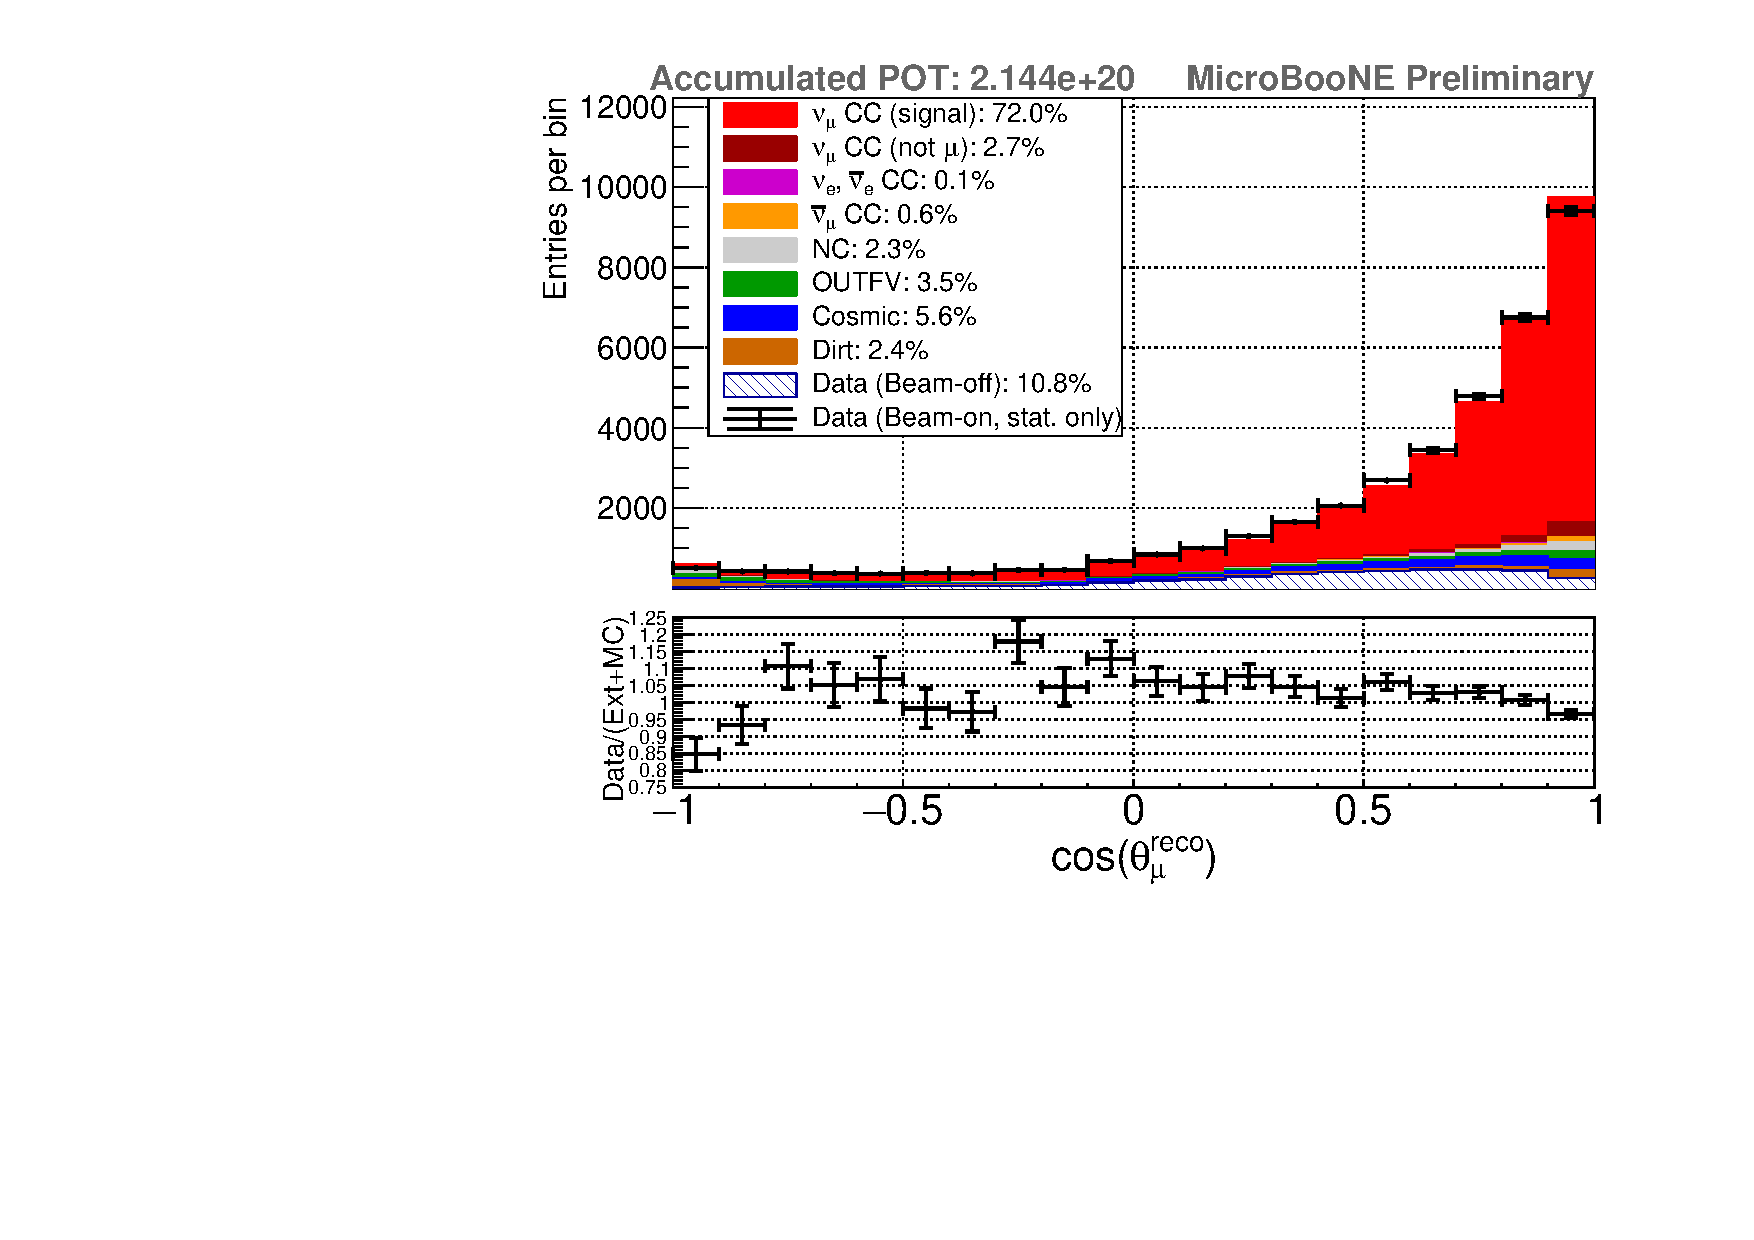
\includegraphics[width=0.7\textwidth]{images/NewCCInclusive/selection/cosTheta_07.pdf}
  \caption[Forward-Folded $\cos{(\theta)}$ Distribution]{Reconstructed muon $\cos{(\theta)}$ distribution post the $\nu_\mu$ \gls{cc} inclusive selection.}
  \label{fig:muon_costheta_after_cuts}
\end{figure}
The comparison of these graphs with the ones after the pre-selection, in figure \ref{fig:PreselectionDistributions}, shows the effectiveness of the applied cuts. Even more astonishing is the comparison between these figures and the kinematic distributions resulting from my first analysis in figures \ref{fig:ForwardFoldedCosTheta} and \ref{fig:ForwardFoldedMomentum}. The backgrounds, especially the cosmic-ray related ones, are highly reduced in the new results. This is a strong indicator for MicroBooNE's progress in the past couple of years. After the pre-selection process, the purity of the sample was \SI{33}{\percent}, and the efficiency was at \SI{69}{\percent}. Now, after the full selection, the signal purity reaches \SI{72}{\percent} and the selection efficiency \SI{56}{\percent}. All the neutrino induced backgrounds are well below \SI{5}{\percent}, hence, no dedicated control samples are selected to constrain these backgrounds.
% TODO add purity/efficiency graph here. check first cut?
% \section{Double-Differential $\nu_\mu$ CC Inclusive Cross Section}

\subsection{Double-Differential Binning} \label{sec:DoubleDifferentialBinning}
For the double-differential distributions, our analysis adopts the same binning as MicroBooNE's first double-differential $\nu_\mu$ \gls{cc} inclusive cross section in the phase space of reconstructed muon momentum and muon $\cos{(\theta)}$ \cite{MicroBooNEFirstCCInclPublished}. Said phase space is divided up into \num{42} bins within the muon momentum range from \SIrange{0}{2.5}{\GeV/c}, and the muon $\cos(\theta)$ range from \num{-1} to \num{1}, without gaps between bins. The chosen binning partition is shown in figure \ref{fig:Binning_reco_ev_rate}.
\begin{figure}[htbp]
  \centering
  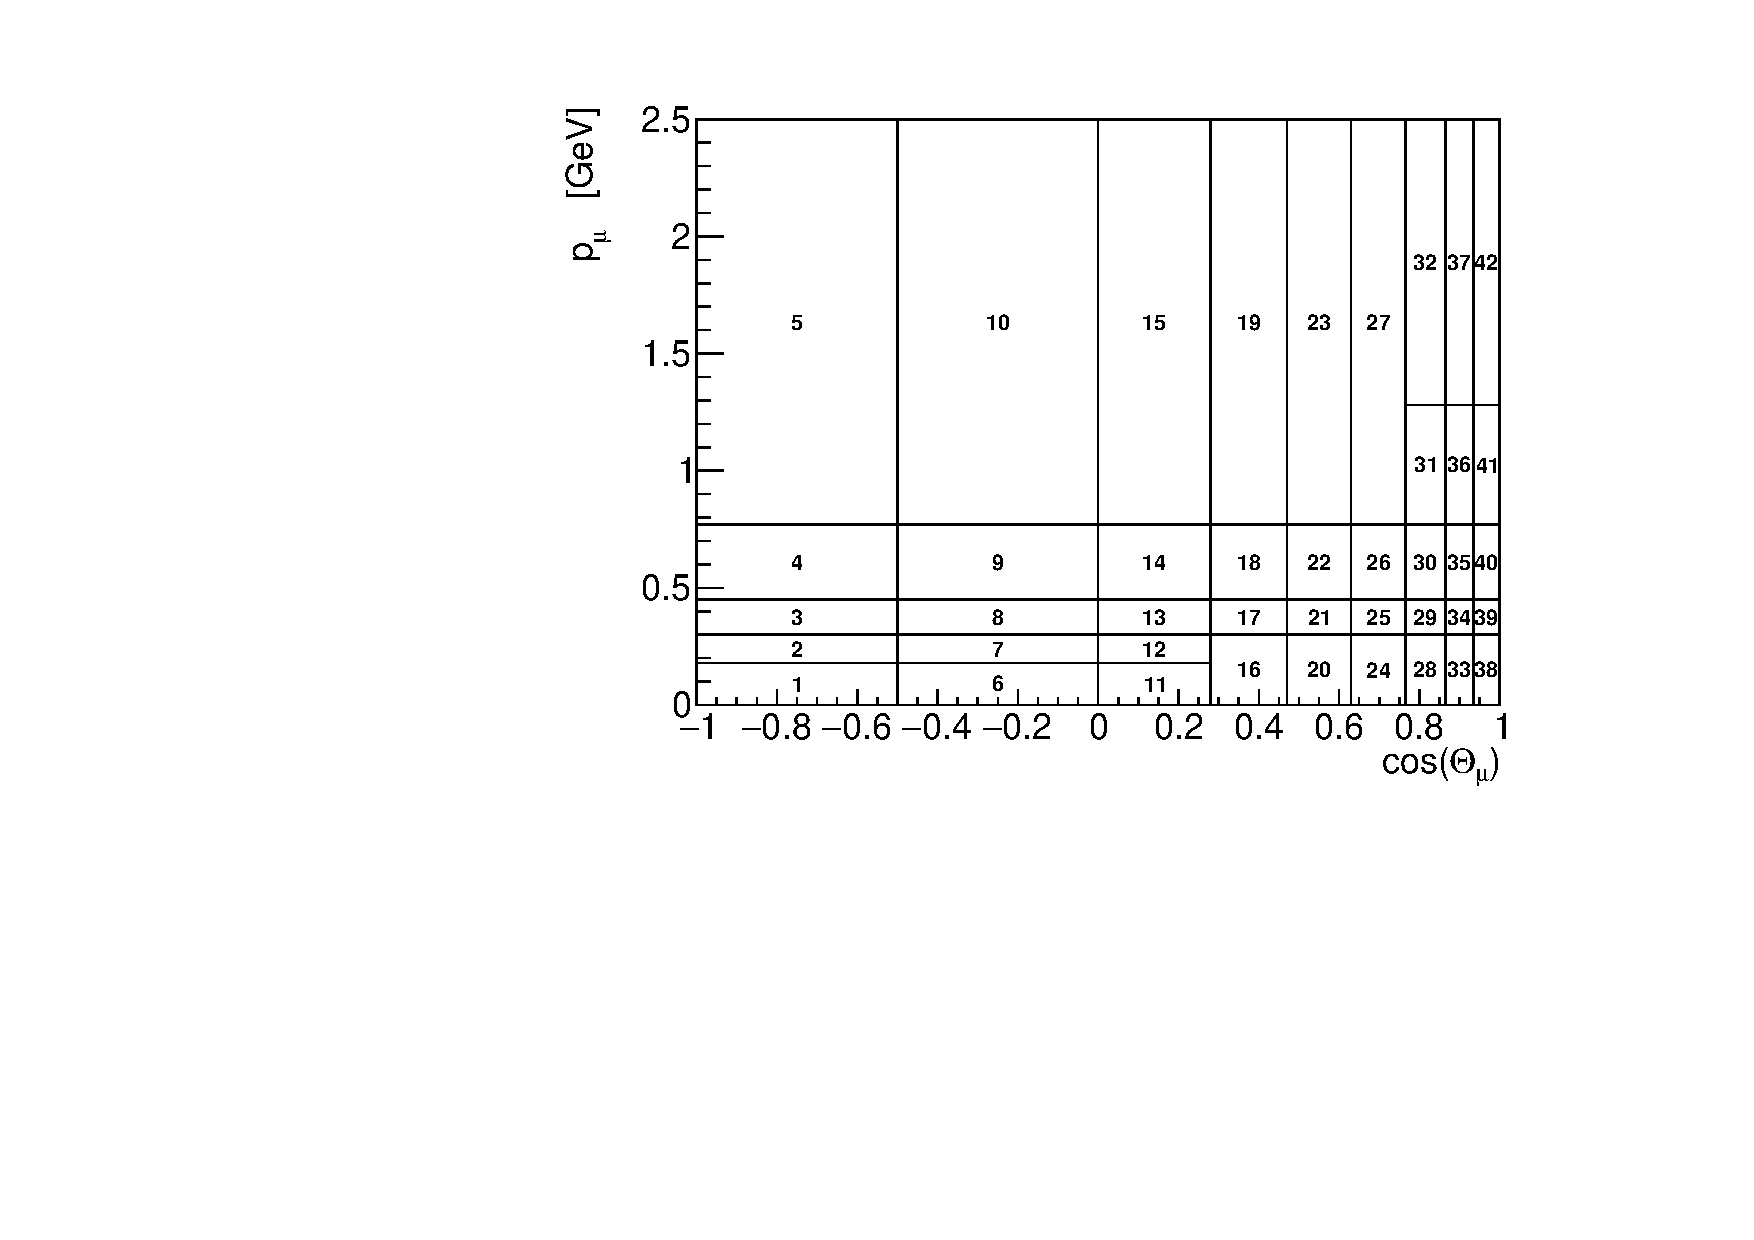
\includegraphics[width=0.7\textwidth]{images/NewCCInclusive/xsec/h_2D_binning.pdf}
  \caption[2D Binning of the Double-Differential Rate]{Shown here is the \gls{2d} binning for the double-differential rate in the phase space of $p_\mu$ and $\cos{(\theta)}$}
  \label{fig:BinningDoubleDiff}
\end{figure}
As shown in the figure, every bin gets an ID number ranging from \num{1} to \num{42}. This is used to reduce the \gls{2d} graph of the double-differential rate into a \gls{1d} histogram with said ID on the $x$-axis. This also simplifies the smearing matrix. The binning partition, is derived from the bin sizes of the single differential distributions in momentum and $\cos{(\theta)}$, merging bins with low statistics. As we will use a covariance matrix to summarise the uncertainties, the bin contents distribution should be close to a Gaussian function. Moreover, an ideal binning leads to the diagonal terms of the smearing matrix to amount to \num{0.68}.

When we fill the muon candidate properties of the selected events into the appropriate bins, the Gaussian bin contents distribution seems to be fulfilled. This is indicated by figure \ref{fig:Binning_reco_ev_rate} showing a distribution of the selected events across the reconstructed bins. In addition, we can use the same binning in true space and fill them with the selection efficiency as presented in figure \ref{fig:Binning_true_eff}.
\begin{figure}[htbp]
	\begin{center} \centering
		\subfloat[Rate]
        {
            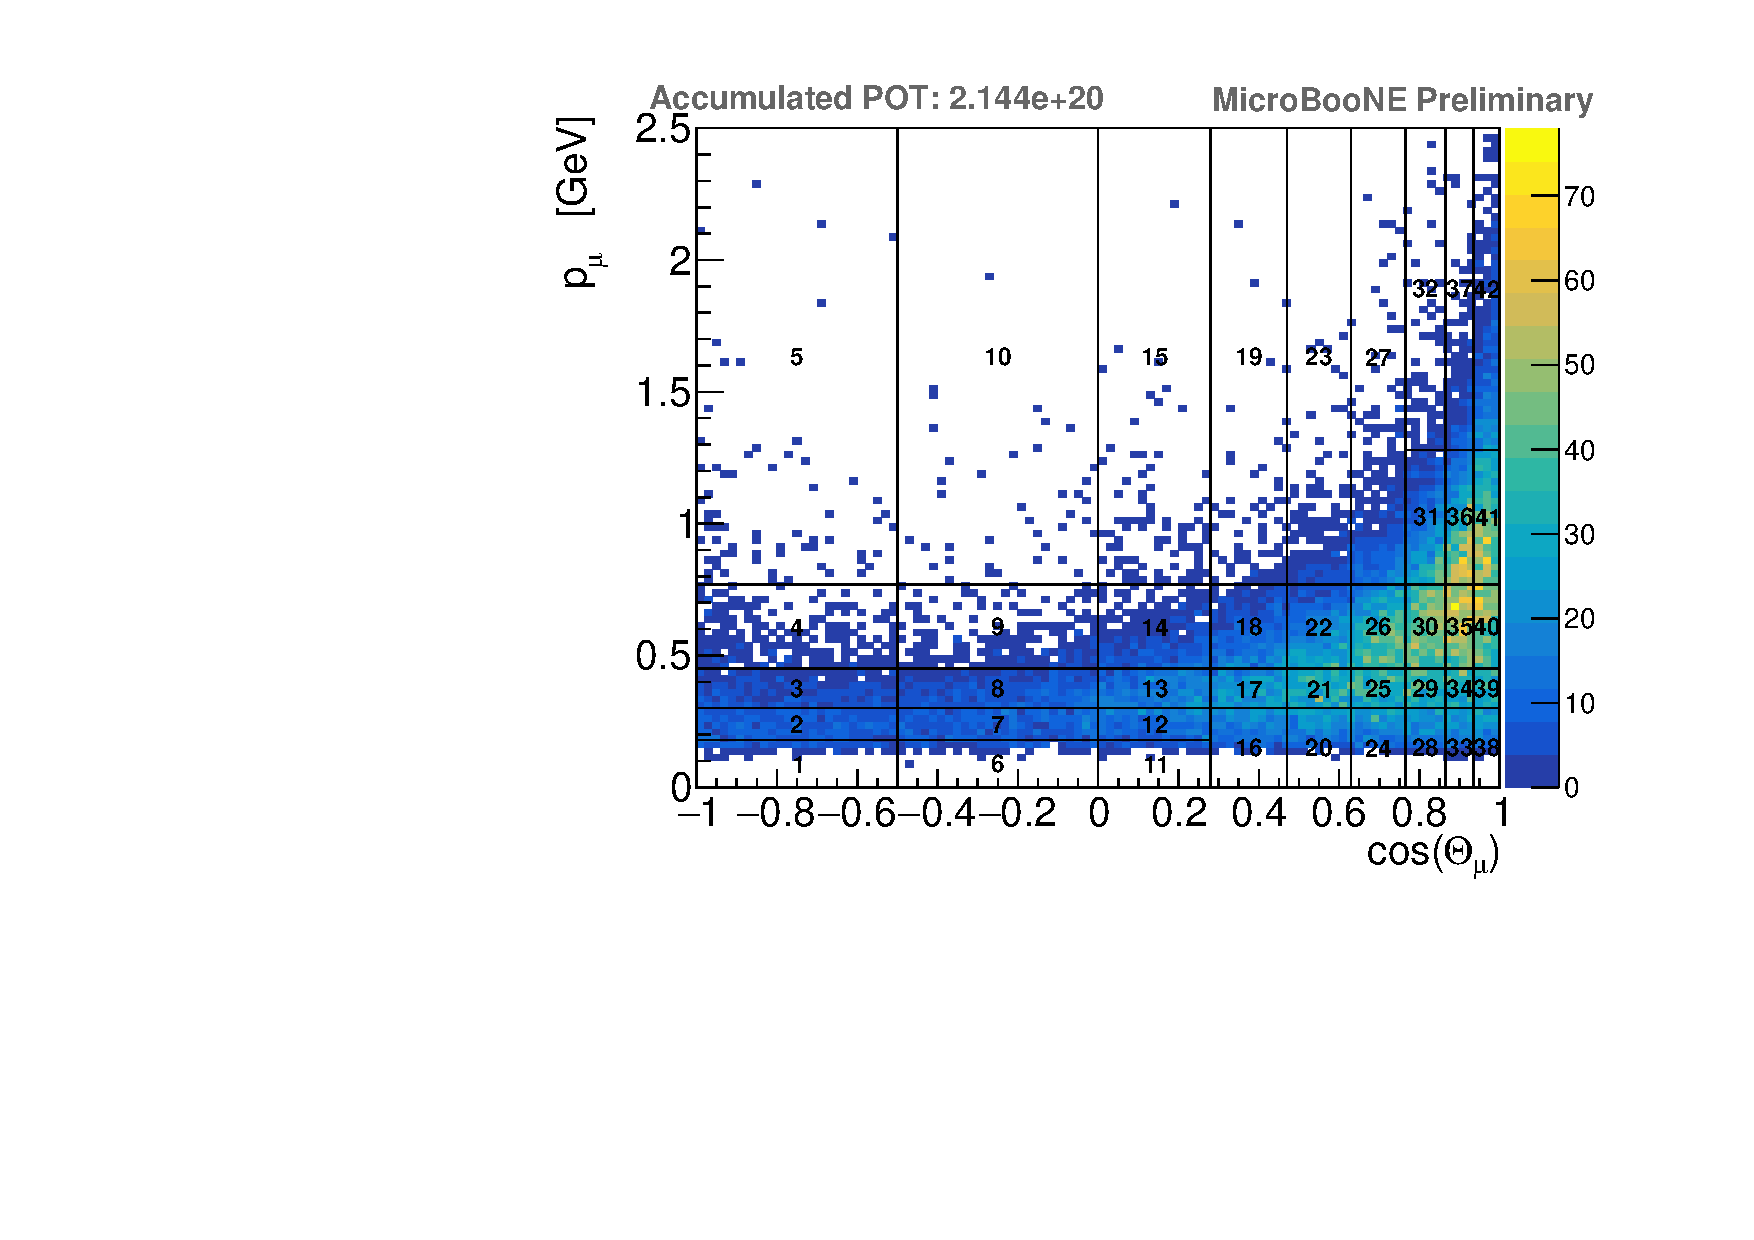
\includegraphics[width=0.49\textwidth]{images/NewCCInclusive/xsec/Binning_reco_evrate.pdf}
            \label{fig:Binning_reco_ev_rate}
        }
		\subfloat[Efficiency]
        {
            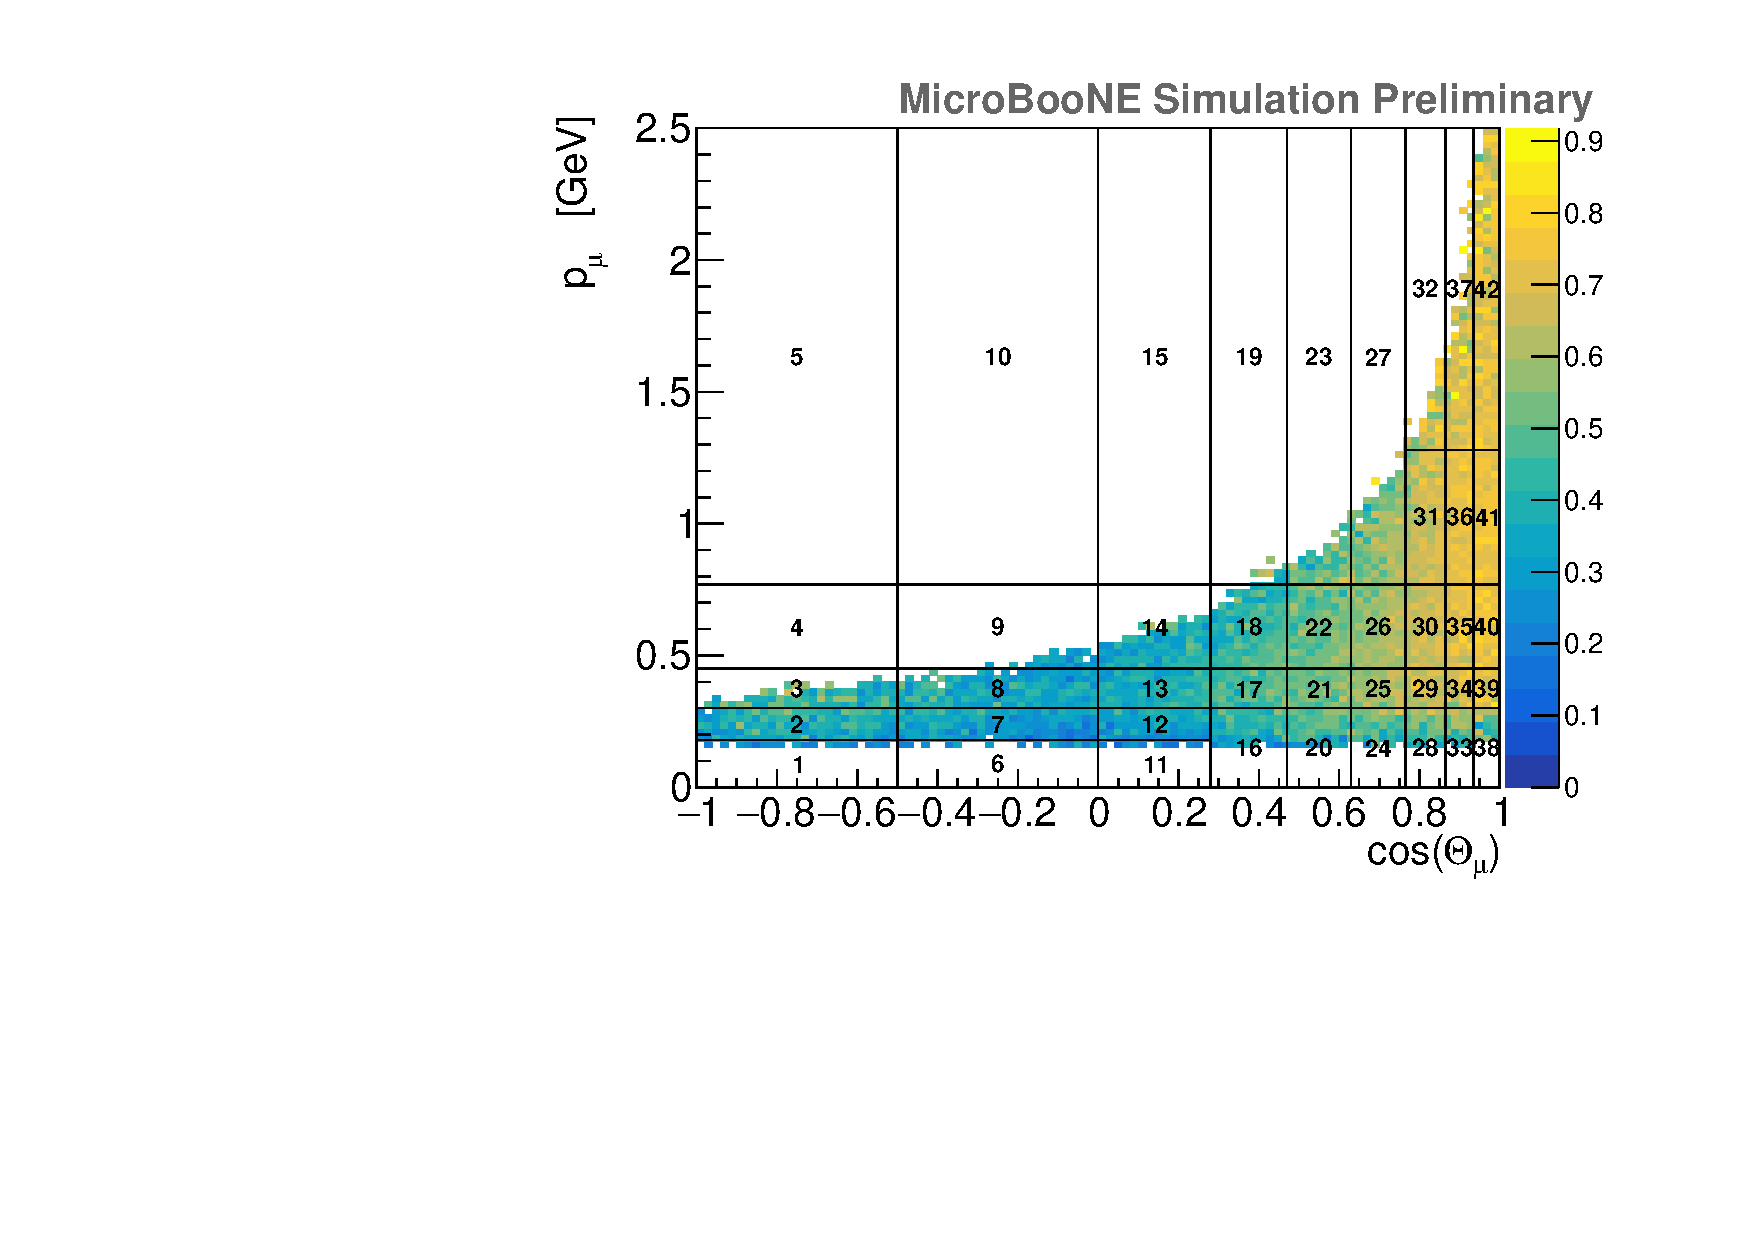
\includegraphics[width=0.49\textwidth]{images/NewCCInclusive/xsec/Binning_true_eff.pdf}
            \label{fig:Binning_true_eff}
        } 
        \caption[Filling the Double Differential Histogram]{Shown in a \subref{fig:Binning_reco_ev_rate} is the distribution of events within the double-differential bins, while \subref{fig:Binning_true_eff} depicts the double-differential selection efficiency distribution.} 
        \label{fig:FillingDoubleDiff}
	\end{center}
\end{figure}
As can be seen, there are no true backward pointing high momentum events. In reconstruction space, however, there are a few. This difference between the two graphs stems from detector smearing.
 
\subsection{Double-Differential Distribution and Model Comparison} \label{sec:DoubleDifferentialResults}
With the binning choice settled, we can now show the measured event rate with respect to the reconstructed bin ID as shown in figure \ref{fig:EventRate_data}.
\begin{figure}[htbp]
  \centering
  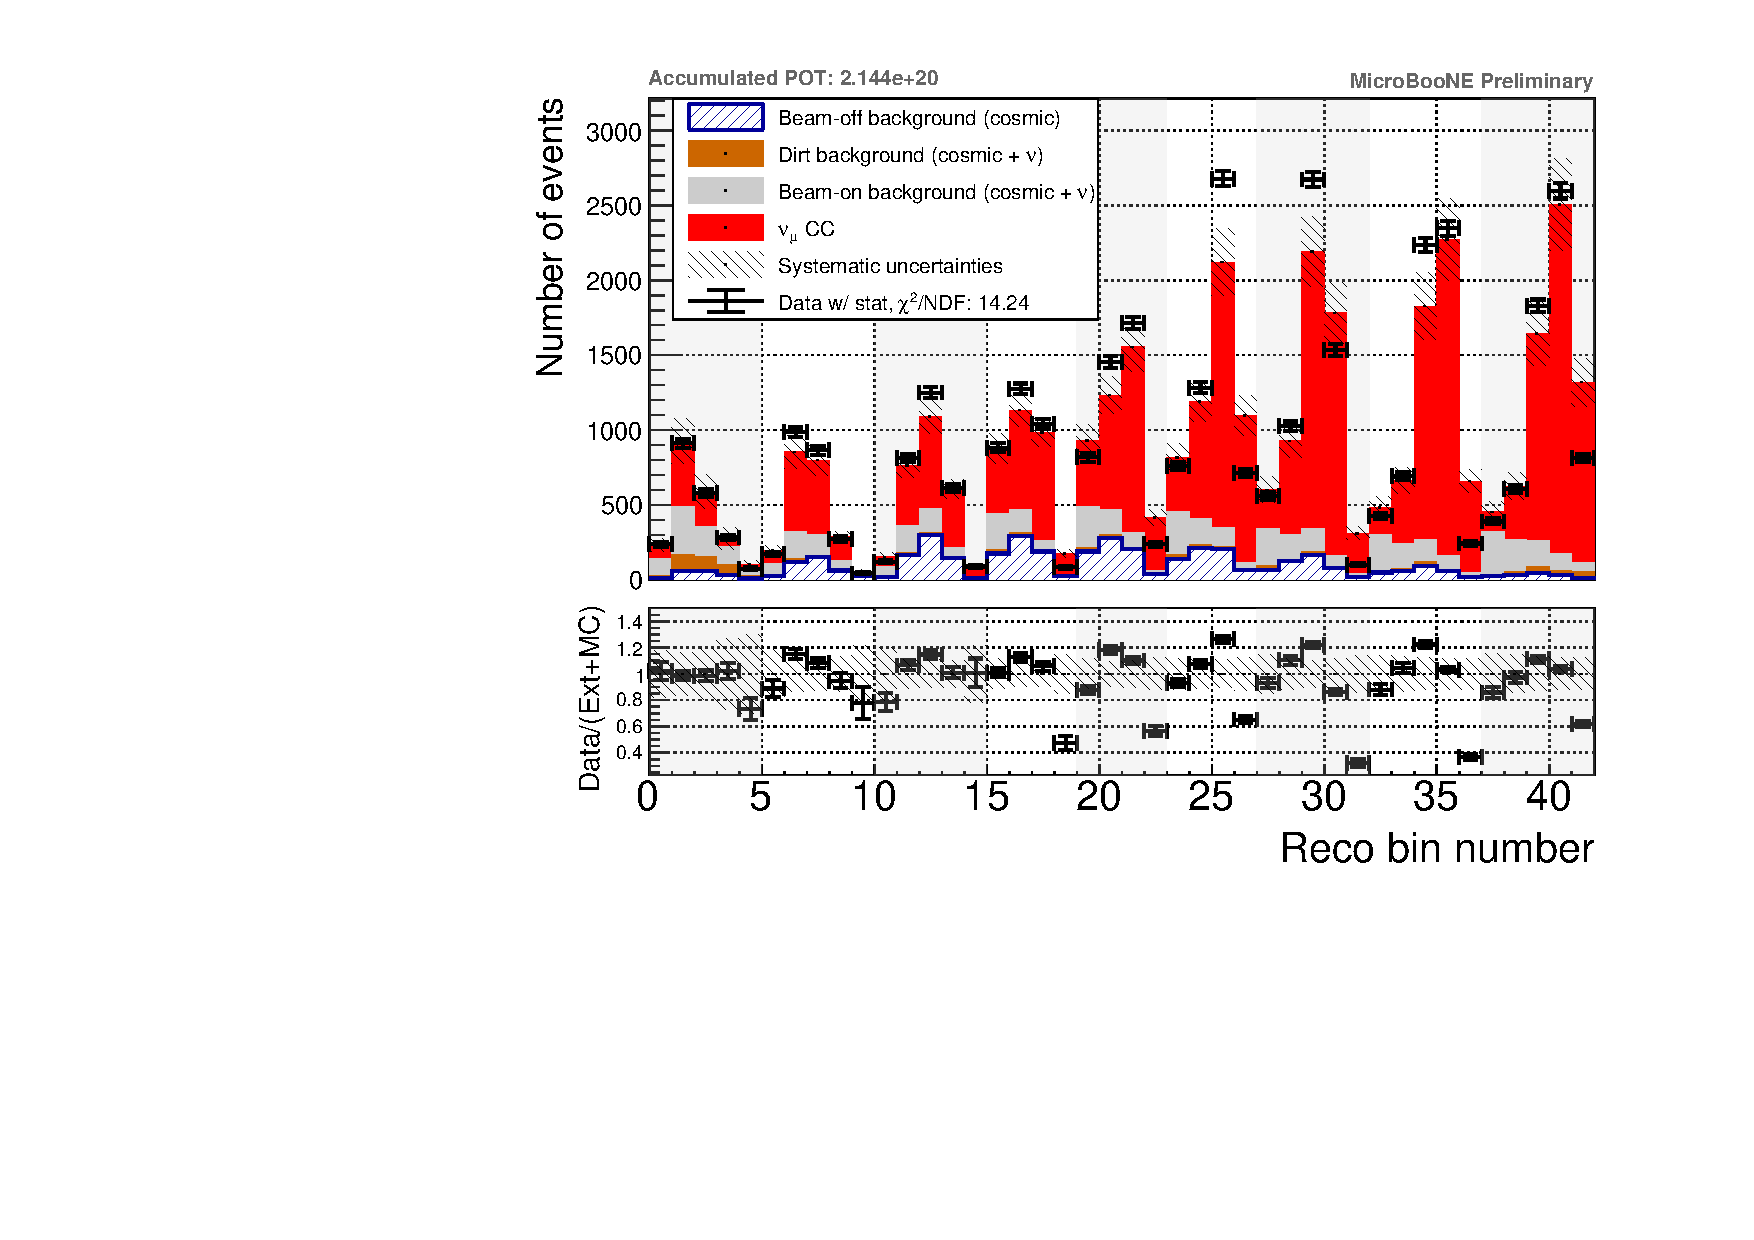
\includegraphics[width=\textwidth]{images/NewCCInclusive/xsec/EventRate_GENIEv3_tune.pdf}
  \caption[Measured Double Differential Event Rate]{The top panel shows the measured number of events per reconstructed bin with the statistical uncertainty. The modeled events with the tuned \gls{genie} v3 (the baseline simulation) are also shown as a comparison.The red histogram is the modeled $\nu_\mu$ CC signal. The gray, brown and dashed blue histograms are the backgrounds from the overlay, dirt and beam off sample respectively. The dashed gray blocks are the systematic uncertainties on each bin. The bottom panel shows the ratio between data and model with respect to the reconstructed bins.}
  \label{fig:EventRate_data}
\end{figure}
The error bars on the data points are the statistical uncertainties of the selected beam on sample. In this graph, we also plotted the modelled event rates with the tuned \gls{genie} v3 (the baseline model). The red histogram represents the modelled $\nu_\mu$ \gls{cc} signal. Also noteworthy, is the background categorisation. We now separate them by their (\gls{mc}) data sample origin rather than interaction channel. In gray we have the beam on overlay related background which includes the cosmic pileup, out of \gls{fv}, and the misidentified neutrino interactions. All dirt sample background is shown in brown, which is the same as the dirt background, since there is no other background contribution from said sample. Also unchanged, is the beam off cosmic-ray sample background represented by the dashed blue histograms. Note that the dashed dark grey blocks, overlapping the red signal histogram, show the total uncertainties on each bin, which correspond to the square root of the diagonal terms of the total covariance matrix, which we will discuss later. At the bottom of the figure, a data-to-model ratio graph is also shown including systematic (dashed area), and statistic errors (error bars). From the graph we learn, that the baseline model is not a good representation of $\nu_\mu$ \gls{cc} inclusive interactions on argon, since we find many great deviations from the data points (see bottom panel of figure \ref{fig:EventRate_data}). Consequently the $\chi^2/\text{NDF}$ value is too high with \num{14.24}, for a perfect prediction would feature $\chi^2/\text{NDF} = 1$. The $\chi^2$ is calculated using the following formula:
\begin{equation}
    \chi^2 = \sum_{ij} \left[ N^{\textrm{data}}_i - N^{\textrm{pred}}_i \right] \cdot \left[ E^{\textrm{tot}}_{ij} \right]^{-1}  \cdot \left[ N^{\textrm{data}}_j - N^{\textrm{pred}}_j \right],
\end{equation}
where $i$ and $j$ represent the bins numbers and $E^{\textrm{tot}}_{ij}$ is the total covariance matrix element of the prediction at the coordinate $ij$. The terms $N^{\textrm{data}}_i$ and $N^{\textrm{pred}}_i$ stands for the number of events in bin $i$ measured in the beam sample and its prediction sample, respectively. The total covariance matrix will be introduced later in section \ref{sec:NewUncertainties} and is defined in equation \ref{eq:sum_cov}. The number of degrees of freedom, \ie $\text{NDF}$, is given by the number of bins and is thus \num{42}, as so many answers about the universe.

% TODO reformating? glossaries? explain models, like thomas did?
Using the forward-folding methode described in section \ref{sec:MeasuringCrossSection} we used five more models for comparison with our selected data. These generators are:
\begin{itemize}
	\item \gls{genie} v3.00.04 (version 3)
	\item \gls{genie} v2.12.10 (version 2)
	\item NEUT version 5.4.0.1
	\item NuWro version 19.02.1
	\item GiBUU release 2019
\end{itemize}
The $\chi^2/\text{NDF}$ values for all the model comparisons to our selection sample are listed in table \ref{tab:chi2_comp}. Also, here the models are a bad representation of the measured reality. With $\chi^2/\text{NDF}$ between \num{12.34} and \num{15.47} there are only minor quality differences between these generators. It is also striking, that the sources of these high $\chi^2/\text{NDF}$ values are always same bins (bin ID \num{19}, \num{26}, \num{27}, \num{30}, \num{32}, \num{35}, \num{37}, and \num{42}). These bins are dramatically off for almost every of these models, see figure \ref{fig:data_model}. These model discrepancies are one of the main arguments in favour of a forward-folding analysis, since this approach reduces model dependency of the measurement.
\begin{table}[h!]
	\centering
	\begin{tabular}{c|c|c|c|c|c|c}
		\toprule
		%Model & \multicolumn{2}{c}{Uncertainty} \\
		Model 			& \gls{genie} v3 tune	&	\gls{genie} v3	&	\gls{genie} v2	&	NEUT 	&	NuWro	&	GiBUU \\
%		\hline
%		total $\chi^2$	&	597.927948355	&	646.249972616	&	649.699338493	&	518.421430301	&	588.873003729	&	524.328393062\\
%		$\chi^2$/NDF	&	14.236380	&	15.386904	&	15.469032	&	12.343367	&	14.020786	&	12.484009\\
%		\hline
		
		\midrule
		total $\chi^2$	&	597.9	&	646.2	&	649.7	&	518.4	&	588.9	&	524.3\\
		$\chi^2$/NDF	&	14.24	&	15.39	&	15.47	&	12.34	&	14.02	&	12.48\\
		\bottomrule
		
	\end{tabular}
	\caption[$\chi^2$ Values for Different Neutrino Interaction Models]{Summary of the $\chi^2$ values of the data to MC comparison using different models. The uncertainties are recalculated for each model using the varied detector smearing matrices and the true distribution of the model.  The number of degrees of freedom is 42 since that many bins are used. The before discussed baseline model}
	\label{tab:chi2_comp}
\end{table}

\begin{figure}[htbp]
  \centering
  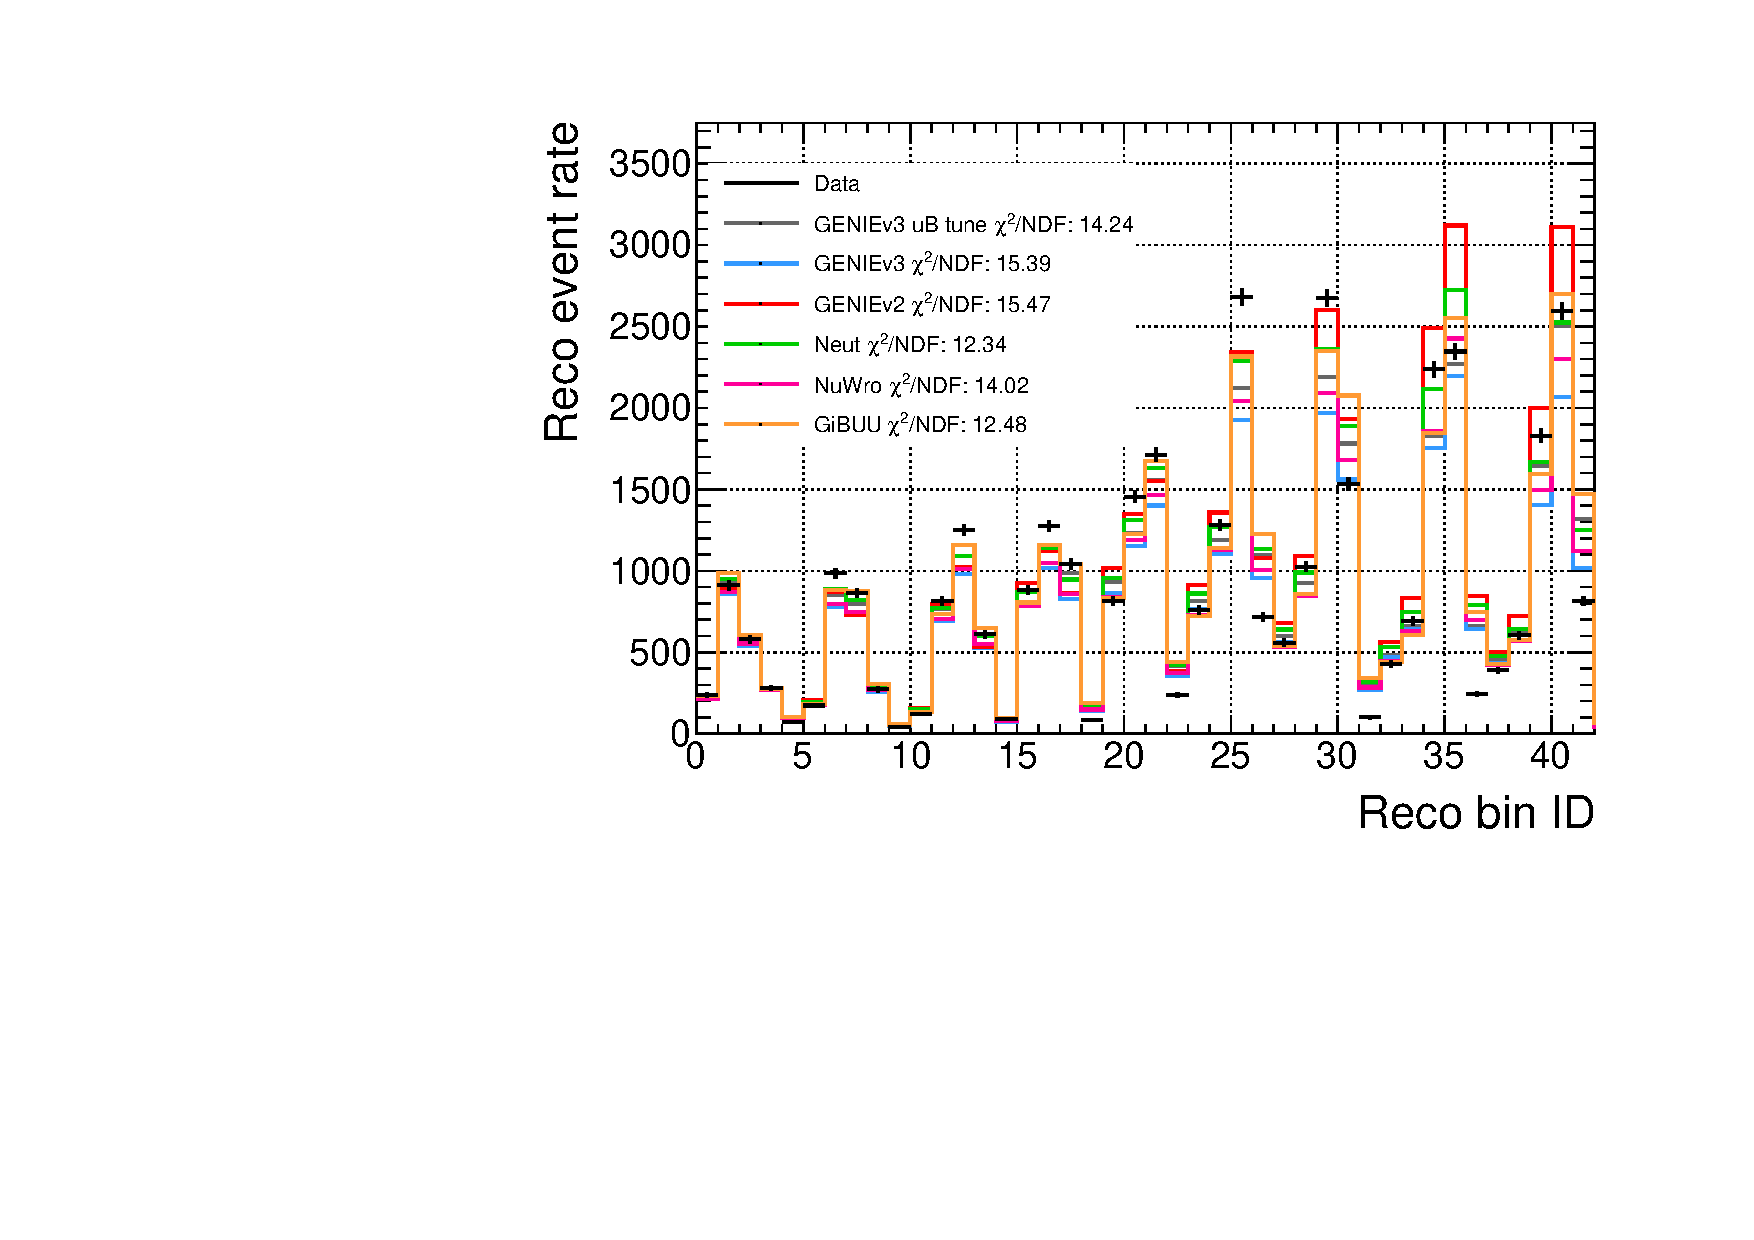
\includegraphics[width=0.7\textwidth]{images/NewCCInclusive/xsec/data_generator_comparison_chi2NDF.pdf}
  \caption[Multiple Model Comparison]{This graph shows a comparison of the double-differential $\nu_\mu$ \gls{cc} inclusive measurement (black data points), with the various models listed above depicted in differently coloured lines. It can be observed that certain bins are modelled badly by all neutrino generators.}
  \label{fig:data_model}
\end{figure}

\subsection{Smearing Matrix} \label{sec:NewDetectorSmearing}
As already mentioned in section \ref{sec:DetectorSmearing}, the smearing matrix marks the link between the true space and the reconstruction space. In this analysis we use the letter $S$ instead of $U$, but it is defined as in the theory (see equation \ref{eq:SmearingMatrix}):
\begin{equation}
    S_{ij} \coloneqq \frac{\text{\# selected reconstruction events in bin }i \text{ with a truth value in bin }j}{\text{\# generated truth events in bin }j}.
\end{equation}
In this form the smearing matrix already contains the efficiency, unlike in my first analysis. As hinted at before, the smearing matrix uses the bin ID of the double-differential distribution as its coordinates.
\begin{figure}[htbp]
  \centering
  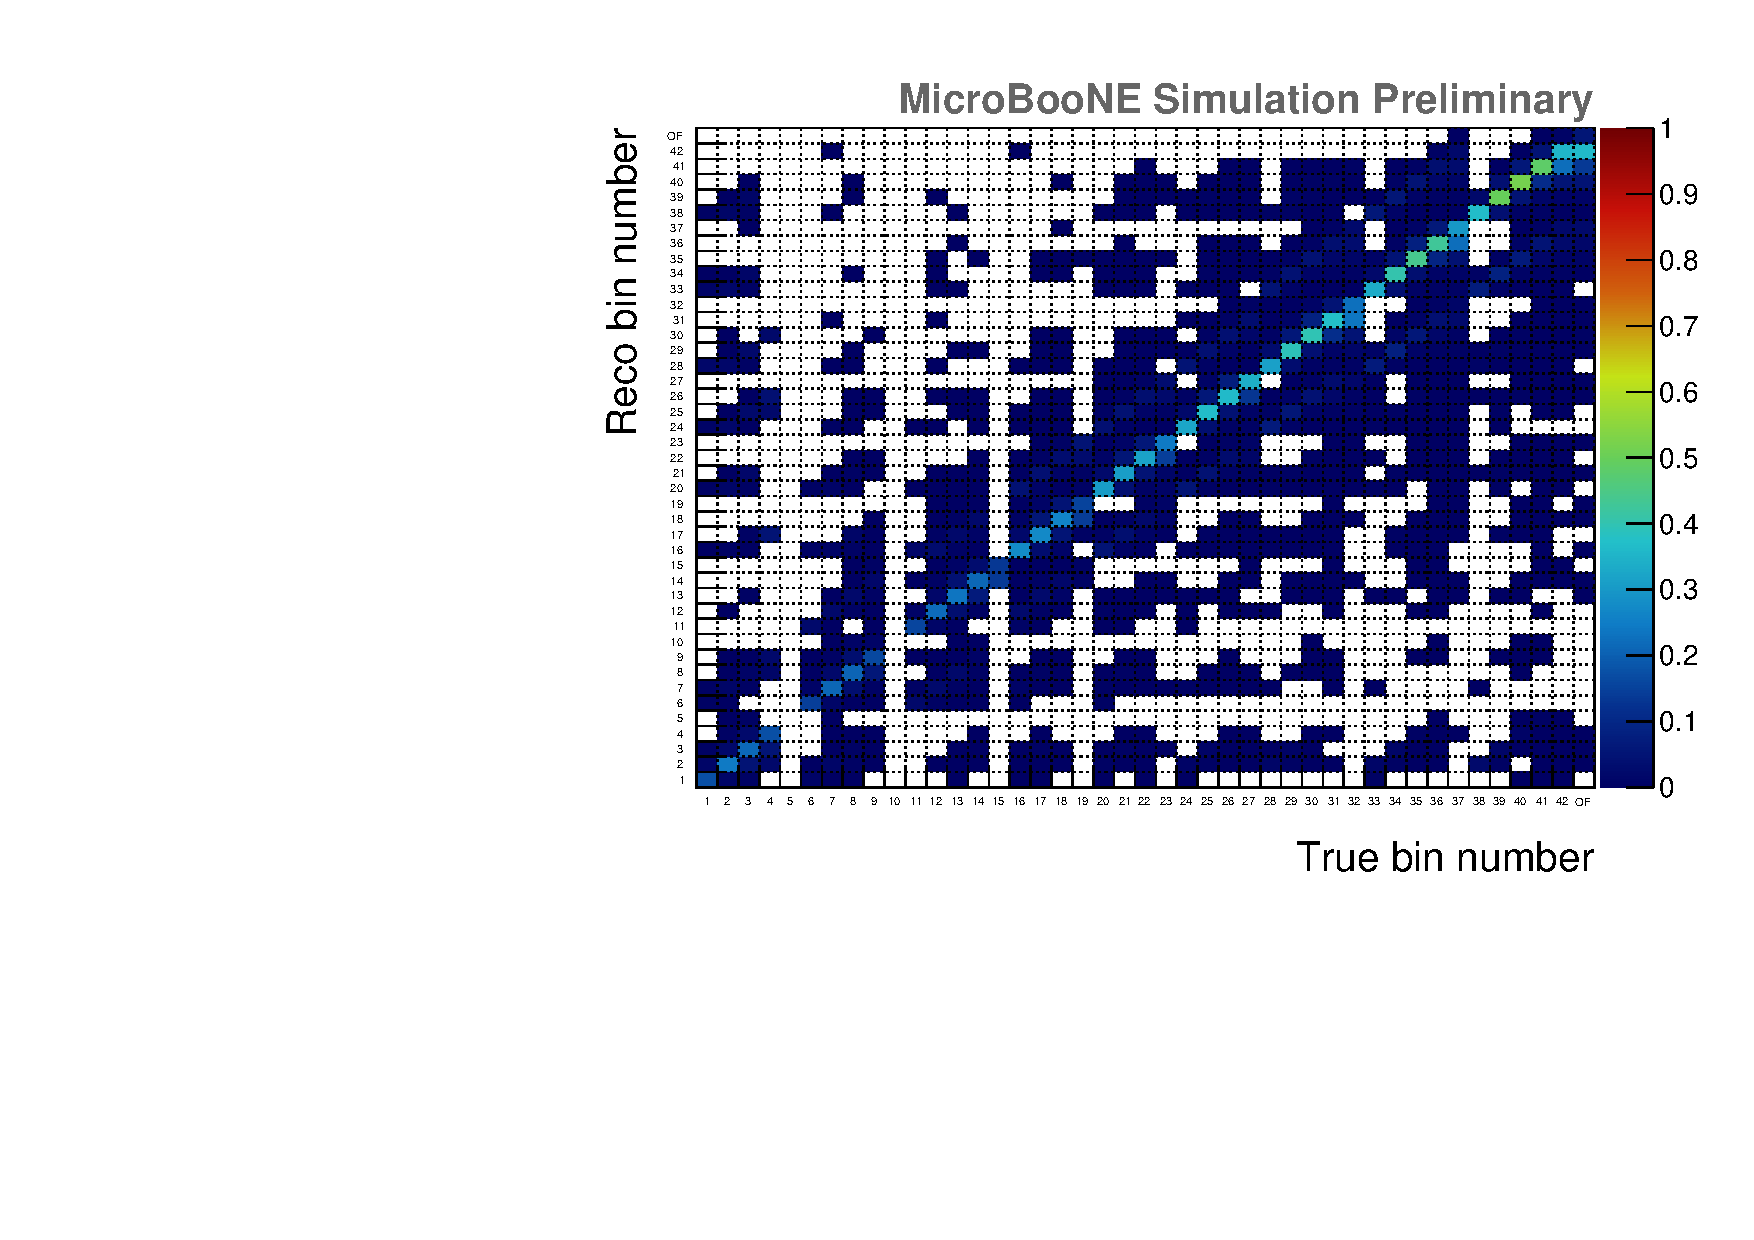
\includegraphics[width=\textwidth]{images/NewCCInclusive/xsec/Smearing_matrix_tunedGENIEv3.pdf}
  \caption[Bin ID Smearing Matrix]{The smearing matrix is produced with the default simulation. The horizontal (vertical) axis is for true (reconstructed) bins. An overflow bin is included in both phase spaces to cover muon momentum greater than \SI{2.5}{\GeV/c}. The values of the smearing matrix elements are represented by color within the range between 0 and 1.}
  \label{fig:Smearing_matrix_tunedGENIEv3}
\end{figure}
Without the included efficiency, most diagonal elements are found to be in the range of 0.6 and 0.7. This is another indicator for a sufficient bin size. 

\subsection{Uncertainties} \label{sec:NewUncertainties}
We have to consider systematic and statistical uncertainties for this forward-folded measurement of $\nu_\mu$ \gls{cc} inclusive cross section. The main sources of systematic uncertainties are detector, flux and cross-section modeling. However, we also include dirt modeling, POT counting and CRT efficiency as part of the systematic uncertainties. Both, the smearing matrix and the predicted background, are subjected to almost all systematic uncertainties, except for dirt systematics which only affects background predictions. The systematic uncertainties are evaluated through a so-called \textbf{multisim} technique \cite{SystErrorsUniverses}. Said technique is based on the generation of many \gls{mc} alternatives whereby the model parameters are varied within their respective uncertainty. Each of these varied simulations is called a \textbf{universe}. The resulting distributions of a number $M$ (in our case usually $M = 1000$) of these universes is then used to create a covariance matrix as follows,
\begin{equation}\label{eq:cov_multisim}
E_{ab} = \dfrac{1}{M} \sum^{M}_{s=0} (N^s_a - N^\text{CV}_a) \cdot (N^s_b - N^\text{CV}_b).
\end{equation}
Here, $E_{ab}$ denotes the covariance between the reconstructed bins $a$ and $b$. $N^\text{CV}_a$ ($N^\text{CV}_b$) is the central value of the predicted number of events in bin $a$ ($b$), \ie the unvaried prediction. $N^s_a$ ($N^s_b$) stands for the predicted number of events in bin $a$ ($b$) according to the universe with index $s$. Note that, every background category is varied separately and thus every category has its own covariance matrix. The total covariance matrix is simply the sum of all covariance matrices from different uncertainties:
\begin{equation} \label{eq:sum_cov}
E^\text{tot} = E^\text{flux} + E^\text{det} + E^\text{xsec} + E^\text{dirt} + E^\text{POT} + E^\text{CRT} + E^\text{stat}.
\end{equation}
In our case we have seven covariance matrices produced by the uncertainties of flux ($E^\text{flux}$), detector ($E^\text{det}$), cross section models ($E^\text{xsec}$), dirt events ($E^\text{dirt}$), \gls{pot} ($E^\text{POT}$), \gls{crt} ($E^\text{CRT}$), and finally covariance matrix of the statistical uncertainties ($E^\text{stat}$). The latter is a special case, as it only consists of the statistical variance of every bin in the diagonal of the matrix, all other entries remain zero. To calculate the error bars (dashed blocks in figure \ref{fig:EventRate_data}) of the \gls{mc} prediction, one simply takes the square root of the total variance, \ie the diagonal elements of $E^\text{tot}$. Note that, the covariance matrix provides bin-to-bin correlation information which is not shown in figure \ref{fig:EventRate_data}. Various multisim examples for different systematic uncertainties are shown in figure \ref{fig:SystematicUncertainties}.
\begin{figure}[htbp]
	\begin{center} \centering
		\subfloat[Flux]
        {
            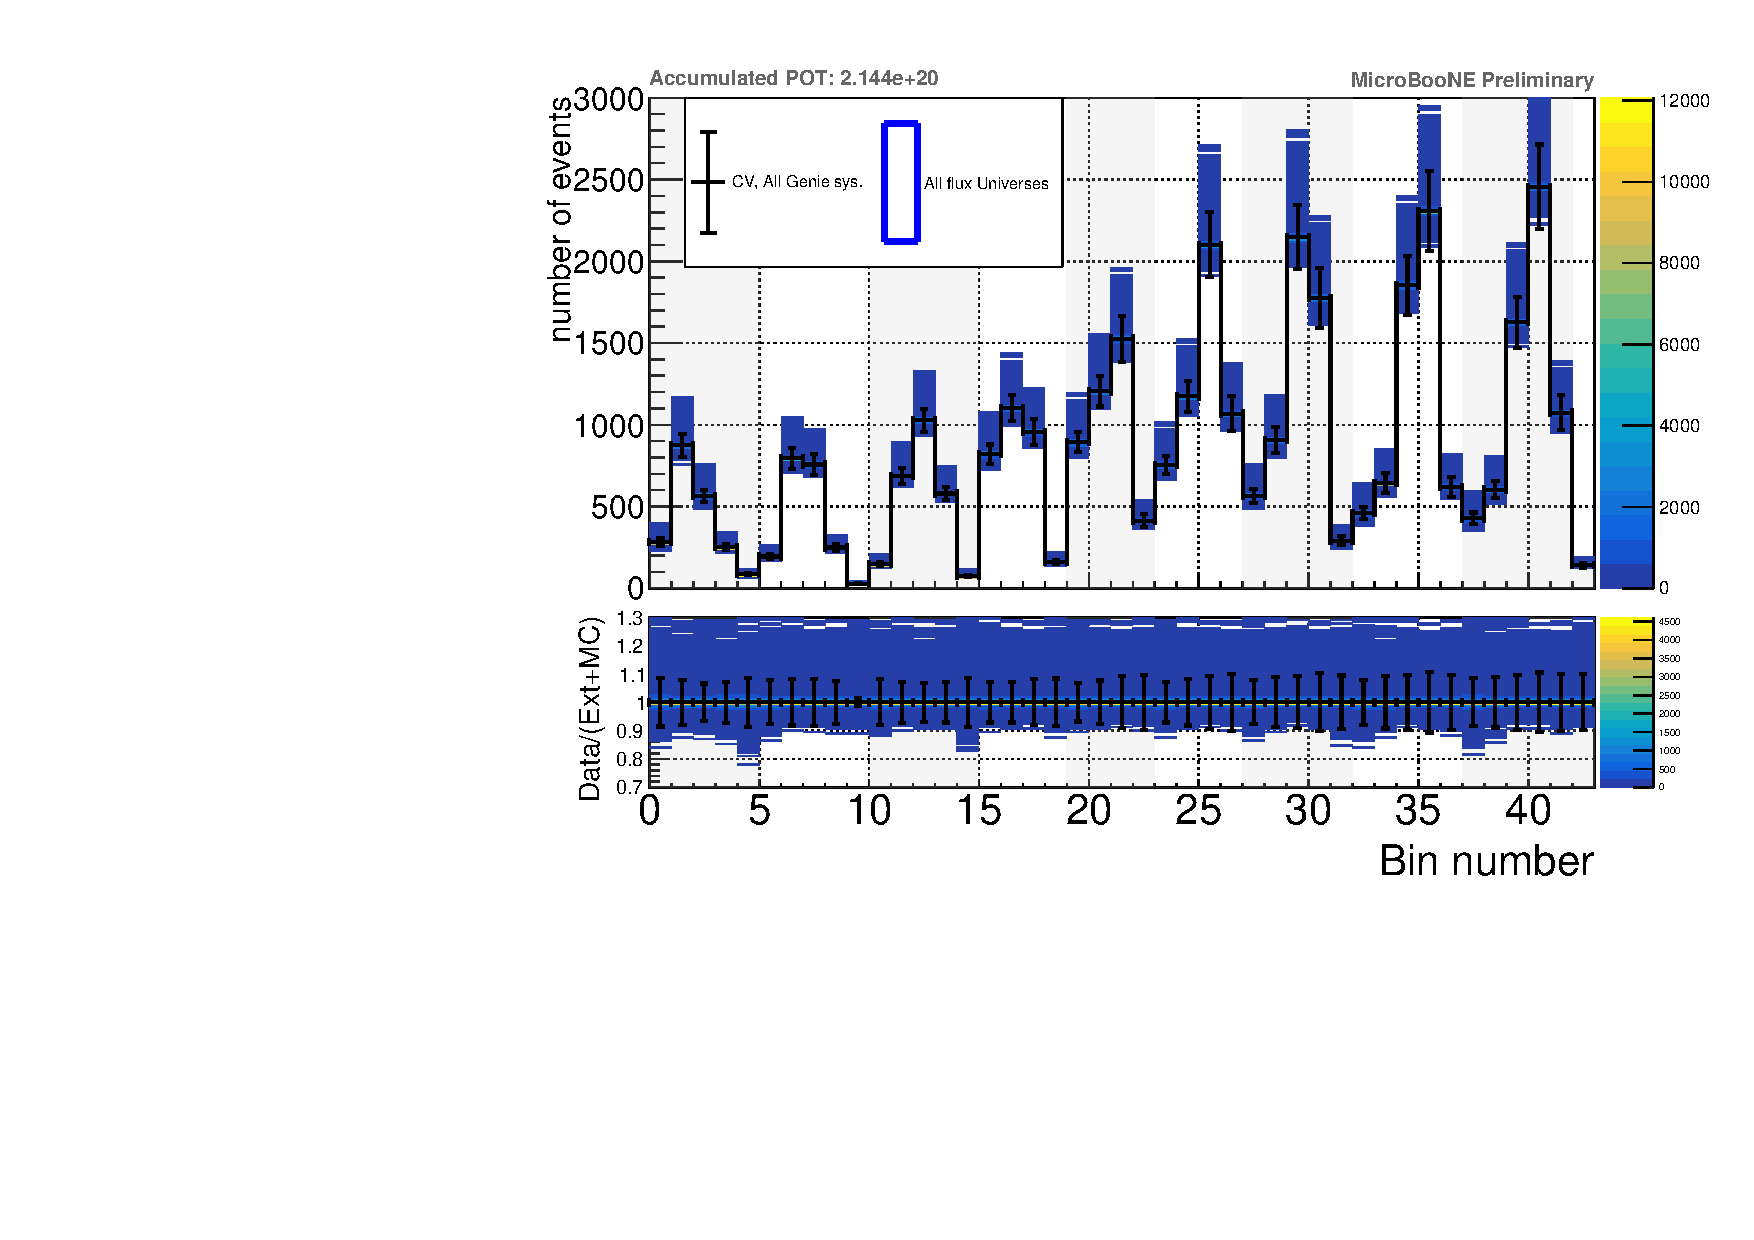
\includegraphics[width=0.49\textwidth]{images/NewCCInclusive/xsec/h_xsec_fluxsys.pdf}
            \label{fig:fluxsys}
        }
		\subfloat[Detector]
        {
            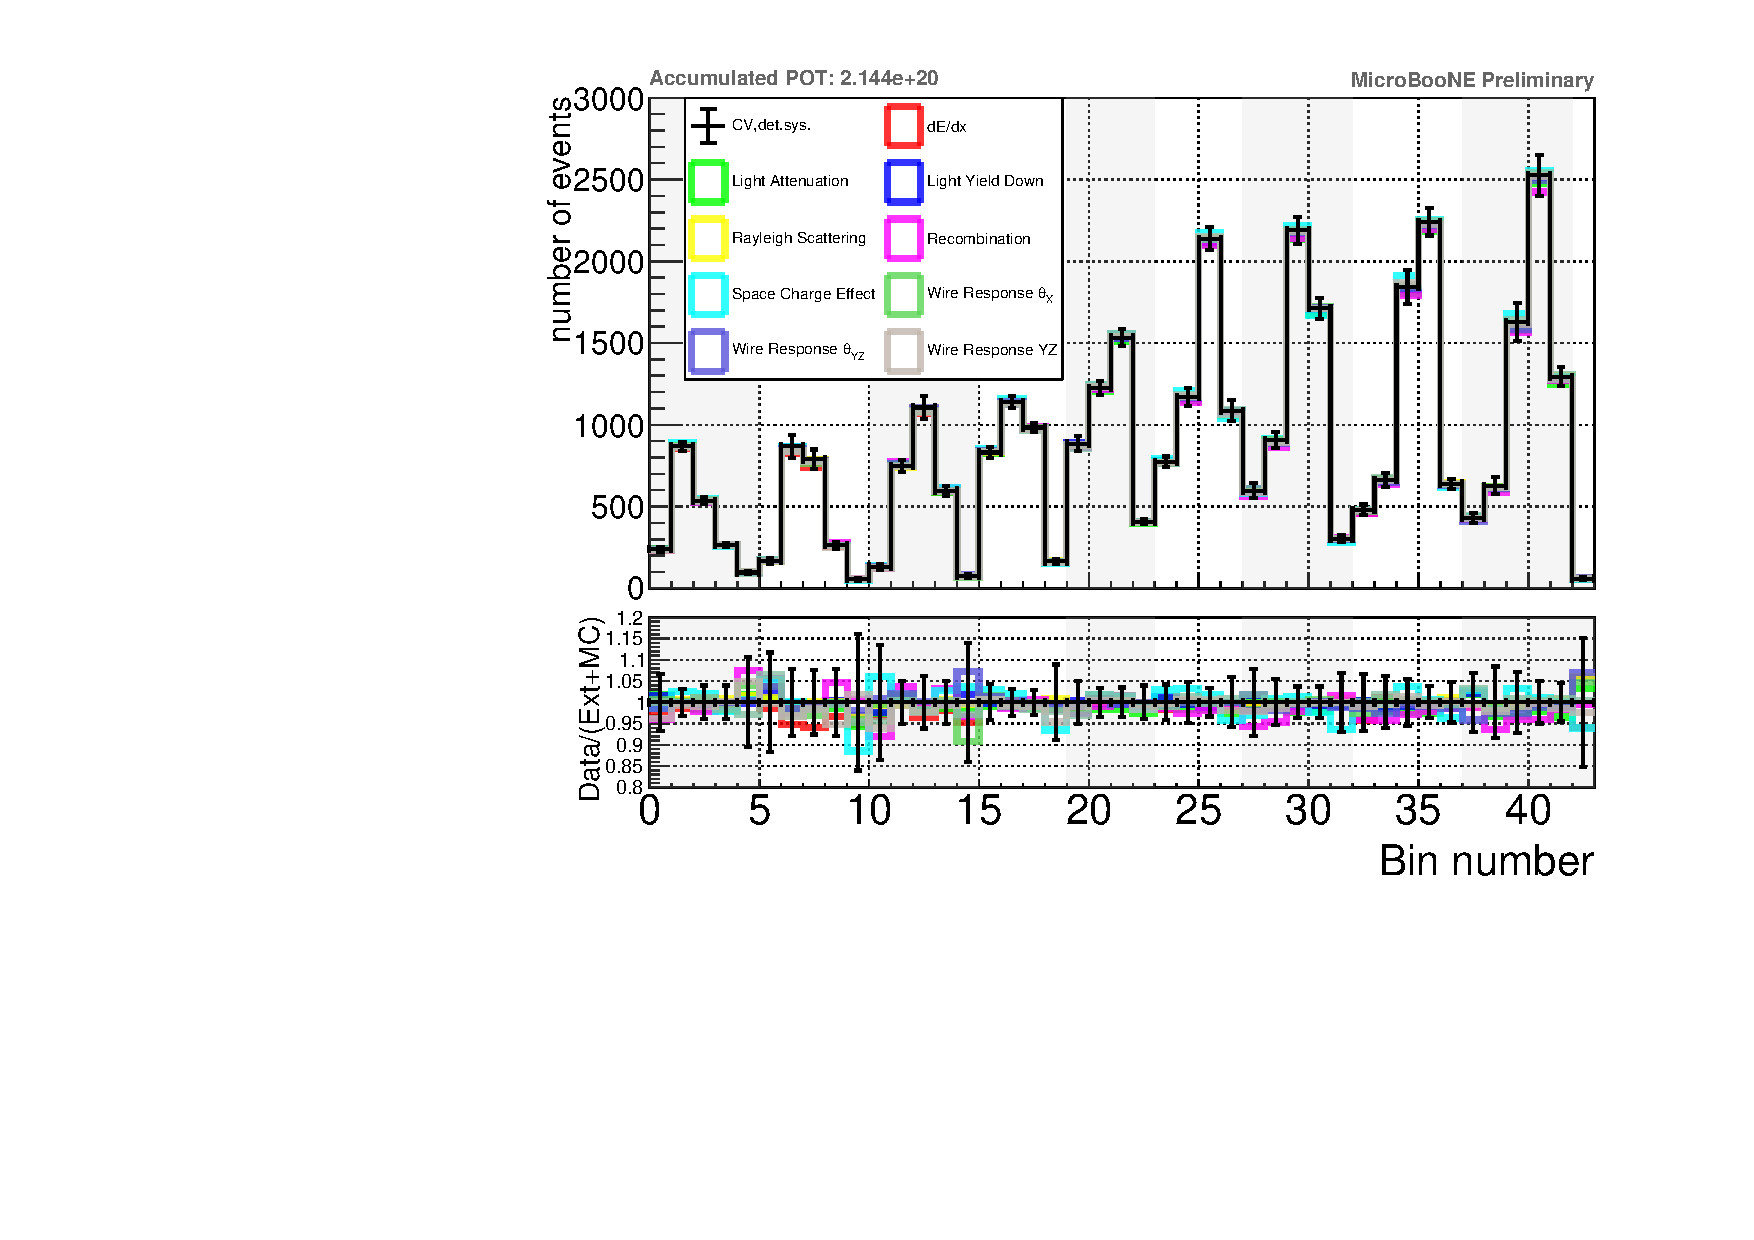
\includegraphics[width=0.49\textwidth]{images/NewCCInclusive/xsec/h_xsec_detsys.pdf}
            \label{fig:detsys}
        } \\
        \subfloat[GENIE all]
        {
            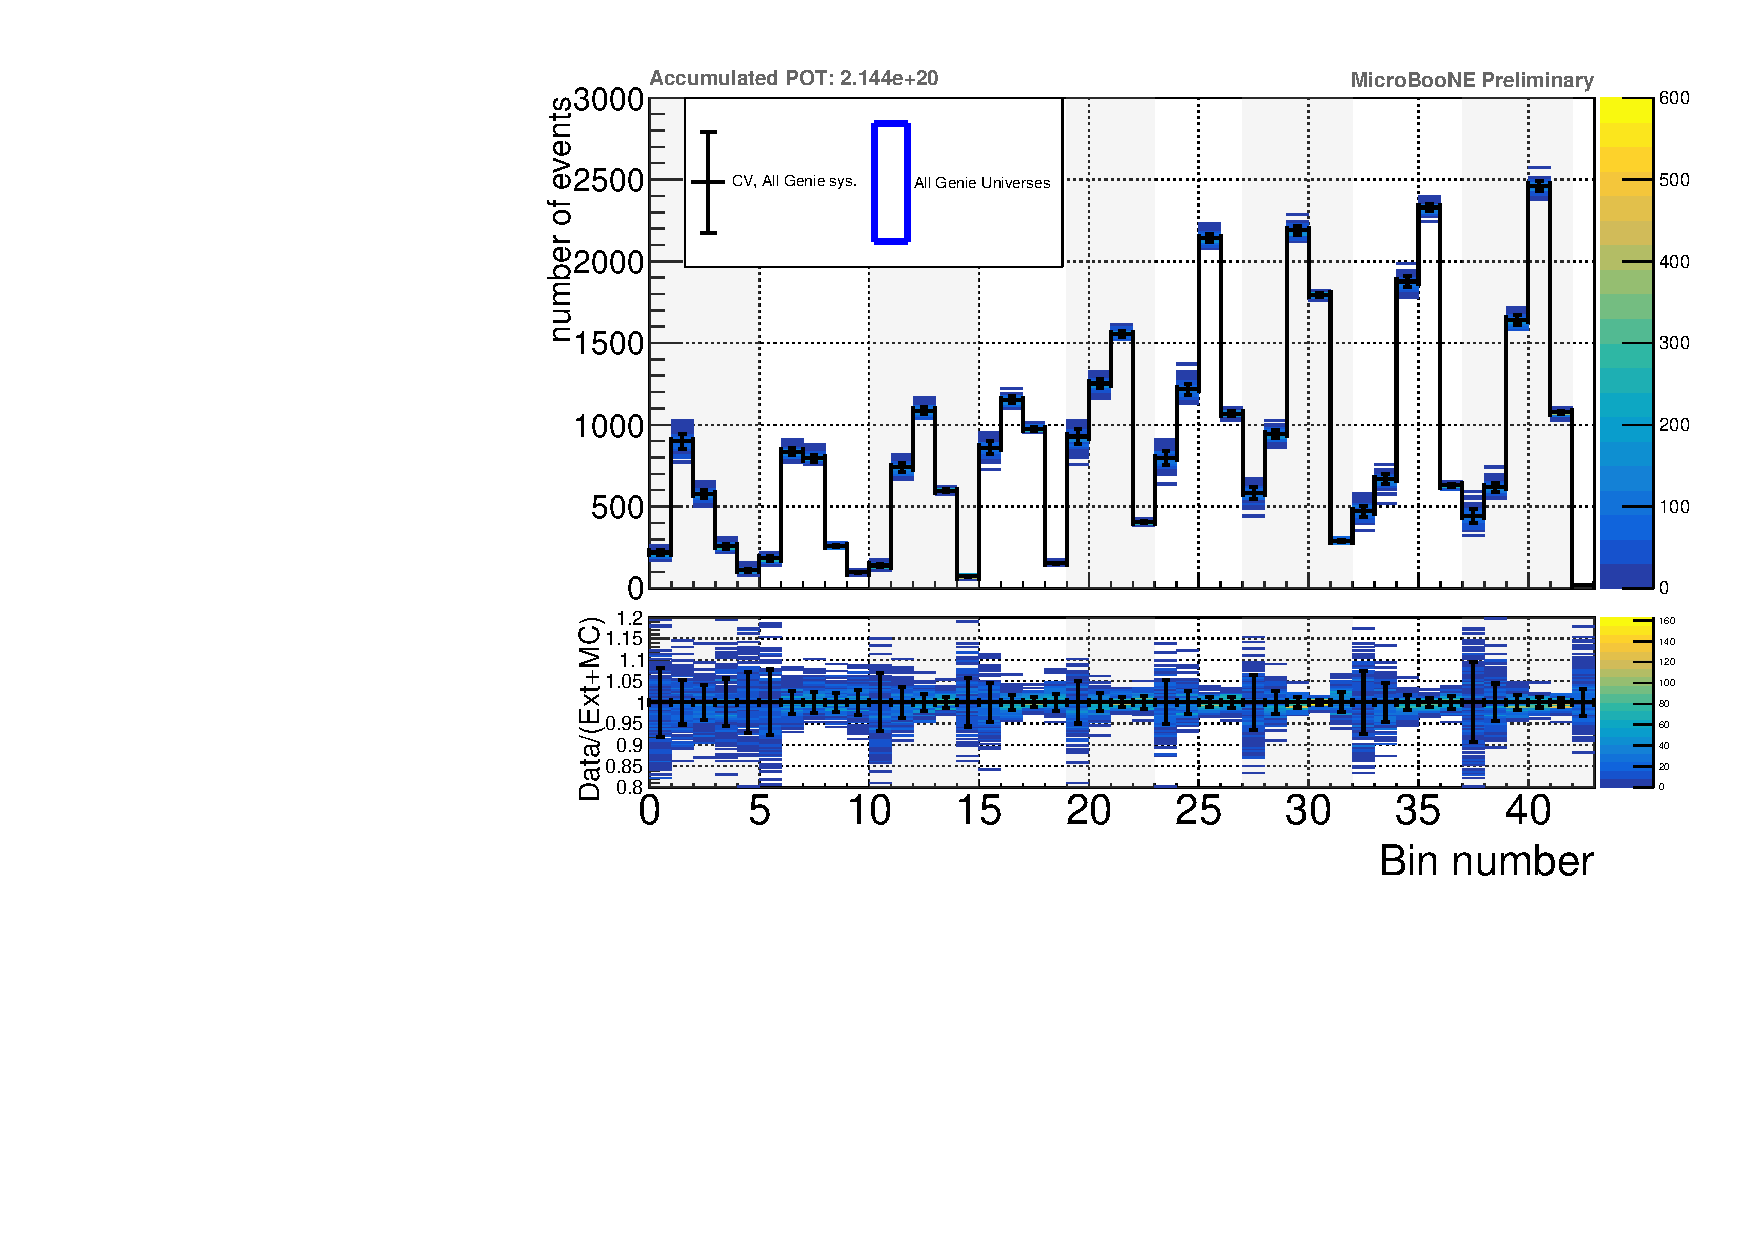
\includegraphics[width=0.49\textwidth]{images/NewCCInclusive/xsec/h_xsec_genie_allsys.pdf}
            \label{fig:xsecsys_tunedG3_all}
        }
		\subfloat[GENIE MicroBooNE]
        {
            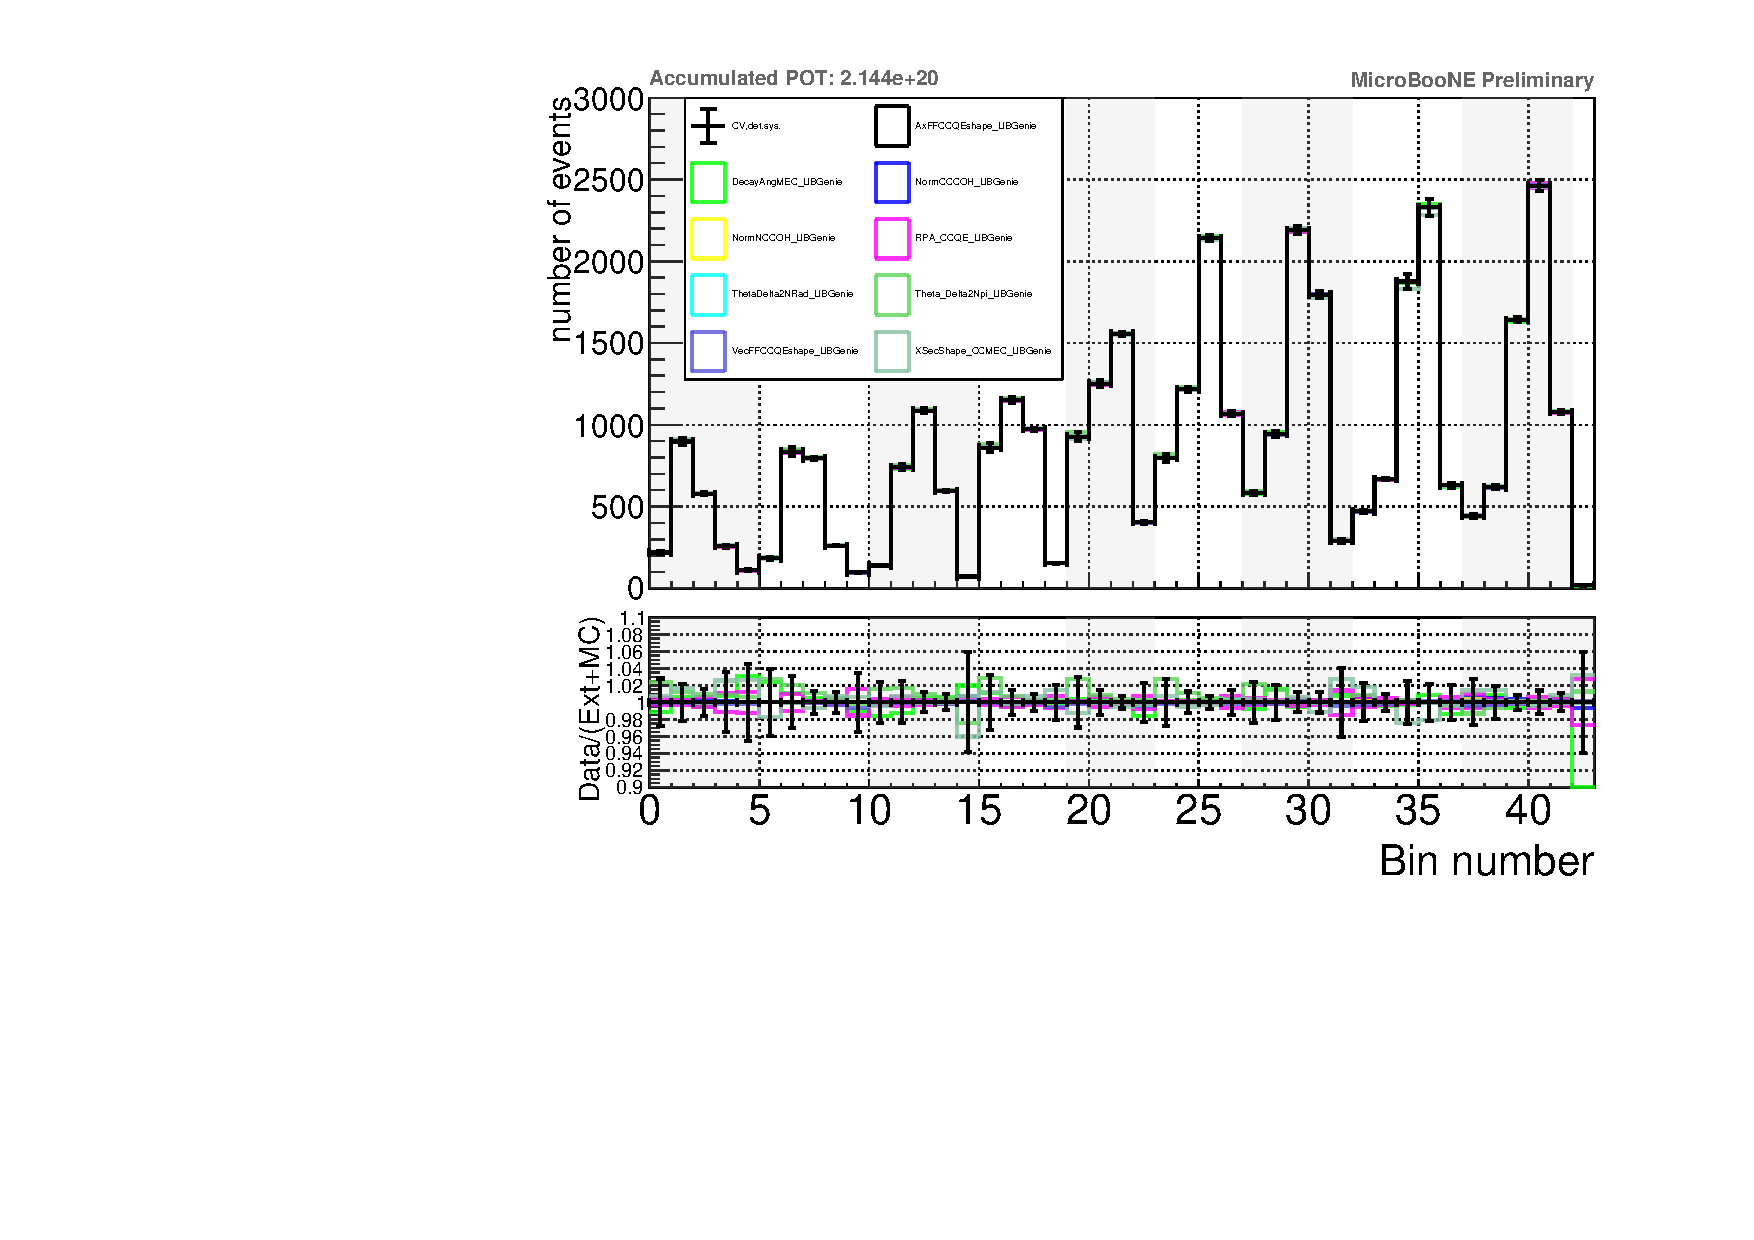
\includegraphics[width=0.49\textwidth]{images/NewCCInclusive/xsec/h_xsec_genie_uboone.pdf}
            \label{fig:xsecsys_tunedG3_uboone}
        } \\
        \subfloat[Dirt]
        {
            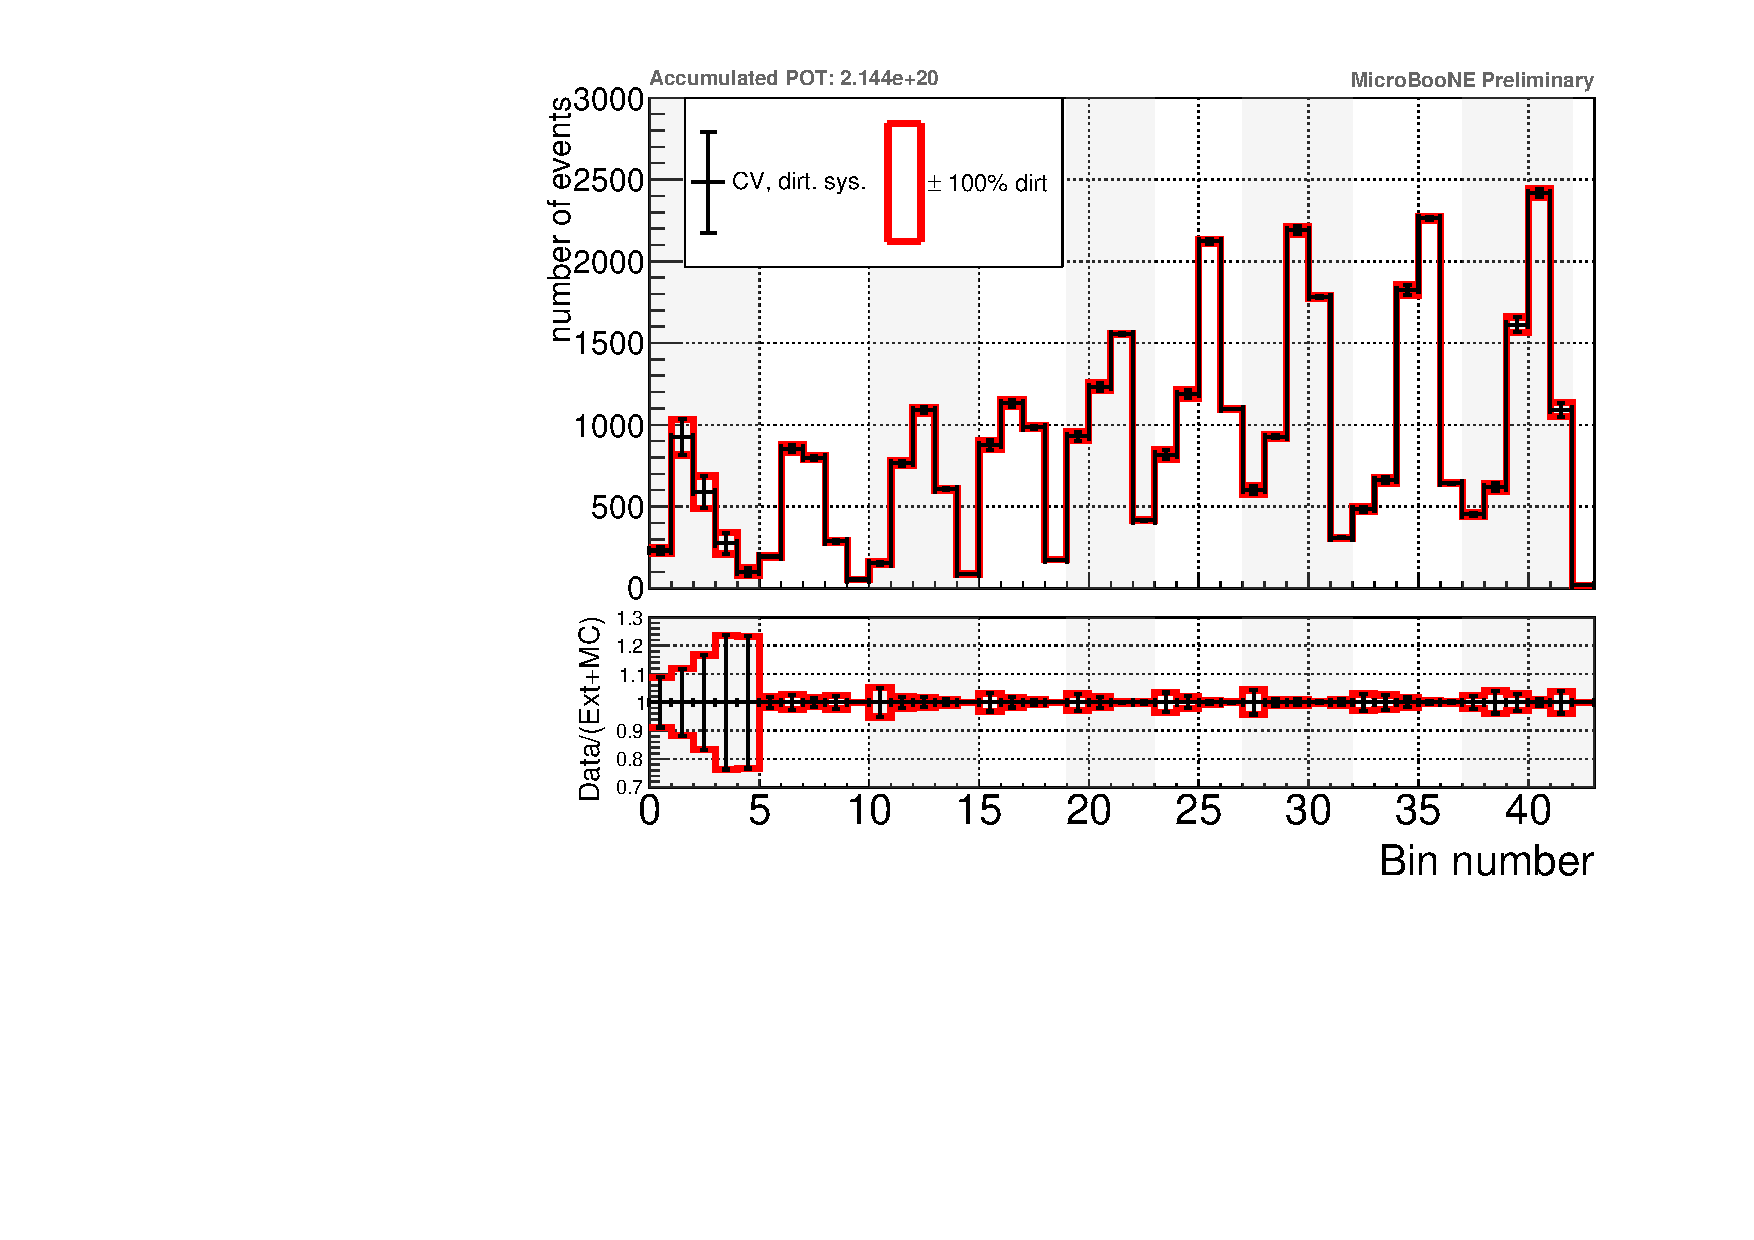
\includegraphics[width=0.49\textwidth]{images/NewCCInclusive/xsec/h_xsec_dirtsys.pdf}
            \label{fig:dirtsys}
        }
		\subfloat[CRT]
        {
            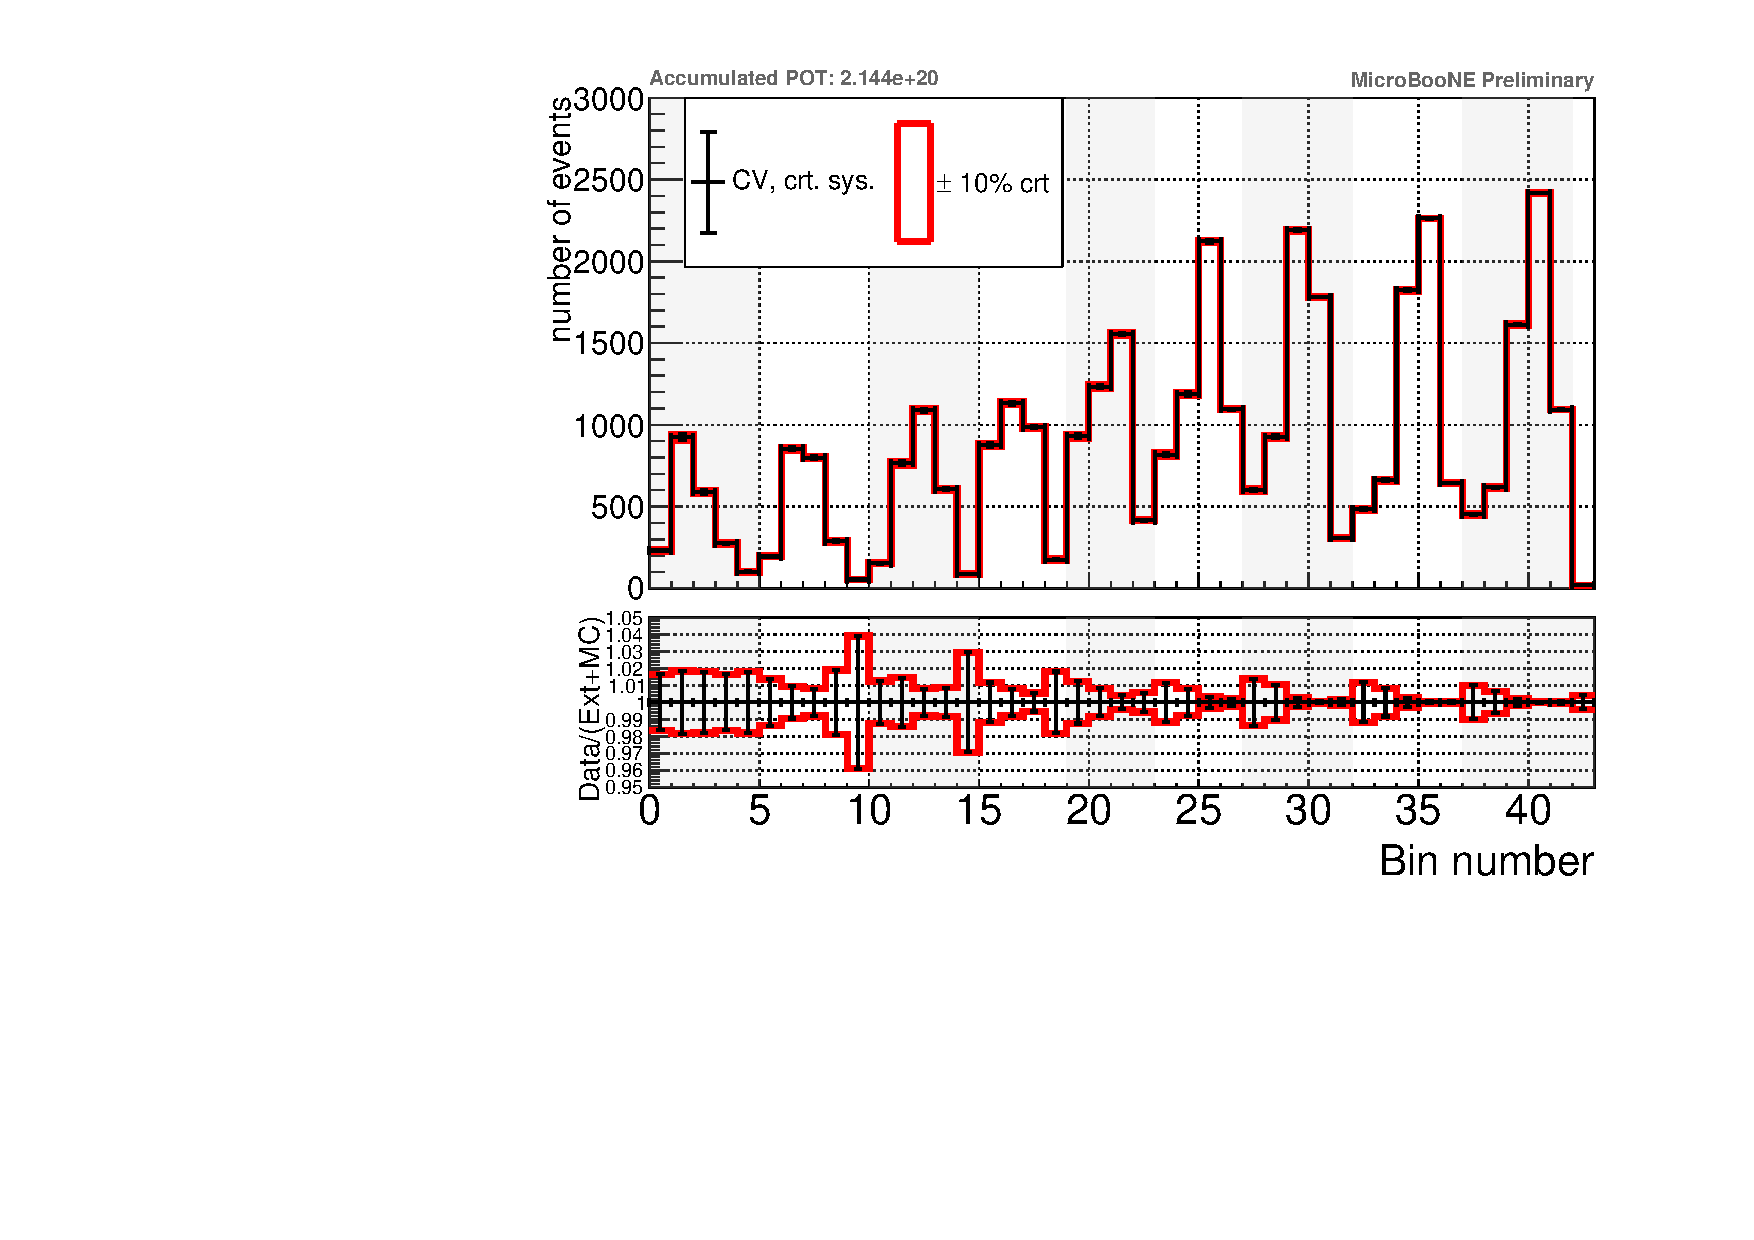
\includegraphics[width=0.49\textwidth]{images/NewCCInclusive/xsec/h_xsec_crtsys.pdf}
            \label{fig:CRT_uncertainty}
        }
        \caption[Multisim Results of Six Systematic Uncertainties]{Shown above are the results of various multisim examples, performed to determine the respective background systematics. All the graphs show depict the central value as a black data point, and the various universes, as coloured lines.} 
        \label{fig:SystematicUncertainties}
	\end{center}
\end{figure}


% \section{How to Forward Fold}
% 
% 
% \subsection{Background Prediction}\label{sec:NewBackgroundPrediction}
% The background prediction is simply put just the true distribution of all selected background events. It is shown in figure \ref{fig:bkg_tunedGENIEv3}, whereby the dashed blue, the brown and gray histograms are backgrounds from the three (\gls{mc}) data sets: the beam-off, dirt and overlay sample, respectively.
% \begin{figure}[htbp]
%   \centering
%   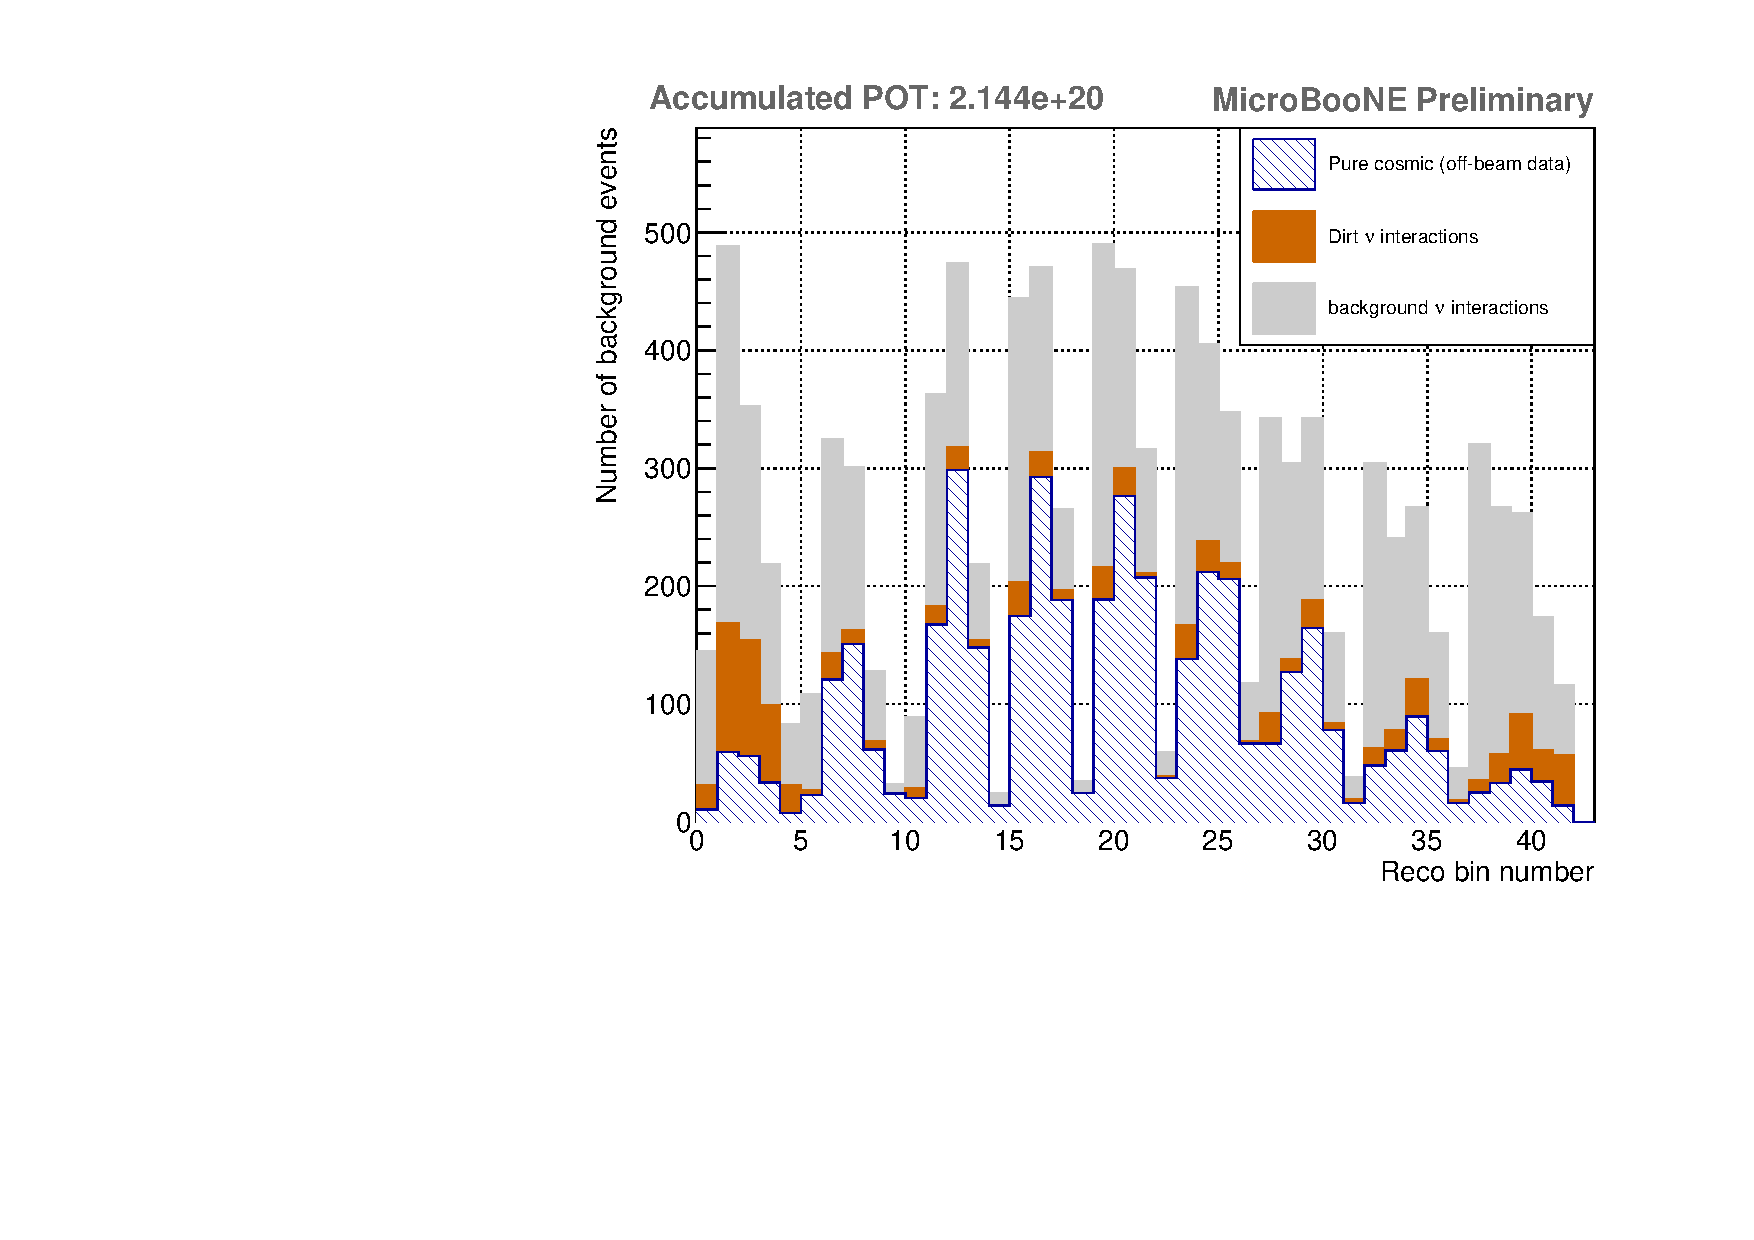
\includegraphics[width=0.7\textwidth]{images/NewCCInclusive/xsec/background_tunedGENIEv3.pdf}
%   \caption[Background Prediction]{The predicted background from beam-off (dashed blue), dirt (brown) and overlay (gray) samples in each reconstructed bin.}
%   \label{fig:bkg_tunedGENIEv3}
% \end{figure}
% The background prediction is needed for model comparison, where it is added to the model prediction with the proper \gls{pot} scaling. With the beam related backgrounds, we technically introduce a model dependency 
% However, as discussed in Sec.~\ref{subsec:numu_CC_sel}, more than half of the backgrounds are cosmic induced events, and each category of the neutrino backgrounds takes portion of much less than 5\% of the total selected events.
% It is not expected to improve the measurement significantly with substitutable background prediction.
% Furthermore, producing smearing matrices for the neutrino backgrounds is a non-trivial challenge, as the corresponding true particles for the reconstructed muons are ill defined.
% Therefore, we apply the same background prediction to all model comparison in this forward-folding measurement.
